%%
%% This is file `thesis.tex',
%% generated with the docstrip utility.
%%
%% The original source files were:
%%
%% nudtpaper.dtx  (with options: `thesis')
%% 
%% This is a generated file.
%% 
%% Copyright (C) 2015 by Liu Benyuan <liubenyuan@gmail.com>
%% 
%% This file may be distributed and/or modified under the
%% conditions of the LaTeX Project Public License, either version 1.3a
%% of this license or (at your option) any later version.
%% The latest version of this license is in:
%% 
%% http://www.latex-project.org/lppl.txt
%% 
%% and version 1.3a or later is part of all distributions of LaTeX
%% version 2004/10/01 or later.
%% 
%% To produce the documentation run the original source files ending with `.dtx'
%% through LaTeX.
%% 
%% Any Suggestions : LiuBenYuan <liubenyuan@gmail.com>
%% Thanks Xue Ruini <xueruini@gmail.com> for the thuthesis class!
%% Thanks sofoot for the original NUDT paper class!
%% 
%1. 规范硕士导言
% \documentclass[master,ttf]{nudtpaper}
%2. 规范博士导言
% \documentclass[doctor,twoside,ttf]{nudtpaper}
%3. 建议使用OTF字体获得较好的页面显示效果
%   OTF字体从网上获得,各个系统名称统一。
%   如果你下载的是最新的(1201)OTF英文字体,建议修改nudtpaper.cls,使用
%   Times New Roman PS Std
% \documentclass[doctor,twoside,otf]{nudtpaper}
%   另外,新版的论文模板提供了方正字体选项FZ,效果也不错哦
% \documentclass[doctor,twoside,fz]{nudtpaper}
%4. 如果想生成盲评,传递anon即可,仍需修改个人成果部分
% \documentclass[master,otf,anon]{nudtpaper}
%
\documentclass[master,otf]{nudtpaper}
\usepackage{mynudt}

\classification{TP957}
\serialno{0123456}
\confidentiality{公开}
\UDC{}
\title{基于多传感器的无人机自主着舰制导与控制技术研究}
\displaytitle{基于多传感器的无人机自主着舰制导与控制技术研究}
\author{孔维玮}
\zhdate{二〇一六年十二月}
\entitle{}
\enauthor{KONG Weiwei}
\endate{\entoday}
\subject{控制科学与工程}
\ensubject{Control Science and Engineering}
\researchfield{模式识别与智能系统}
\supervisor{沈林成\quad{}教授}
\cosupervisor{\quad{}} % 没有就空\quad{}着
\ensupervisor{Prof. SHEN Lincheng}
\encosupervisor{}
\papertype{工学}
\enpapertype{Engineering}
% 加入makenomenclature命令可用nomencl制作符号列表。

\begin{document}
	\graphicspath{{figures/}}
	% 制作封面,生成目录,插入摘要,插入符号列表 \\
	% 默认符号列表使用denotation.tex,如果要使用nomencl \\
	% 需要注释掉denotation,并取消下面两个命令的注释。 \\
	% cleardoublepage% \\
	% printnomenclature% \\
	\maketitle
	\frontmatter
	\tableofcontents
	\listoftables
	\listoffigures
	
	\midmatter
	%\begin{cabstract}
近年来,随着无人作战系统(Unmanned Combat System,UCS)在伊拉克、阿富汗等几场局部战争的广泛使用,展现了无人作战系统的巨大军事价值。作为无人作战系统中的重要组成,无人机所承担的侦察、监视、通信中继、战场评估、攻击引导等任务也日益增多。为扩大无人机的工作半径,提升作战效能,无人机在舰船上回收的需求更加迫切。虽然无人机在地面起飞、降落或回收已经成为常态,但上述过程中的引导方式主要依赖卫星定位导航系统(Global Navigation Satellite System,GNSS)。在未来“反介入/区域拒止(A2/AD)”的战场环境下,仅仅依赖卫星导航系统无法满足无人机在舰船的降落需求。本文主要针对上述研究背景展开工作,主要完成工作和创新点如下:

(1)提出了一种地基/舰基通用的多传感器无人机回收引导系统。该系统主要有两个独立引导单元组成,每个引导单元配备一个二自由度转台和可见光相机、红外相机等传感器。两个独立引导单元的排布可以根据目标无人机的大小和检测距离进行优化配置。本文针对该系统独立分布在跑道两侧的特点,通过对目标位置解算理论推导、误差分析和实验验证,证明了在无人机降落过程中,使用上述两种引导系统的可行性。

(2)设计并实现无人机降落过程中实时目标跟踪和位置解算算法。针对引导无人机降落过程中,无人机目标尺度快速变化和姿态未知的问题,通过改进基于形态学滤波的图像预处理方法,TLD目标跟踪框架和基于主动轮廓的目标位置修正方法,结合转台运动位置和无人机运动的估计,能够准确解算出无人机在降落过程中相对于舰船的位置信息,满足无人机引导和控制系统的需要。

(3)设计并实现基于非线性模型预测控制(NMPC)和总能量控制(TESC)的无人机着舰控制系统。由于无人机机载设备运算能力的约束,本文设计了内环控制器和外环控制器来实现无人机的自主降落。其中内环控制器主要由PI和PID控制器组成,主要完成对无人机姿态的控制;外环控制器主要由非线性模型预测控制器(NMPC)和总能量控制器(TESC)组成,针对基于Dubins Path生成的降落曲线进行跟踪。

(4)设计并实现无人机舰载着舰系统仿真环境并进行户外实验验证。本文基于机器人操作系统(Robot Operation System,ROS)和Gazebo仿真环境构建了无人机舰载着陆软件在回路仿真系统(SITL)和硬件在回路仿真系统(HIL)。该仿真环境能够满足上述算法的验证需求。通过二自由度转台与多传感器的组合配置,实现在地面机场和水面环境对小型和中型固定翼无人机的引导和自主降落。

上述理论和算法成果分别发表在2012年和2013年的IEEE/RSJ智能机器人与系统国际会议(IROS)会议,得到了领域内同行的认可。基于上述算法的实际飞行测试分别在江西吉安机场和湖南长沙湘江水域进行,验证了基于多传感器的地基引导系统和舰基引导系统的可行性和可靠性。

\end{cabstract}
\ckeywords{无人机;自主着舰;多传感器引导与控制;}

\begin{eabstract}
 In recent years, with the unmanned combat system(UCS) in Iraq, Afghanistan and several other local wars of widespread use, unmanned combat system is showing the great military value. As an important component of unmanned combat system, unmanned aerial vehicles(UAVs) are increasingly assigned with reconnaissance, surveillance, communication relay, battlefield evaluation and attack guidance. In order to expand the operating radius of UAV, improve combat effectiveness, the demand of autonomous landing on a destroyer or carrier is continuing to grow. Although UAVs take off and landing on the standard airport is quite common, navigation in the above maneuvers relies mainly on the Global Navigation Satellite System (GNSS). In the future A2 / AD battlefield environment, the satellite navigation system alone can not meet the UAVs' landing demand. This paper aims at the above research background, the main work and innovation are as follows:
 
(1) A ground / ship-based multi-sensor unmanned aerial vehicle (UAV) recovery and guidance system is proposed. The system consists of two independent guidance units, each with a two degrees of freedom PTU(Pan/Tilt Unit) and visible light camera, infrared camera or other sensors. The configuration of the two independent guidance units can be optimally setup according to the size of the UAV and the proposed detection distance. In this thesis, the feasibility of using the above two guidance systems in the process of UAV landing is proved by the theory of target position solution, error analysis and experimental verification, which is based on the characteristics of the system distributed on both sides of the runway independently.

(2) Design and implement the real-time target tracking and location algorithm in UAV landing process. Aiming at the problem of traking the UAV, size rapidly changing from tiny to large scale, the method of image preprocessing based on morphological filtering, TLD target tracking framework and target position updating based on active contour are improved. During the landing process, the Motion position and unmanned aerial vehicle motion estimation, can accurately calculate the position of UAV relative to the ship's position 

(3) Design and implementation of the non-linear model predictive control (NMPC) and total energy control (TESC) of the UAV landing control system. Due to the computation constraints of UAV on-board equipment, the inner-loop controller and the outer-loop controller are designed to realize the autonomous landing. The inner loop controller is mainly composed of PI controller and PID controller. The outer loop controller mainly consists of nonlinear model predictive controller (NMPC) and total energy controller (TESC) in order to tracking the landing curve which generated by Dubins Path algorithms.

(4) Design and implement the simulation system and experimental verification system for UAV shipboard landing problem. Based on the Robot Operation System (ROS) and Gazebo simulation environment, a software in the loop simulation system (SITL) and hardware in the loop simulation system (HIL) is constructed. The simulation environment can meet the verification requirements of the above algorithms. By selecting PTUs and reltaed sensors, autonomous guidance and landing of the UAV can be achieved at ground and airfields.

The above theoretical and algorithmic results were published in the 2012 IEEE / RSJ Intelligent Robot and Systems International Conference (IROS) meeting in 2012 and were recognized by peers in the field. The actual flight tests based on the above algorithms were carried out in Ji'an Airport of Jiangxi Province and Xiangjiang River of Changsha, Hunan Province, respectively. The feasibility and reliability of the foundation guidance system and ship-based guidance system based on multi-sensor were verified.
 
 
\end{eabstract}
\ekeywords{UAV; Autonomous Landing; Multi-sensor Guidance and Control}

  摘要
	%\chapter*{符号使用说明}
% 可以根据需要在chapter后加星星/去掉星星

\begin{denotation}

\item[HPC] 高性能计算 (High Performance Computing)
\item[cluster] 集群
\item[Itanium] 安腾
\item[SMP] 对称多处理
\item[API] 应用程序编程接口
\item[PI]	聚酰亚胺
\item[MPI]	聚酰亚胺模型化合物,N-苯基邻苯酰亚胺
\item[PBI]	聚苯并咪唑
\item[MPBI]	聚苯并咪唑模型化合物,N-苯基苯并咪唑
\item[PY]	聚吡咙
\item[PMDA-BDA]	均苯四酸二酐与联苯四胺合成的聚吡咙薄膜
\item[$\Delta G$]  	活化自由能~(Activation Free Energy)
\item [$\chi$] 传输系数~(Transmission Coefficient)
\item[$E$] 能量
\item[$m$] 质量
\item[$c$] 光速
\item[$P$] 概率
\item[$T$] 时间
\item[$v$] 速度

\end{denotation}
  贡献
	
	%书写正文,可以根据需要增添章节; 正文还包括致谢,参考文献与成果
	\mainmatter
	%\chapter{绪论}


\section{研究背景和意义}
无人机(UAV, Unmanned Aerial Vehicles)在最近十年中已经成为科技领域最吸引眼球的“关键词”。由于无人机自身具有成本低、机动性好、隐蔽能力强等特点,许多国家开展了基于无人机平台的各类研究。回顾历史,自1918年3月6日第一架现代无人机的出现距今已经近百年的历史,但在现实生活中,由于其安全性、可靠性等原因,无人机离我们的生活仍存在着一定的距离。特别是无人机在户外应用过程中,引导信息主要通过将卫星定位导航系统(Global Navigation Satellite System,GNSS)与惯性导航信息相互融合得到。因此,在GNSS信号较弱或者发生中断的情况下,每年在世界各地均发生多起无人机坠毁事件,带来了巨大的人员和经济损失的同时,也限制了无人机的快速应用和发展。

在这些事故中,无人机操作员的失误导致的事故率高达60\%\cite{arrabito2010human}。在2004年的一份报告中指出\cite{williams2004summary},无人机的起飞和降落阶段过程中,人为因素的影响接近50\%。因此,研究精确可靠、自动化程度较高的着陆系统对无人机装备的战斗力生成至关重要,同时也是无人机通用技术发展的关键环节。下面针对自主起降技术的民用需求和军用需求展开说明。

\subsection{无人机引导回收的民用需求}
近年来,随着我国经济的快速发展和人民生活收入水平的提高,越来越多的人选用民航作为出行手段,因此带来航班密度的显著增加。与此同时,气候原因与空气污染的综合作用导致航班晚点情况愈发严重。为研究气候原因导致飞机无法正常降落的情况,有文章\cite{BigDataLanding}通过分析2012年到2014年春运期间的民航数据(CADA, Civil Aviation Data Analysis)得出:影响航班准点率的雾、雪、霾天气所占比例为28.09\%;在千万级级别机场中,霾影响最严重的是郑州机场,占比例为29.21\%,其次是西安机场,所占比例为26.05\%;而在受雾影响的机场中,长沙机场占39.74\%,武汉机场占32.41\%,西安机场占32.07 \%。由此可见,在航班密度最大的春运期间,航班受天气影响导致延误的比例很大。

与人们直观的认知不同,航班是否能够安全降落,除飞机自身性能外,主要取决于目标机场的可见度情况,根据国际民航通用准则,飞机降落标准由低至高主要分为三类:CAT I类,其决断高度(DH, Decision Height)为$60\ m$、跑道视距(RVR, Runway Visual Range)为$550\ m$;CAT II类,DH为$30\ m$、RVR为$300\ m$;CAT III类,其DH和RVR均为$0\ m$要求,即为真正意义上的盲降。目前,国内除北京、浦东、成都、西安为II类机场外,多数机场为I类,而国内大多数航空公司只能执行I类标准,如果天气条件低于I类,航班就无法降落,只能选择备降或返航,影响航班正点率。因此,如果能够通过辅助设备,提高和拓展飞行员的可见度,则可以显著降低因为能见度原因导致的航班延误,从而提高民航的准点率。

在民用无人机领域,大量的无人机的回收依赖GNSS导航信息,加之没有配套的地面或舰载辅助引导设备,无人机的广泛应用受到了较大限制。

\subsection{无人机引导回收的军事需求}
在军事领域,飞行器的自主起降需求则更为迫切。在有人机方面,随着2012年11月23日,歼-15战斗机首次在航母上成功实施阻拦着舰和滑跃起飞(如图\ref{fig:22_J15Landing_Big}所示),航母舰载机的引导降落问题再次引起世人关注。一般而言,为了保证舰载机正确返航和着舰,现代航母均配备有战术空中导航系统、空中交通管制系统和着舰引导系统。完整的着舰过程实质上是一场接力导航:当距离航母300公里时,归航舰载机由战术空中导航系统指挥引导;距离100公里时,由空管雷达接手;距离30公里时,再次由战术空中导航系统引导;距离10公里时,自动着舰系统开始引导;距离3公里时,进入舰上光学助降系统工作区域,最后据此着舰。

\begin{figure}[htb]
	\centering%
	\subfloat[X-47B着舰钩索的瞬间]{%
		\label{fig:01_X47B_Landing}
		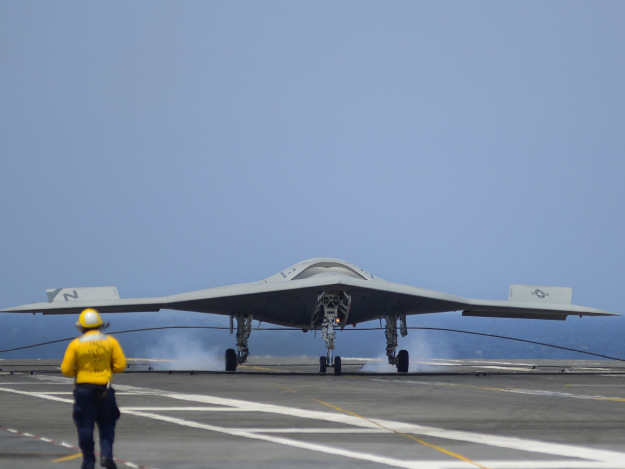
\includegraphics[height=5cm]{Figs/01_X47B_Landing.jpg}}\hspace{0.7em}%
	\subfloat[歼15着舰钩索的瞬间]{%
		\label{fig:22_J15Landing_Big}
		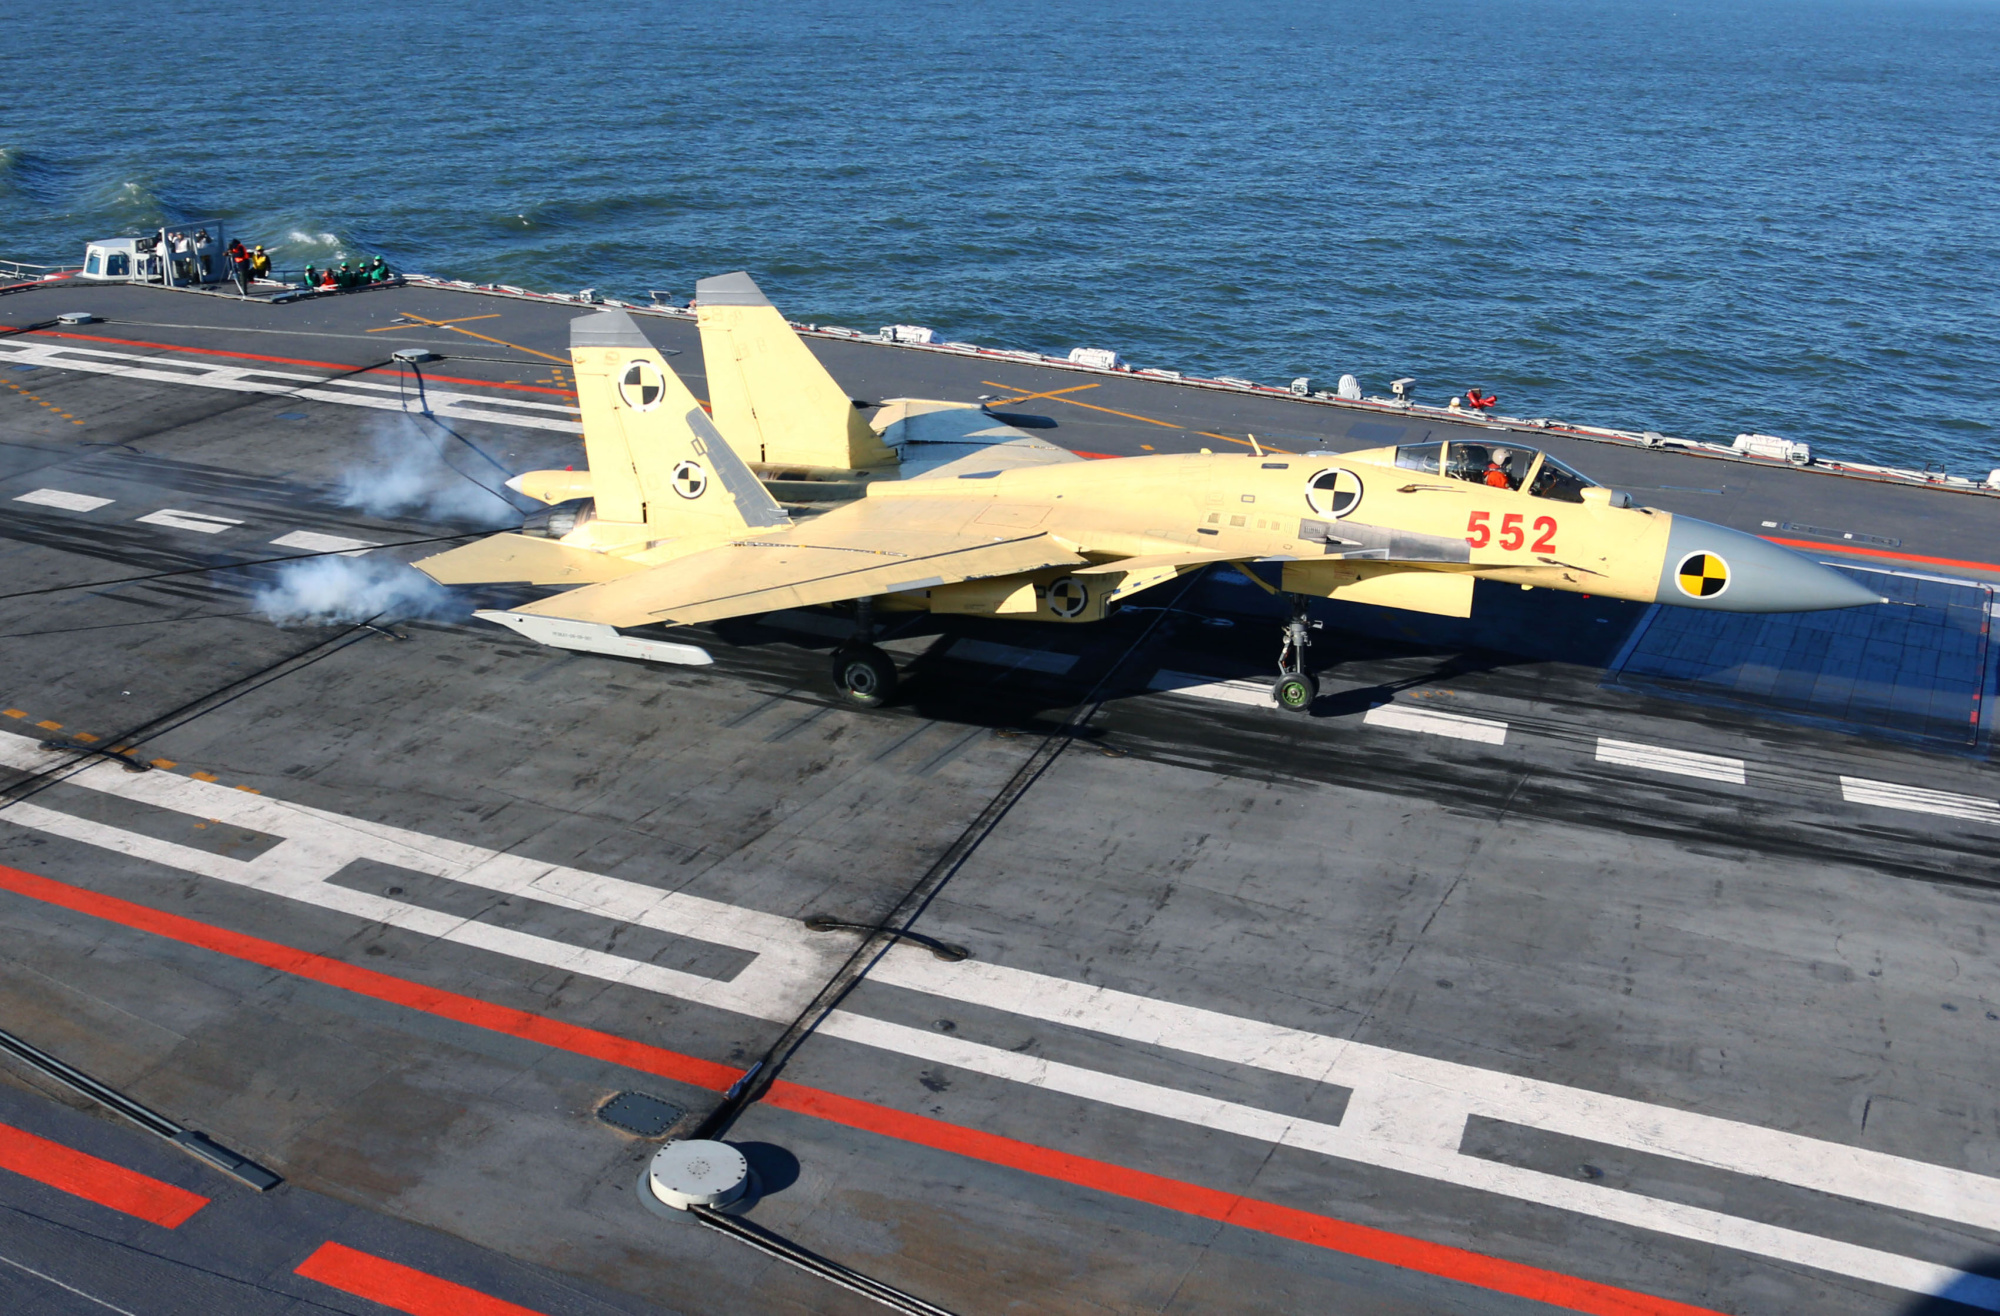
\includegraphics[height=5cm]{Figs/22_J15Landing_Big.jpg}}
	\caption{中美海军飞行器着舰瞬间}
	\label{fig:01_Landing}
\end{figure}

在舰载机降落过程中,飞行员除利用光学助降系统提供的信息进行修正外,航母舰舰载机着陆通常还依赖于人工辅助降落信息。在美航母上,通常由6人组成的着舰信号官(Landing Signal Officer,LSO)位于航母着舰区后部左舷,依靠视频监视系统所拍摄的实时图像及相应参数,通过无线电及灯光等多种手段对舰载机飞行员发出相应着舰指令(如图\ref{fig:20_LSO_USA}所示)。这6人分工和人员配置:(1)担当舰载机着舰引导操作的LSO;(2)利用飞行员助降视频(HUD)显控台引导飞机进场着舰顺序的助理LSO;(3)记录着舰成绩/等级的见习LSO;(4)担任舰内联络的下士联络员;(5)舰载机着舰前尾钩、起落架、襟翼状态的观察员;(6)负责监察着舰引导小组工作的负责人。而在公开的资料中,我国的有人机着舰也采用了类似LSO的人工辅助引导手段,其工作状态如图\ref{fig:21_LSO_China}所示。

\begin{figure}[htb]
	\centering%
	\subfloat[我国“辽宁号”航母上的LSO]{%
		\label{fig:21_LSO_China}
		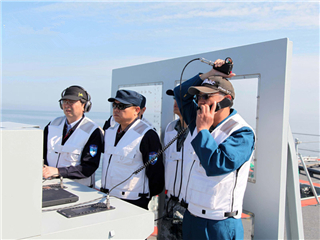
\includegraphics[height=4cm]{Figs/21_LSO_China.jpg}}\hspace{4em}%
	\subfloat[美军航母上的LSO]{%
		\label{fig:20_LSO_USA}
		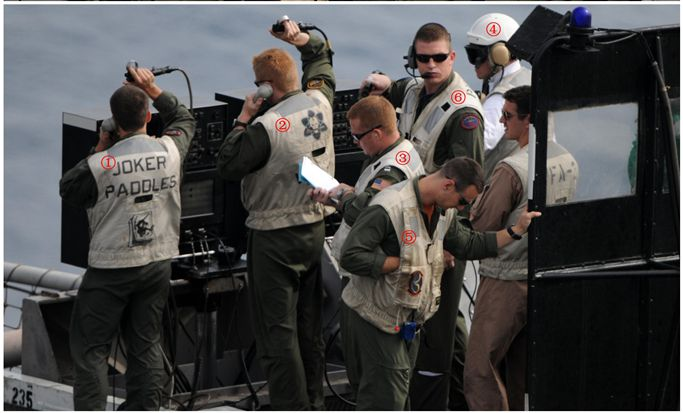
\includegraphics[height=4cm]{Figs/20_LSO_USA.jpg}}
	\caption{中美两国海军LSO工作图}
	\label{fig:21_LSO}
\end{figure}

无人机方面,在降落阶段无人机往往变成了“有人机”,一般会有多个人员进行操控和监视,以免出现差错。所以,本来希望减少人员工作负担的无人机,在降落阶段却往往成为让人担心的“微型炸弹”。为解决无人机的自主起降问题,早在2007年,美国诺斯鲁普·格鲁曼公司开始基于X-47B无人机和美国海军“无人作战航空系统-验证机”(UCAS-D)项目,开发和验证一种自主起飞/拦阻着舰型无人作战飞机。项目合同规定,诺格公司需要研制两架X-47B验证机,完成在航母上自主起降能力的验证,并在完成与航母一体化验证试验后,验证空中自主加油能力。如图\ref{fig:14_LandingAreaX47B2}所示,美国为开展相关研究,在Patuxent River试验基地展开岸基测试,并绘制了模拟甲板起降范围的模拟跑道(如图\ref{fig:10_LandingAreaX47B1}黄色箭头所示),这些细节体现了美国军方对这项技术的重视程度。
\begin{figure}[htb]
	\centering%
	\subfloat[位于海岸边的美军Patuxent River试验基地卫星图片]{%
		\label{fig:14_LandingAreaX47B2}
		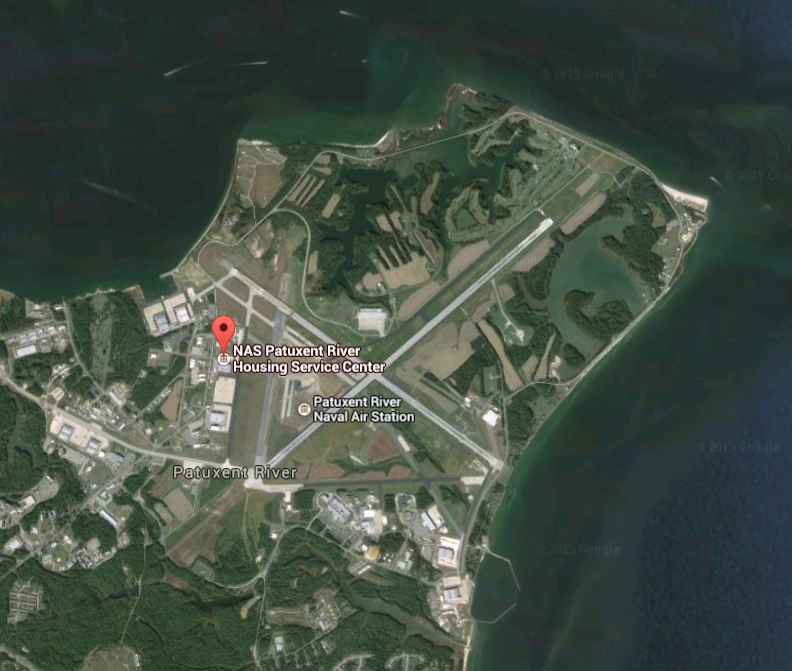
\includegraphics[height=6cm]{Figs/14_LandingAreaX47B2.jpg}}\hspace{0.7em}%
	\subfloat[黄色箭头所指为模拟航母甲板区域的专用跑道]{%
		\label{fig:10_LandingAreaX47B1}
		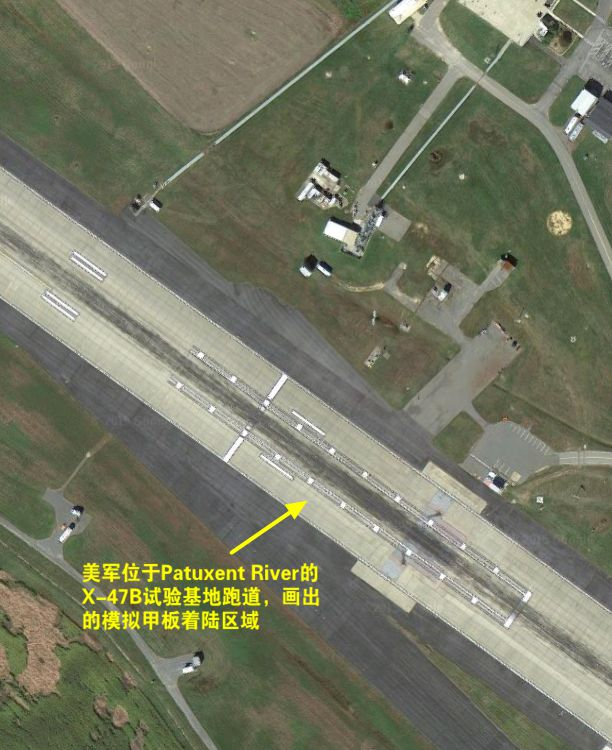
\includegraphics[height=6cm]{Figs/10_LandingAreaX47B1_1.jpg}}
	\caption{美军Patuxent River试验基地}
	\label{fig:14_LandingAreaX47B}
\end{figure}

在沉寂消息多年后,2013年7月,X-47B完成举世瞩目的首次航母自主降落,如图\ref{fig:01_X47B_Landing}所示)。根据公开资料显示\cite{X_47B},X-47B总共完成37次接触甲板测试(Deck Touchdown Test)和30次复飞(Touch-and-go)测试。在2014年3月,由于X-47B及其配套系统完成了人类历史上首次无人飞行器在航空母舰的全自主测试,“X-47B技术团队”获得美国航空协会最重要的“罗伯特·科利尔奖(Robert J. Collier Trophy)”\cite{X_47B_Award}。值得关注的是,该奖项曾经颁奖给诸多美国军用项目,如“全球鹰”无人机系统、“大黄蜂”战机系统、B2轰炸机系统等,由此可见X-47B及其配套系统在理论和工程上所具有的重要意义。此外,在各类报道中也特别提到:该系统精确的导航系统满足了飞行器降落在运动中的航母甲板上,具有里程碑意义\cite{X_47B_Report}。2014年8月,X47-B开展进一步测试,在完成与F/A-18F联合飞行验证后,在90秒内完成自主着舰、折叠机翼、撤出着舰区等一些列动作。其中,4次拦阻着陆,9次复飞再着陆。由于其优秀的控制性能,同月,美国海军计划利用X-47B开展空中自主加油的验证。根据公开资料判断,X-47B的降落除机载传感器外,舰载的JPALS或类似的雷达系统应当提供了辅助信息,如图\ref{fig:X47B_LandingOptical}所示。

\begin{figure}[htb]
	\centering%
	\subfloat[X-47B公布的视频中,跑道一侧的疑似毫米波雷达引导系统]{%
		\label{fig:09_X47BwithRadarGround}
		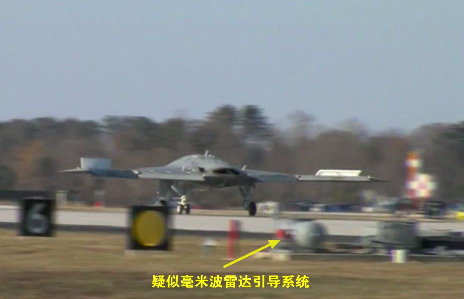
\includegraphics[height=5.2cm]{Figs/09_X47BwithRadarGround.pdf}}\hspace{1em}%
	\subfloat[X-47B公布的视频中,位于舰岛的疑似毫米波雷达引导系统]{%
		\label{fig:02_X47B_LanidngwithRadar1}
		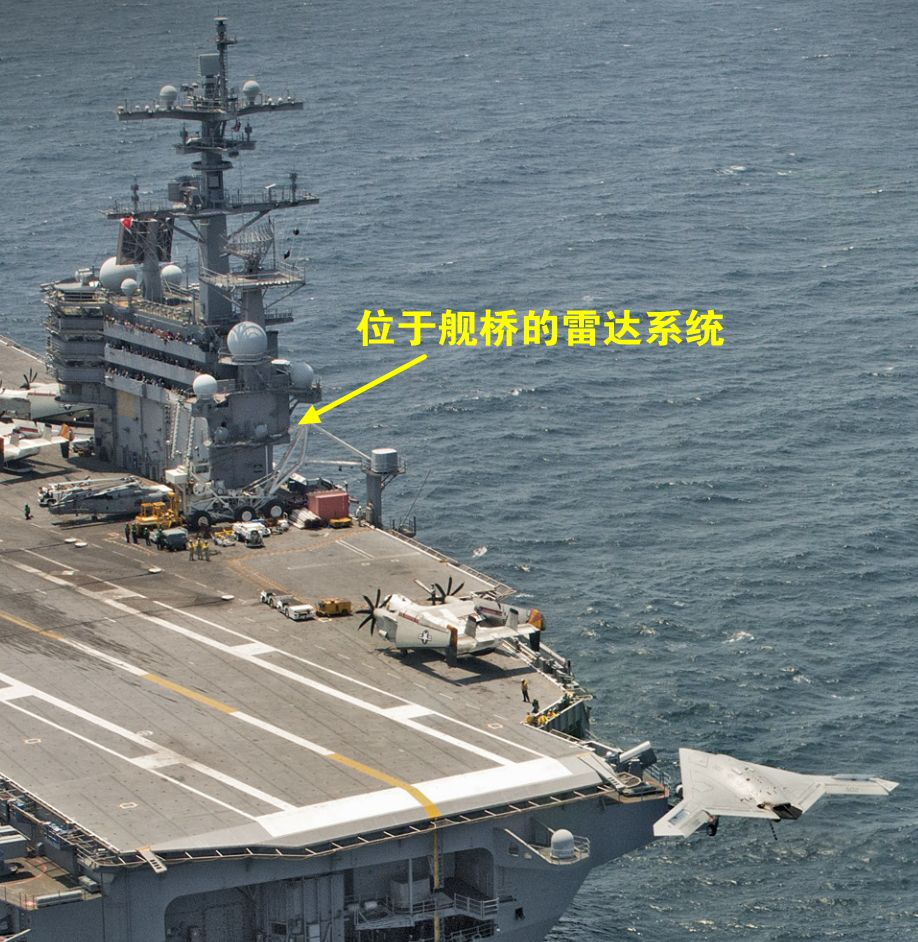
\includegraphics[height=5.2cm]{Figs/02_X47B_LanidngwithRadar1.jpg}}
	\caption{X-47B疑似使用的引导系统}
	\label{fig:X47B_LandingOptical}
\end{figure}



除X-47B这一机型之外,在2014年出版的《2030年的武器装备》\cite{2030equipment}一书中提到,作为美军太空机动飞行器的验证机型X-37B轨道飞行器(OTV, Orbital Test Vehicle),其在返回过程中,运用航空器的导航与指导技术,采用惯性导航和GPS的组合式导航方式,在接近跑道前,以20°的下滑角,350 km/h的速度进场,其降落过程和姿态与X-47B相似(如图\ref{fig:31_X37B_Landing}所示)。根据公开资料显示,X-37B的自主再入和着陆系统采用了惯性导航和GPS的组合式导航。截至到2014年10月17日,X-37B已经完成三次飞行试验,其再入与着陆技术得到波音公司和美国军方的认可。此外,根据2015年2月23日的公开报道,X-37B轨道测试飞行器团队(X-37B Orbital Test Vehicle Team)荣获2015年美国AIAA颁发的年度最高奖项——杰出贡献奖(Award for Excellent)\cite{X_37B}。在颁奖的公告中特别提到,自主降落技术是X-37B的关键技术之一。

\begin{figure}[htb]
	\centering%
	\subfloat[X-37B降落沿跑道方向正视图]{%
		\label{fig:31_X37B_Landing1}
		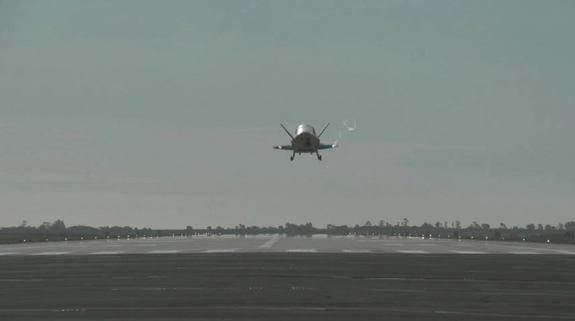
\includegraphics[height=4cm]{Figs/31_X37B_Landing1.jpg}}\hspace{0.7em}%
	\subfloat[X-37B降落侧视图]{%
		\label{fig:32_X37B_Landing2}
		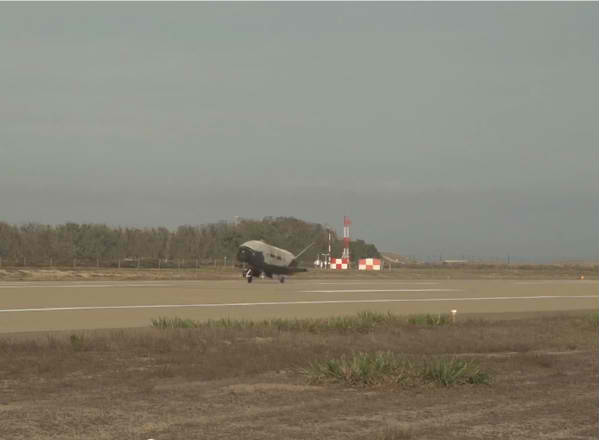
\includegraphics[height=4cm]{Figs/32_X37B_Landing2.jpg}}
	\caption{X-37B完成自主降落}
	\label{fig:31_X37B_Landing}
\end{figure}

综上所述,无人机自主起降技术,特别是舰载无人机自主起降技术是无人机广泛使用的基础和关键。能够在舰载环境,完成无人机的自主回收工作,具有很大的现实意义。


\section{军事和工业领域的引导降落系统}
\subsection{普通飞行器引导降落系统}
\subsubsection{仪表着陆系统}
在航空业发展初期,仪表着陆系统(ILS, Instrument Landing System)作为飞行器的主要着陆手段。该系统于1919年通过美国国家标准局的试验,并在二次大战期间得到广泛应用。1949年,国际民航组织规定仪表着陆系统作为着陆系统的国际标准。该系统主要由地面站和机载设备组成,主要通过机载接收机解算由地面航向信标和下滑信标独立产生的水平和交叉方向波束(波束频率不同),得到飞机的位置信息,即方位角、仰角和距离。该系统的示意图如图\ref{fig:07_ILS}所示。同时,民航组织根据需要,对不同气象条件下的进场标注进行了明确规定。其中,CAT I级别的高度主要通过气压计进行判读,CAT II和CAT III主要通过雷达高度计(Radio Altimeter)进行判读,不同级别的决断高度是飞行员做出是否复飞的基本准则。该系统的优点是具备较好的引导能力,可以为飞行员提供有效方位信息。但在当前电磁频谱环境复杂的机场附近,往往难以得到理想的引导控制精度,因此不能满足无人机系统的降落需求。该系统示意图如\ref{fig:07_ILS}所示。

\begin{figure}[htb]
	\centering%
	\subfloat[飞机在右偏,高度高于标准下滑曲线时的机载仪表显示]{%
		\label{fig:07_ILS1}
		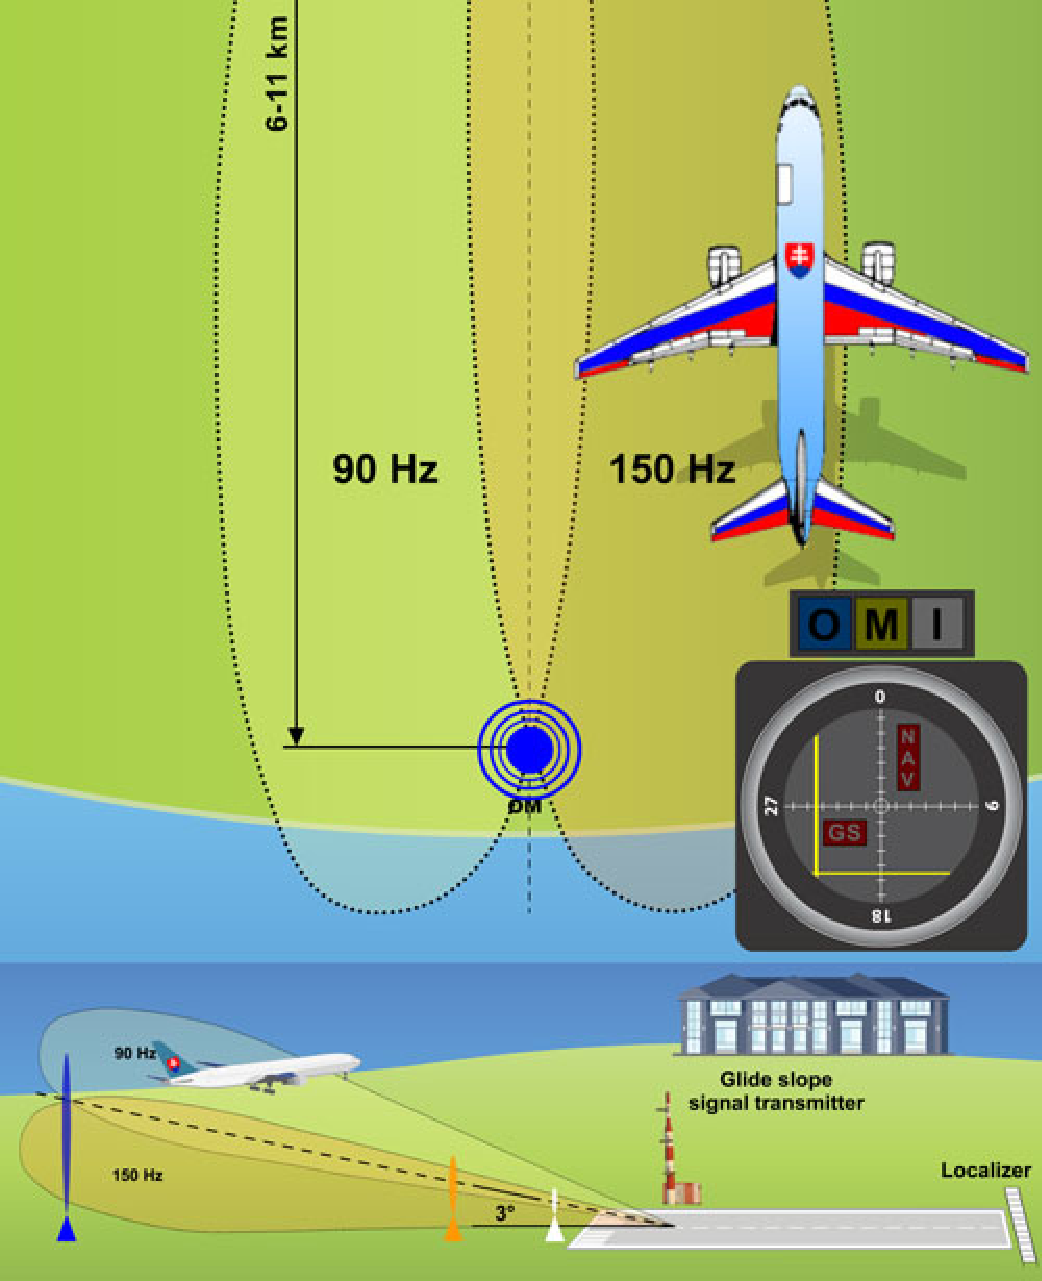
\includegraphics[height=7cm]{Figs/07_ILS1.pdf}}\hspace{4em}%
	\subfloat[飞机在左偏,高度低于标准下滑曲线时的机载仪表显示]{%
		\label{fig:08_ILS2}
		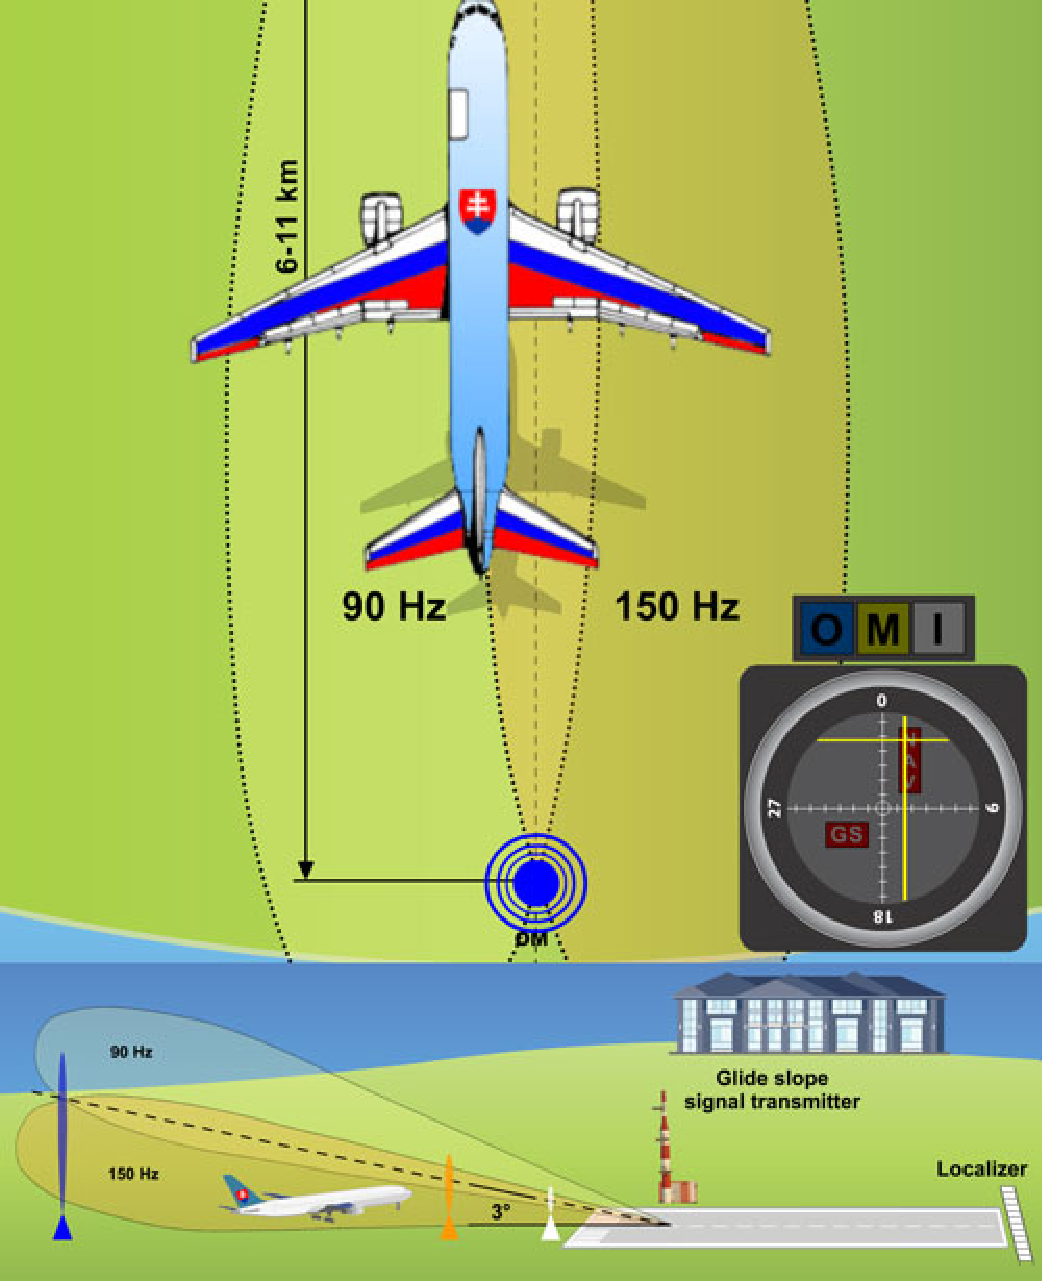
\includegraphics[height=7cm]{Figs/08_ILS2.pdf}}
	\caption{仪表着陆系统示意图}
	\label{fig:07_ILS}
\end{figure}

\subsubsection{雷达着陆系统}
随着二次大战对雷达在军事领域的广泛使用,美军在1943年研制了首套雷达着陆系统(GCA,Ground Control Approach),并于1946年拓展到民用领域。该系统通过地面引导雷达提供精确的位置信息,地面领航员根据雷达显示的下滑路径偏差与飞行员通话,进而操作飞机完成降落。随着技术发展,在雷达系统计算出下滑偏差后,可以根据飞机类型进行引导率计算,形成控制指令后反馈给飞机,协助飞行员或机载飞行系统完成下滑控制。这种方法也被称为“数据链+雷达”系统,至今仍然作为一种可靠的技术手段在航母和军用机场使用。

\subsubsection{微波着陆系统}
1978年,时间基准波束扫描技术(TRSB, Time Reference Scanning Beam)作为微波着陆技术的国际标准得到ICAO的认可。该系由地面方位台、仰角台、精密测距器和机载接收机组成。方位台和仰角台通过向空中发射扫描信号,机载接收机通过测量两次波束信号的时间间隔,得到飞机在空间的位置。但由于仪表着陆系统的广泛应用以及GNSS导航系统的迅猛发展,微波着陆技术的发展出现了一定的停滞。

\subsubsection{联合精密进近和着陆系统}
随着GPS和DGPS技术在美军的广泛应用,一套联合精密进近和着陆系统(JPALS)于2000年在地基完成测试实验。针对舰船本身和飞机都在运动,JPALS需采用双向的UHF数据链,将舰船测量到自身的GPS的位置,以及其摇摆、俯仰、偏航和向前运动的数据一并传给飞机,与此同时,飞机也将其GPS数据传回舰船。舰载的JPALS并不在意实际的位置误差,仅关注船和飞机偏离的量要相同,其着舰精度满足CAT III级别,纵向和横向精度控制在$1 \m$之内,能够完成航母着舰引导任务。在2005至2006年,JPALS开始替换现有的以雷达为基础的AN/SPN-46舰载精密进场着陆系统。这套系统还可用于舰上的空管,双向的数据链能使舰船以GPS跟踪、标注飞机方向。根据公布的合同要求,系统具备初始能力(IOC)时间为2019年,系统具备完全能力(FOC)时间为2030年。


\subsubsection{OPATS(Object Position and Tracking System)}
OPATS是瑞士RUAG宇航公司在1999年为瑞士空军开发研制的“目标定位跟踪系统”的简称,是一套基于激光技术的无人机自动着陆系统,用于瑞士空军的“巡逻兵”无人机。OPATS系统使用反射回来的激光信号对无人机进行跟踪,对目标无人机的动态位置进行连续测量跟踪,提供无人机在着陆阶段的可靠位置信息,并将高速更新的数据传输到地面站进行处,如图\ref{fig:15_OPTAS}所示。自1999年以来,RUAG已向全球范围内的众多用户交付了超过100套的OPATS系统。该系统的目标检测范围为35米至4000米,精度控制在1.5米。

\begin{figure}[htb]
	\centering%
	\subfloat[OPATS引导降落系统外场配置图]{%
		\label{fig:15_OPTAS1}
		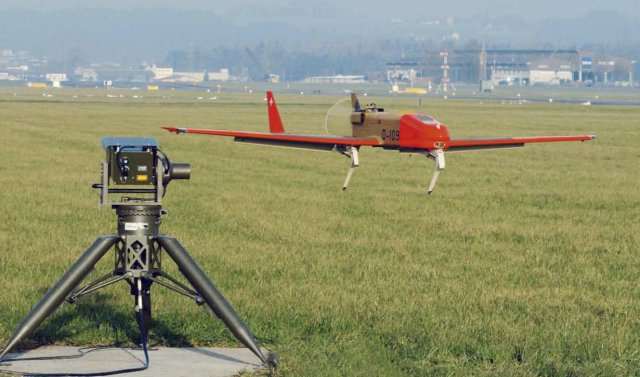
\includegraphics[height=4cm]{Figs/15_OPTAS1.jpg}}\hspace{4em}%
	\subfloat[OPATS引导降落系统框图]{%
		\label{fig:16_OPATS2}
		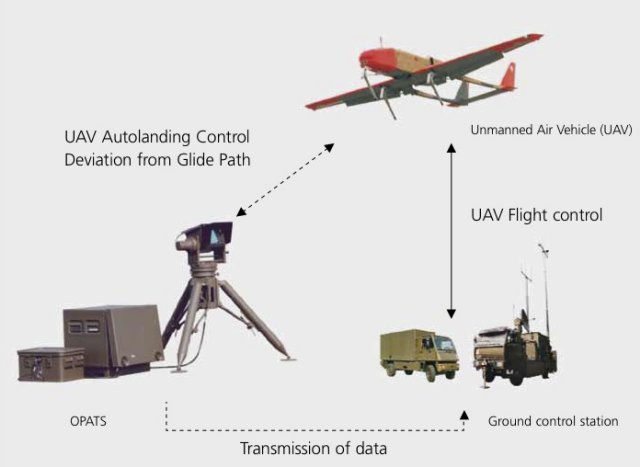
\includegraphics[height=4cm]{Figs/16_OPATS2.jpg}}
	\caption{OPTAS系统介绍}
	\label{fig:15_OPTAS}
\end{figure}


\subsubsection{光学引导系统}
光学助降系统主要依赖于“菲涅尔透镜”(Fresnel Lens)提供给飞行员相应的下滑曲线信息,以便飞行员操作飞机,即该引导系统是人在回路的引导方式。菲涅尔透镜有较好的聚焦性能,在同等焦距上由于传统球面透镜。由助降灯组和稳定平台组成,核心是位于中央的菲涅尔透镜和位于透镜两侧的水平基准灯。	舰载用的菲涅尔透镜系统(FLOLS, Fresenel Lens Optical Landing System)在传统的菲涅尔透镜基础上,将助降灯组与稳定平台结合。稳定平台的惯性系统可以检测舰船运动,使得射出的光束不受航母沉降摇摆的影响。在飞机进行着舰训练时,这套灯光组会释放出黄色、红色和橙色三种不同色彩光的下滑坡面,并以这三种光来界定高低位置。黄色光是高的下滑坡面,红色光是低的下滑坡面,橙色光是正确的下滑坡面。飞行员根据光所标定的位置在橙色光区域内下滑,就可以正确安全地着舰。


\subsubsection{基于UCARS的自主回收}
无人机通用自动回收系统(UAS Common Automatic Recovery System,UCARS)-V2系统(如图\ref{fig:29_UCARS})由内华达山脉公司(SNC)设计,为MQ-8B和MQ-8C火力侦察兵旋翼无人机的自主着陆提供引导控制。该系统是SNC的AN/UPN-51(V)无人机通用自动回收系统(UCARS)的改进型,并根据美军需求,拓展到其他型号的无人机引导降落,例如美国海军陆战队使用的先锋无人机。

该系统的主要传感器是毫米波雷达,该传感器也是军事和工业领域在引导无人机降落过程中使用最多的传感器质之一。毫米波雷达比普通的微波雷达体积更小,同时还具备波束窄和抗干扰能力强的特性;相比于红外传感器,毫米波雷达对于雨雾天气和灰尘的穿透性更强。UCARS系统主要由机载应答系统和舰载跟踪系统组成。跟踪传感器可以检测并计算无人机相对于期望降落点的位置信息,并向无人机提供降落平台的位置和运动状态数据,便于机载系统的导航和控制。目前UVARS系统有V2改进版,该版本使得无人机具备自主降落能力,减少了无人机飞行员的干预。此外,它还具备船舶运动稳定设备,以满足不同海况下的运行需求,该系统的引导控制精度在2.5厘米左右。系统的地基和舰载配置情况如图\ref{fig:29_UCARS}所示。 

\begin{figure}[htb]
	\centering%
	\subfloat[UCARS引导庞巴迪CL-227降落]{%
		\label{fig:29_UCARS1}
		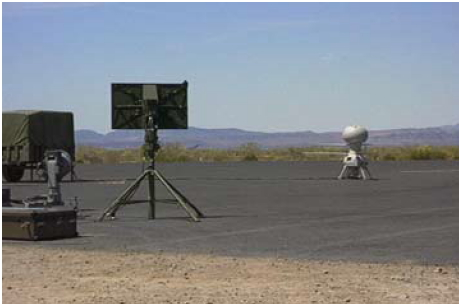
\includegraphics[height=4cm]{Figs/29_UCARS1.jpg}}\hspace{1em}%
	\subfloat[UCARS引导MQ-8B降落]{%
		\label{fig:30_UCARS2}
		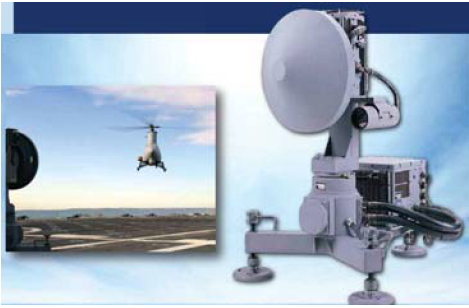
\includegraphics[height=4cm]{Figs/30_UCARS2.jpg}}
	\caption{无人机通用自动回收系统(UCARS)}
	\label{fig:29_UCARS}
\end{figure}

\subsubsection{无人机甲板起降引导系统}
法国DCNS公司开发的无人机直升机甲板起降引导系统(SADA\footnote{此处为法语缩写,Systèmed’Appontage et de Décollage Automatique})\cite{DCNS}使用红外传感器精确跟踪无人机,同时发出飞行指令调整航线直到确保无人机的“鱼叉”式着陆装置对准降落格栅的中心。2008年10,SADA成功将一架奥地利西贝尔公司研制的“坎姆考普特”(Camcopter)S-100无人直升机以自主模式降落在一艘正在地中海航行的法国海军驱逐舰“蒙特卡姆”号(Montcalm)上。该系统的引导控制精度约$30\ cm$。

\begin{figure}[!tb]   
	\centering	
	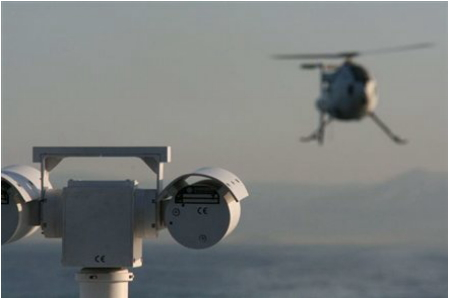
\includegraphics[width=0.5\textwidth]{Figs/24_SADA_Landing.jpg}
	\caption{SADA系统引导无人直升机着舰 }
	\label{fig:24_SADA_Landing}
\end{figure}


\subsubsection{基于D2AD自动甲板起降系统}
2011年,法国DCNS公司和Thales 公司完成无人机直升机在甲板自主降落(D2AD\footnote{此处为法语缩写,Démonstration d'un système d'appontage et d'atterrissage pour drones})的测试。此次海试使用法国海军“拉斐尔”级护卫舰和一架波音H-6U“小鸟”旋翼无人机,实验标志着 D2AD项目为期 4 年的技术验证成果。D2AD系统包括“飞行”部分和“地面”部分,“飞行”部分是无人机的指引标,“地面”部分在飞行甲板使用传感器进行船体运动预报,是无人机的引导站(如图\ref{fig:25_D2AD})。D2AD不依赖于任何卫星定位系统,能够保证垂直起降无人机在舰船上的安全使用。

\begin{figure}[htb]
	\centering%
	\subfloat[D2AD自主甲板降落系统]{%
		\label{fig:25_D2AD_1}
		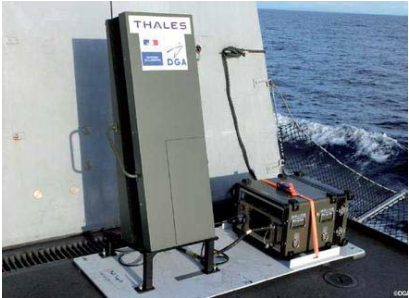
\includegraphics[height=4cm]{Figs/25_D2AD_1.jpg}}\hspace{0.1em}%
	\subfloat[H-6U“小鸟”旋翼无人机]{%
		\label{fig:26_D2AD_2}
		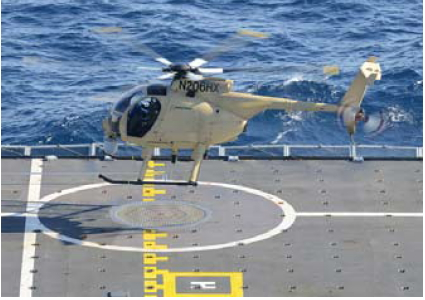
\includegraphics[height=4cm]{Figs/26_D2AD_2.jpg}}\hspace{0.1em}
	\subfloat[机载指引标]{%
		\label{fig:27_D2AD_3}
		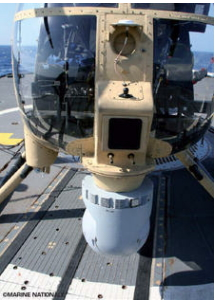
\includegraphics[height=4cm]{Figs/27_D2AD_3.jpg}}
	\caption{D2AD机载引导系统基本构成}
	\label{fig:25_D2AD}
\end{figure}

\subsubsection{基于DeckFinder的降落系统}
2013年6月,奥地利西贝尔电子设备公司的“坎姆考普特”S-100 无人直升机配装欧洲航宇防务集团(EADS)阿斯特里姆公司的“甲板发现者”(DeckFinder)区域定位系统,在一周的时间内完成了一系列旨在演示验证GPS干扰环境中无人机自动起飞与回收能力的飞行试验。“甲板发现者”系统\cite{Deckfinder}包括地面部分和机载部分,其中地面部分包括6台射频发射机,机载部分包括1台接收机。该系统的测距不依赖于GPS,可为航空器提供高精度的三维相对位置信息。根据公布的技术细节,该系统的工作范围约为$1.1\ km$,降落阶段精度优于$20\ cm$,工作频率不低于$15\ Hz$。
\begin{figure}[!tb]   
	\centering	
	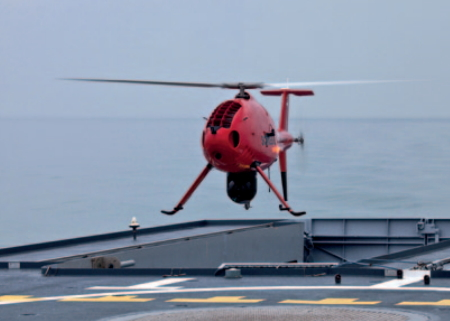
\includegraphics[width=0.5\textwidth]{Figs/28_Deckfinder.jpg}
	\caption{DeckFinder在GPS干扰环境下引导S-100无人机降落}
	\label{fig:28_Deckfinder}
\end{figure}

\subsubsection{基于JPALS的引导降落}
% X-47B
作为固定翼无人作战飞机,X-47B无人机面临着与其他无人机同样的难题:回收过程复杂。根据海军科技网站(Naval Technology)公布的消息\cite{X_47B_UCAS},X47-B的引导控制系统有较强的自主性,其导航系统主要由GPS和视觉系统组成。为提高智能化程度,X47-B还配备了光学系统、红外系统、SAR雷达(SAR, Synthetic Aperture Radar)、地面目标指示器(Ground mMving Tagret Indicator)和海面目标指示器(Maritime Moving Target Indicator)等设备。此外,在自主降落过程中,系统遵循预设的下降曲线对飞机进行引导和控制,操作员只是监视整个下降过程。虽然X-47B使用的具体引导降落方式没有公开,但通过公开视频和图像分析(如图\ref{fig:X47B_LandingOptical}所示),X-47B的自主着舰也应用了类似引导系统。

通过阅读相关资料并分析,该联合精确进场与着舰系统(JPALS)由处理、维修和监测系统,UHF数据链,惯性传感器和GPS传感器等组成,可以实现高可靠性和可用性。JPALS将与AN/TPX-42空中交通管制雷达、AN/SPN-46自动着舰系统、AN/SPN-41着舰辅助雷达、着舰信号官显示系统、改进型菲涅耳透镜光学着舰系统、航空数据管理和控制系统集成。2011年7月,F/A-18D“大黄蜂”战机在“艾森豪威尔”航空母舰上实现无人控制自主降落。

% ----- MQ-8B/C
2006年1月,MQ-8B完成了第一次在两栖登陆舰USS Nashville的舰载着陆,实验海域为Chesapeake Bay。2014年8月27日,MQ-8C“火力侦察兵”无人直升机在文图拉县海军基地完成着舰试验。

\subsection{无人机回收方式概述}
在X-47B无人机成功阻拦降落之前,世界各国在舰载无人机回收方面普遍采用的方法是:伞降回收、撞网回收、打捞回收和钩绳回收等。其中,撞网回收和钩绳回收对无人机回收控制精度提出更高要求,需要无人机自身或舰基系统具有较好的引导和控制能力。

\subsubsection{伞降回收}
伞降回收就是利用降落伞回收无人机。无人机从飞行状态到安全回收,整个过程自动完成,对操作人员要求较低。这种回收方式操作简单,是小型无人机回收的一种重要方式,适合对落点没有特殊要求的回收。采用轮式着陆的无人机也可使用伞降回收作为应急回收方案。采用水上伞降回收时,要考虑到无人机落入水中后对机身和内部设备的影响。

\subsubsection{撞网回收}
使用拦截网系统回收无人机是目前小型无人机较普遍采用的回收方式之一。无人机在降落阶段,通过降低高度和减小速度,撞向由弹性材料编制成的阻拦网。美国RQ-2“先锋”无人机和“银狐”无人机均采用
这类回收方式,如图\ref{fig:34_RQ2_Pioneer_Landing}所示。
\begin{figure}[!tb]   
	\centering	
	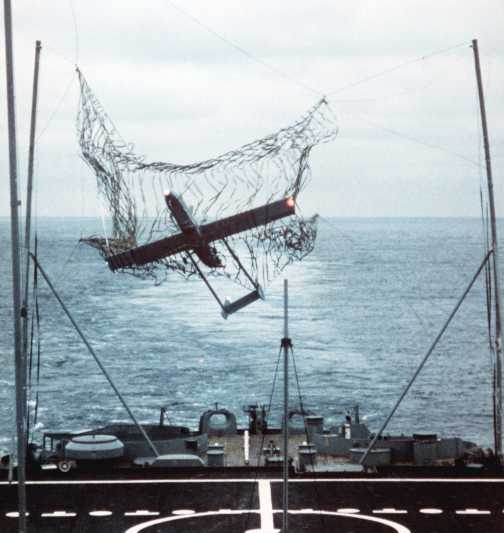
\includegraphics[width=0.4\textwidth]{Figs/34_RQ2_Pioneer_Landing.jpg}
	\caption{RQ-2在舰船完成撞网回收}
	\label{fig:34_RQ2_Pioneer_Landing}
\end{figure}

% Bat UAS
%翼展4.26 m、极长2.0 m、最大起飞重量159 kg、有效载荷34 kg。
%Shadow
%Poineer

\subsubsection{钩绳回收}
该回收方法使用垂直悬浮钢丝的天钩技术。钢丝可以自由的悬浮在吊杆上或者通过风筝把它升起,同时在无人机的翼尖上固定一个自锁的钩子。无人机进场时,径直地飞向钢丝,以便钢丝碰到其中一个机翼的前缘,然后滑向翼尖,通过钩子便可以把无人机锁住。由于航母的摆动幅度通常会限制为横摇2-3度,纵摇1-1.5度,而中小型船只稳定性要差得多,因此必须在横摇13度,纵摇5-6度的恶劣环境下,相比撞网回收,钩绳回收的引导控制需求更高,需要确保无人机在一米大小的回收窗口准确降落。

RQ-21A在2010年称为美国小型战术系统(Small Tactical Unmanned Aircraft System)项目的主力机型,该飞机具备陆基和海基起降能力,能够完成战术侦察、监视、目标指示(Reconnaissance, Surveillance and Target Acquisition,RSTA)功能,其模块化设计可快速替换不同传感器并完成部署。2014年7月,美国海军开始使用RQ-21A系统进行海上综合测试。该型无人机采用钩绳回收方式,如图\ref{fig:33_RQ21_Landing}所示。此外,“扫描鹰”无人机也采用此类方式回收,如图\ref{fig:35_Eagle_Scanner_Landing}所示。

\begin{figure}[htb]
	\centering%
	\subfloat[RQ-21在舰船回收]{%
		\label{fig:33_RQ21_Landing}
		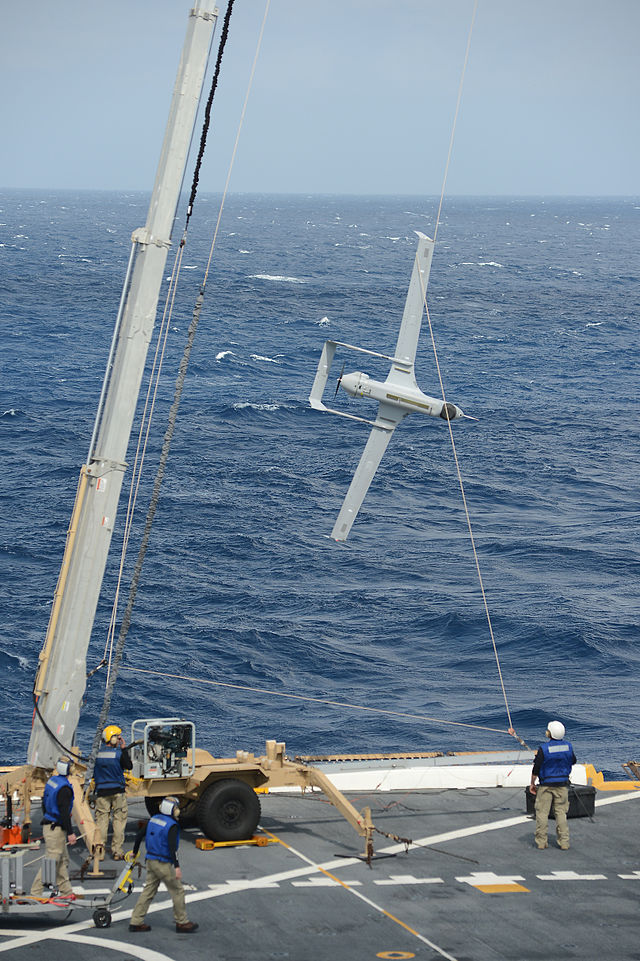
\includegraphics[height=6cm]{Figs/33_RQ21_Landing.jpg}}\hspace{0.1em}%
	\subfloat[“扫描鹰”无人机在舰船回收]{%
		\label{fig:35_Eagle_Scanner_Landing}
		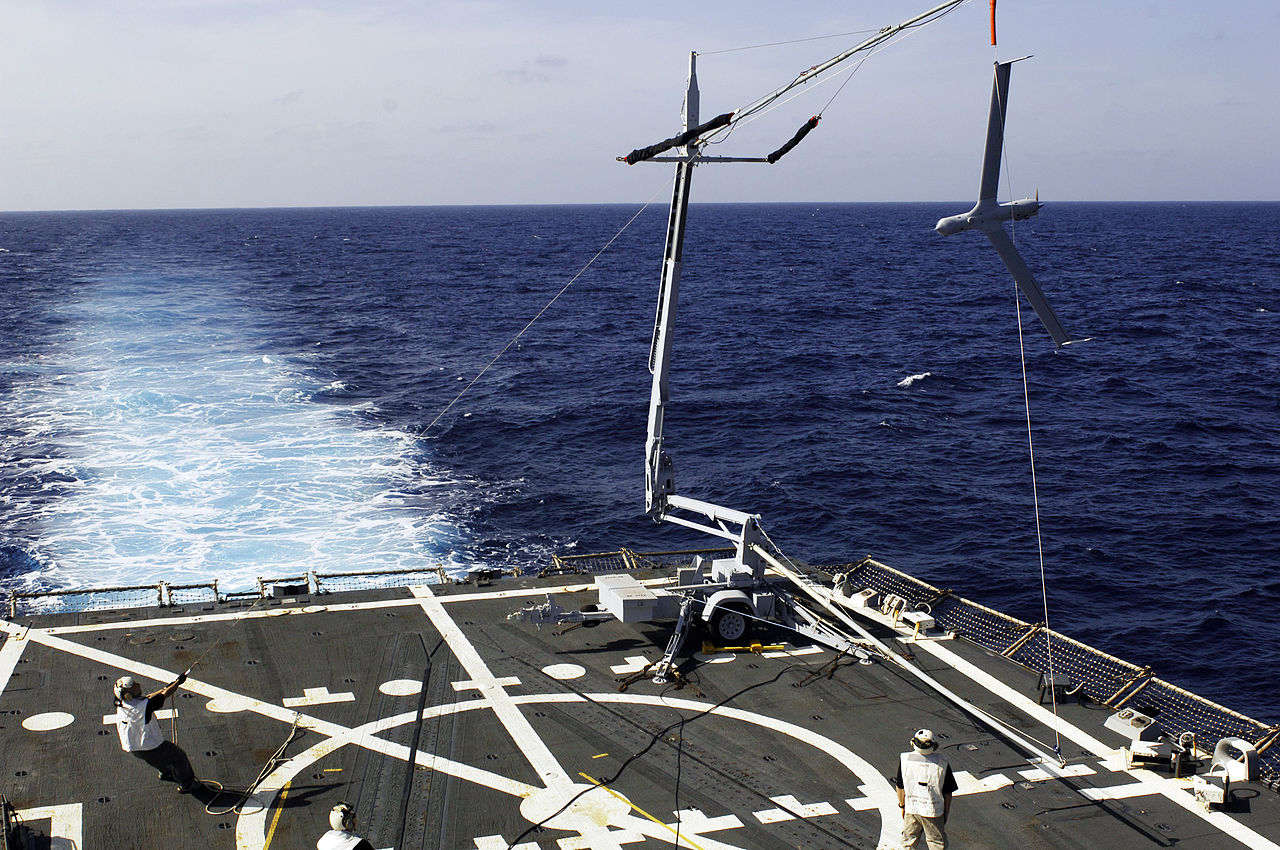
\includegraphics[height=6cm]{Figs/35_Eagle_Scanner_Landing.jpg}}\hspace{0.1em}
	\caption{采用钩绳回收方式的无人机}
	\label{fig:33_RQ21withScanner_Landing}
\end{figure}


\section{学术研究领域的无人机引导降落系统}
由于可见光摄像机成本低廉的特点,基于图像信息的无人机引导和控制在无人机实际应用中扮演十分重要的角色。例如,利用机载摄像机来完成感知规避任务\cite{mejias2010vision}、监视和跟踪任务\cite{campoy2009computer}\cite{mejias2006visual}、自主起飞和降落任务\cite{saripalli2002vision}、实时建图与定位任务(SLAM)\cite{weiss2011monocular}等。此外,通过图像信息对无人机自身位置和姿态进行估计也是今年来的研究重点和热点。比如在空中加油领域、无人机定点区域着陆等。2014年,针对视觉在无人机自主降落领域的研究现状,文章\cite{kong2014vision}系统总结了当前37个世界各地研究单位的工作,总结表格详见附录。本节只针部分内容进行概述。

\subsection{机载传感器引导降落系统} 

早在2003年,Shakernia\cite{shakernia2003vision}的博士论文中提出一种基于视觉的旋翼无人机(Yamaha R-50)的自主降落方案,该方案通过识别放置于六自由度运动平台上的合作标志完成自主降落(如图\ref{fig:chp01_06_shakernia_landing}所示)。其中,通过识别合作标志中的焦点,并使用Linear Two-view Motion Estimation, Non-linear Two-view Motion Estimation和Multi-view Planar Algorithm方法对飞机的位置和姿态进行估计。上述三种方法可以较好的解决特征点共面的飞机和位置姿态估计问题,通过仿真和户外试验,验证了系统的有效性和鲁棒性(位置偏差小于0.05米,角度偏差小于0.5°),但对于非合作目标的识别,不具备求解的通用性。

\begin{figure}[!tb]   
	\centering	
	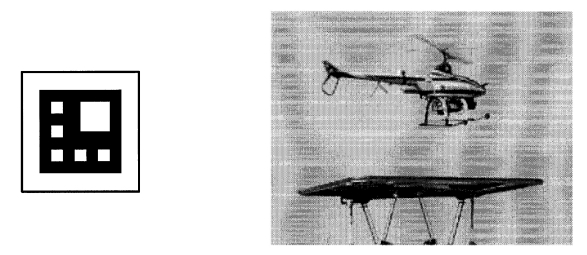
\includegraphics[width=\textwidth]{figs/chp01/chp01_06_shakernia_landing.pdf}
	\caption{基于合作标识的无人直升机自主降落系统}
	\label{fig:chp01_06_shakernia_landing}
\end{figure}


2009年,朱建明\cite{Zhu_Master_2009}对传统“H”形合作目标进行改进将“H”形图标的上端开口封住,改进后的图标能够克服“H”形图标缺乏有方向性的缺点,在地标图案分割的基础上,采用基于灰度变化的角点检测方法,提取合作标志的特征点。

2010年之后,该领域的研究逐渐增多。韩国科学技术院(Korea Advanced Institute of Science and Technology,KAIST)提出一种应用于小型无人机上的视觉引导着陆系统通过视觉引导无人机飞行至安装在地面上的红色圆拱形安全气袋中\cite{huh2010vision},原理如图\ref{fig:chp01_05_korea_landing}所示。
\begin{figure}[!tb]   
	\centering	
	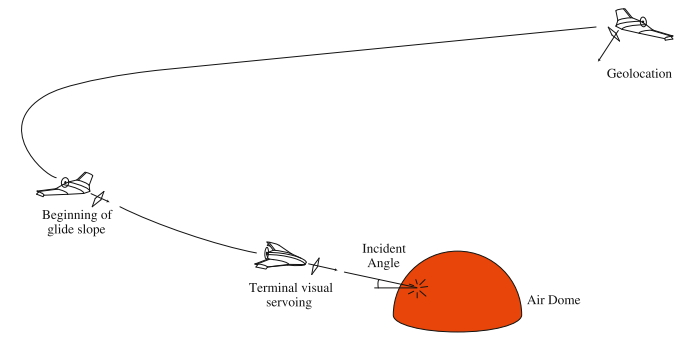
\includegraphics[width=\textwidth]{figs/chp01/chp01_05_korea_landing.pdf}
	\caption{基于红色标志物的无人机回收系统示意图}
	\label{fig:chp01_05_korea_landing}
\end{figure}

李宇\cite{Li_Master_2012}设计了一种由6个圆心已标识出来的红色圆圈组成的合作标志,通过基于仿射不变矩和SVM分类器实现着陆地标的识别,如图\ref{fig:chp01_04_six_circle_landing_pattern}所示。
\begin{figure}[!tb]   
	\centering	
	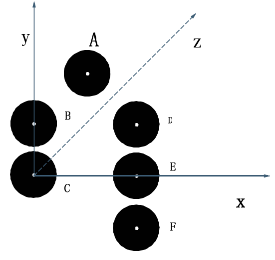
\includegraphics[width=0.4\textwidth]{figs/chp01/chp01_04_six_circle_landing_pattern.pdf}
	\caption{六个圆形合作标识}
	\label{fig:chp01_04_six_circle_landing_pattern}
\end{figure}

H. Jin Kim等人\cite{kim2013fully},针对小型固定翼无人机提出了一种基于机载视觉的撞网回收系统。该系统采用颜色分割和形态学等图像处理算法,通过机载摄像头对无人机回收网进行检测和识别;通过几何位置分析,判断无人机当前的方位信息,设计无人机引导率和控制率;地面控制系统可以向无人机发送控制命令并监测无人机的飞行状态。

德国宇航局在2015至2016年进行了HALE(High Altitude Long Endurance) UAV在运动汽车顶部回收的实验测试,该型号无人机的翼展为$3.3\ m$,最大起飞重量为$21.5\ kg$。该无人机在距离地面车辆$300\ m$左右的距离捕获地面移动车辆,随后地面移动车辆加速至合适的速度,满足无人机的回收需要。在回收过程中,无人机的引导方式主要通过机载摄像机对汽车顶部的合作标识(二维码)进行识别,进而实现相对位置的解算,完成自主降落\cite{Muskardin2016}。由于合作标识的尺寸和机载相机视场角的约束,无人机检测到地面目标点的距离较短,系统有效工作范围较小。
\begin{figure}[htb]
	\centering%
	\subfloat[无人机在回收末状态时,与汽车的速度保持相同]{%
		\label{fig:07_ILS1}
		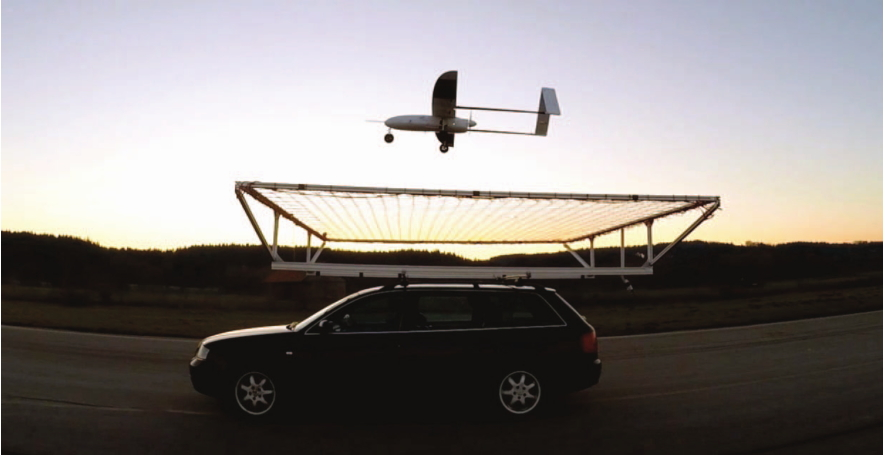
\includegraphics[height=3.5cm]{figs/chp01/chp01_01_DLR_Landing.pdf}}\hspace{0em}%
	\subfloat[机载传感器通过识别车顶的合作标识,实现相对位置的解算]{%
		\label{fig:08_ILS2}
		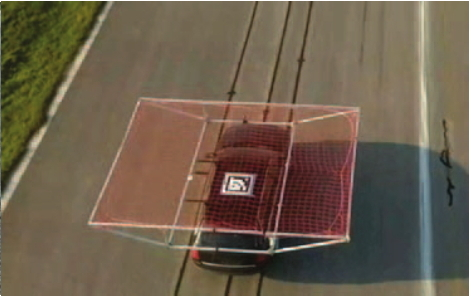
\includegraphics[height=3.5cm]{figs/chp01/chp01_02_DLR_Landing_with_tag.pdf}}
	\caption{德国宇航局车载无人机回收试验图}
	\label{fig:07_ILS}
\end{figure}

2016年5月,卡内基梅隆大学的研究者发布了最新无人直升机降落在海面移动平台\cite{Grocholsky2016}的工作。无人机上装载了长波红外传感器,该传感器适应雨雾天气,最远探测海面移动平台的距离为1.2海里(约2.22公里)。无人机从500米开始,对海面移动平台进行位置估计,并逐渐靠近该平台。在距离195米左右时,机载可见光传感器可以识别位于降落平台的合作标识,并具备对该平台姿态进一步估计的能力,其识别效果如图\ref{fig:chp01_03_CMU_Sea_Landing}所示。在最后50米的距离,激光传感器通过对甲板的三维空间扫描,实现厘米级的位置解算精度。

\begin{figure}[htb]   
	\centering
	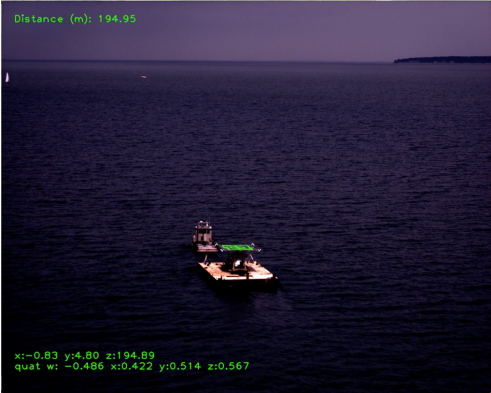
\includegraphics[width=0.6\textwidth]{figs/chp01/chp01_03_CMU_Sea_Landing.pdf}
	\caption{卡内基梅陇大学直升机机载视觉传感器在降落过程中的对降落目标位置和姿态的解算}
	\label{fig:chp01_03_CMU_Sea_Landing}
\end{figure}

此外,通过机载传感器直接识别机场跑道,也可以视为一种基于合作标识的降落方法。德国宇航中心DLR飞行控制研究所提出了一种利用可见光、红外或雷达图像中的跑道信息估计固定翼飞机的相对位置的方法,并在其研制的ESVS(Enhanced and Synthetic Vision)平台上得到验证\cite{doehler2003robust}。

\subsection{地基传感器引导降落系统} 

用于户外的地基引导系统并不常见,国防科技大学在2011年,提出一种地基引导系统\cite{Ding_master_2011},该系统通过地面摄像机识别无人机上悬挂的红外标记,完成对无人机的引导降落。在目标无人机沿下滑曲线下降至$400\ m$左右的距离时,引导系统开始工作,此时的无人机高度约为$50\ m$;在距离相机$50\ m$距离时,系统的高度分辨率为$0.032\ m$,水平分辨率为$0.26\ m$。该系统的排布如图\ref{fig:chp01_07_ding_master}所示。

\begin{figure}[htb]   
	\centering
	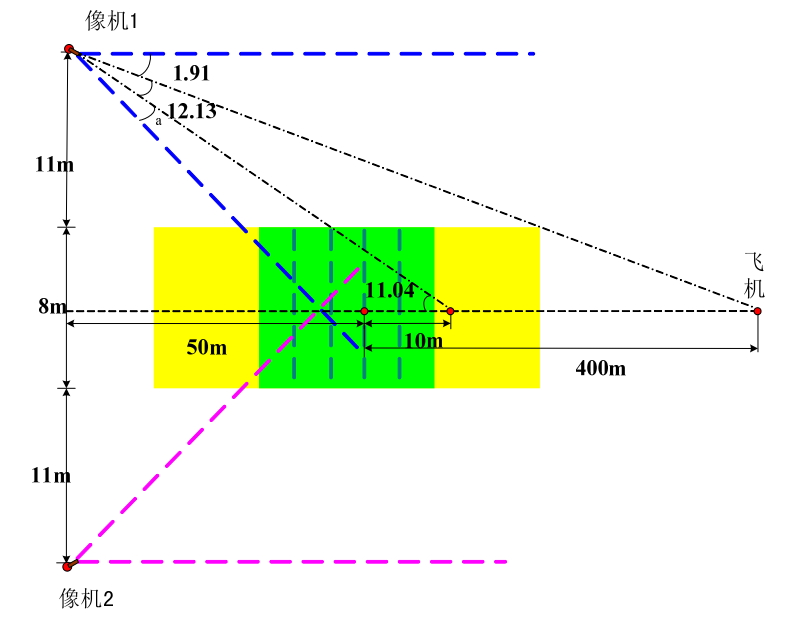
\includegraphics[width=0.6\textwidth]{figs/chp01/chp01_07_ding_master.pdf}
	\caption{地面引导系统排布示意图}
	\label{fig:chp01_07_ding_master}
\end{figure}

此外,该研究组还提出了采用多台固定焦距摄像机分区域接力测量的方案如图\ref{fig:chp01_08_gui_doctor}所示\cite{gui_doctor_2013}。视觉引导系统由三组摄像机选取不同的焦距,分别观测远场、中场和近场区域,保证相邻两组摄像机视场有一定的重叠区域,并覆盖无人机的下降区域。

\begin{figure}[htb]   
	\centering
	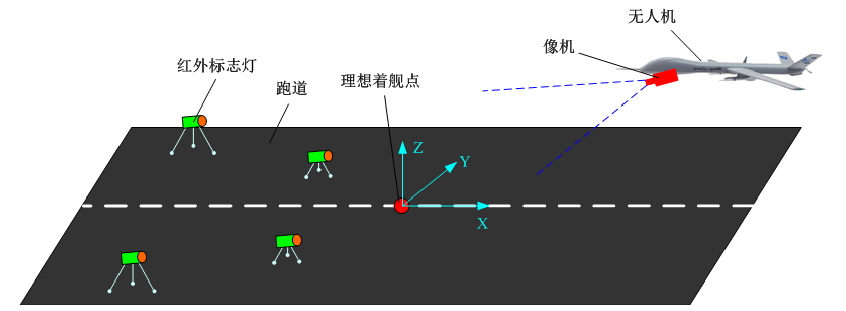
\includegraphics[width=0.6\textwidth]{figs/chp01/chp01_08_gui_doctor.pdf}
	\caption{地基多相机引导系统示意图}
	\label{fig:chp01_08_gui_doctor}
\end{figure}

文献\cite{Garcia-Pardo2002}给出了一种基于步进电机和网络摄像头结合的引导设备,可以对微小型无人机进行跟踪,但其视场角受到步进电机的约束。Martinez\cite{Martinez2010}提出了一种三目摄像机系统,如图\ref{fig:chp01_09_three_ground_landing}所示,该系统可以检测无人机的特征点,得到位置信息,但由于构型限制,该系统只适用于旋翼直升机的降落。美国斯坦福大学(Stanford University)\cite{Saripalli2003}使用两个或以上的相机得到了距离$40\ m$外,位置误差约$25\ cm$的视觉系统,但文献中没有具体描述系统的具体结构。日本千叶大学(Chiba University)的研究者\cite{PEBRIANTI2010}使用利用Bumblebee立体视觉传感器,成功将一架四悬翼从$6\ m$的高度引导降落。

\begin{figure}[htb]   
	\centering
	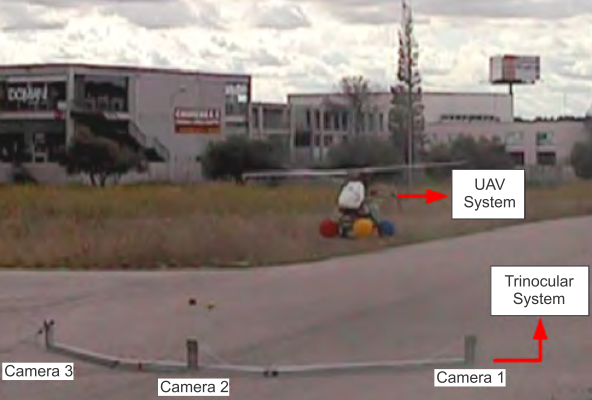
\includegraphics[width=0.7\textwidth]{figs/chp01/chp01_09_three_ground_landing.pdf}
	\caption{地面引导系统排布示意图}
	\label{fig:chp01_09_three_ground_landing}
\end{figure}

\section{本文的主要工作、贡献和结构}
本文瞄准固定翼无人机着舰回收的实际需求,重点研究着舰引导控制的系统架构、机理建模、关键算法与综合验证,主要工作和贡献如下:

(1)提出一种舰基通用的多传感器无人机回收引导系统。该系统主要有两个独立引导单元组成,每个引导单元配备一个二自由度转台和可见光相机、红外相机等多个传感器。两个独立引导单元的排布可以根据目标无人机的大小和检测距离进行优化配置。本文针对该系统独立分布在跑道两侧的特点,通过对目标位置解算理论推导、误差分析和实验验证,证明了在无人机降落过程中,使用上述引导系统的可行性。

(2)提出检测-跟踪-学习相融合的无人机降落过程中实时目标跟踪和位置解算框架。针对引导无人机降落过程中,无人机目标尺度快速变化问题,通过改进基于形态学滤波的图像预处理方法,TLD目标跟踪框架和基于主动轮廓的目标位置修正方法,结合转台运动位置和无人机运动的估计,能够准确解算出无人机在降落过程中相对于舰船的位置信息,满足无人机引导和控制系统的需要。

(3)设计基于非线性模型预测控制(NMPC)和总能量控制(TESC)的无人机着舰控制系统。由于无人机机载设备运算能力的约束,本文设计了内环控制器和外环控制器来实现无人机的自主降落。其中内环控制器由PI和PD控制器组成,完成对无人机姿态的控制;外环控制器由非线性模型预测控制器(NMPC)和总能量控制器(TESC)组成,针对基于Dubins Path生成的降落曲线进行跟踪。

(4)设计并实现无人机舰载着舰系统仿真环境并进行户外实验验证。本文基于机器人操作系统(Robot Operating System,ROS)和Gazebo仿真环境构建了无人机舰载着陆软件在回路仿真系统(SITL)和硬件在回路仿真系统(HIL)。该仿真环境能够满足上述算法的验证需求。通过二自由度转台与多传感器的组合配置,实现在地面机场和水面环境对小型和中型固定翼无人机的引导和自主降落。

本文各个章节的结构图如图\ref{fig:chp01_10_thesis_structure}所示。
\begin{figure}[!h]   
	\centering	
	\includegraphics[width=\textwidth]{figs/chp01/chp01_10_thesis_structure.pdf}
	\caption{本文的组织结构图}
	\label{fig:chp01_10_thesis_structure}
\end{figure}

	\chapter{无人机着舰环境数学建模}
\label{chap:main}
无人机着舰的过程设计到无人机系统和舰船系统两大部分,因此为了研究这两部分直接的关系,必须对降落过程进行适当的数学模型\cite{beardsmall},以利于对无人机控制和引导系统进行数学仿真和物理实验。

\section{无人机系统坐标系定义}


\subsection{系统惯性坐标系}
系统惯性坐标系(Inertial Frame,$\mathcal{F}^i$),该坐标系一般定义位于地球表面的一点,三个轴的方向$(\mathbf{i}^i, \mathbf{j}^i,\mathbf{k}^i)$与地球的北向、动向和指向地心方向相同,即NED坐标系。通常该坐标系定义为飞机的起飞点或降落点,本文中我们选用无人机被舰船引导系统捕获时,舰船的此刻所在的点为原点,如图\ref{fig:chp02_01_sys_interial_frame}所示。
\begin{figure}[htb]   
	\centering
	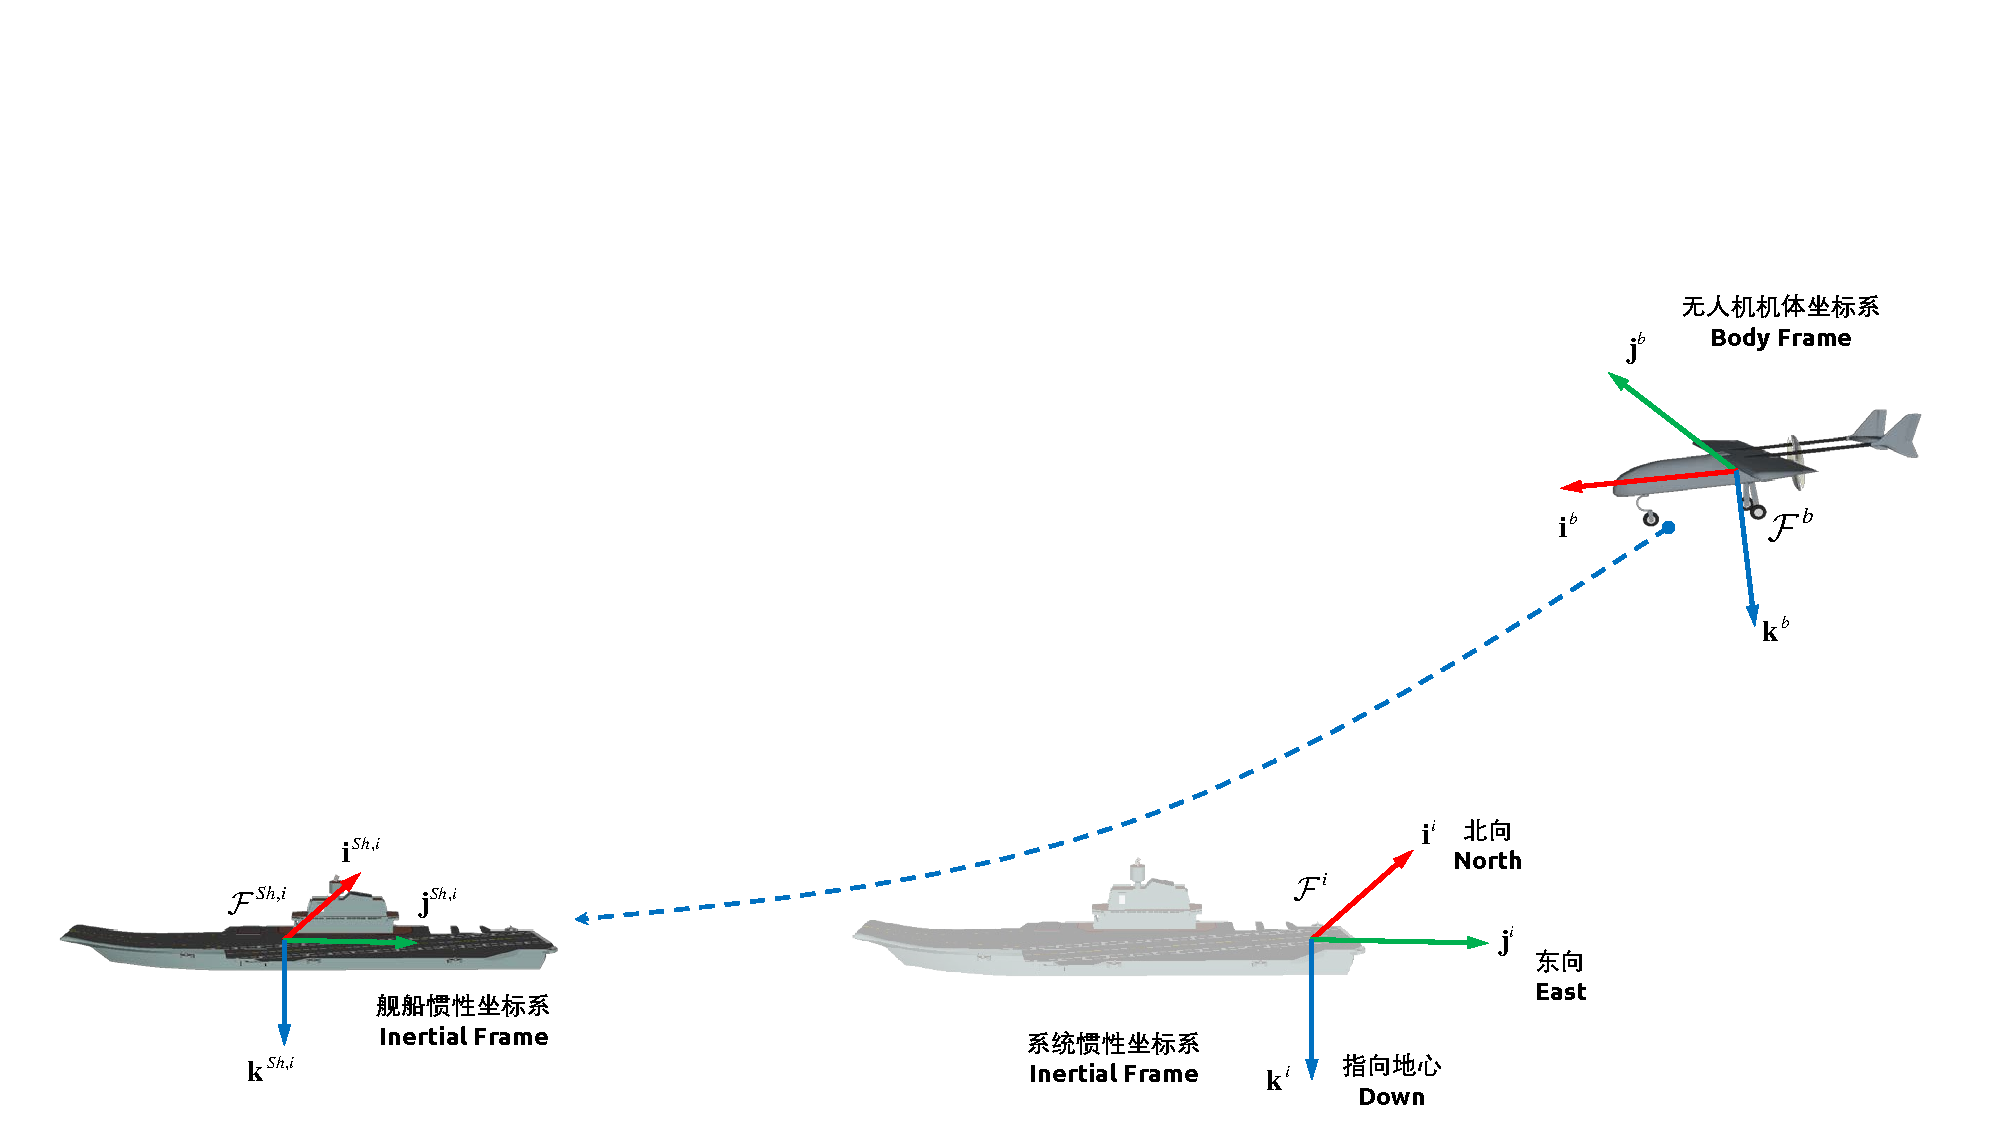
\includegraphics[width=\textwidth]{figs/chp02/chp02_01_sys_interial_frame.pdf}
	\caption{系统惯性坐标系}
	\label{fig:chp02_01_sys_interial_frame}
\end{figure}

\subsection{无人机惯性坐标系}
无人机惯性坐标系($\mathcal{F}^v$,Vehicle Inertial Frame),该坐标系的原点位于飞机的重心,三轴方向与系统坐标系平行。

\begin{figure}[htb]   
	\centering
	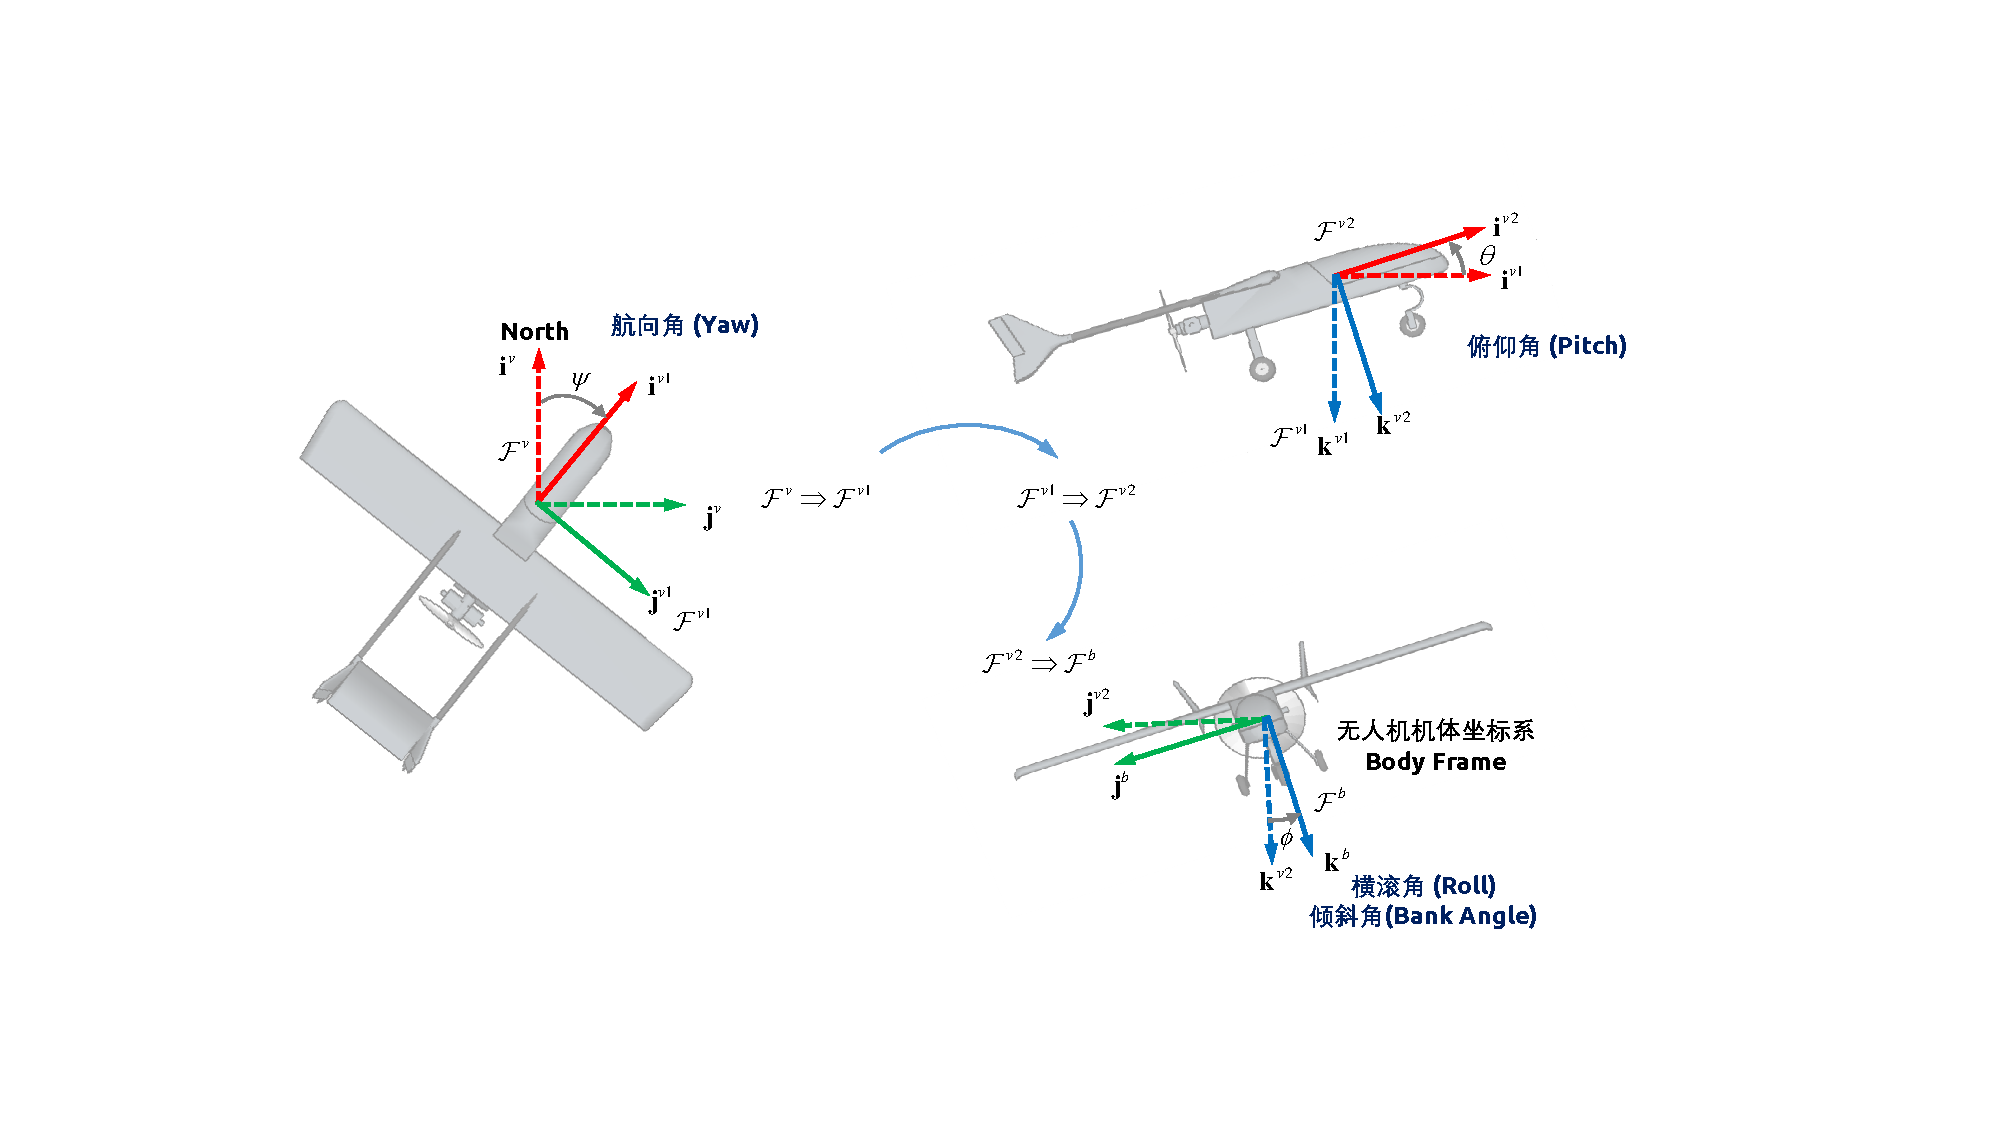
\includegraphics[width=\textwidth]{figs/chp02/chp02_02_uav_rpy.pdf}
	\caption{无人机机体坐标系与横滚角、俯仰角和偏航角定义}
	\label{fig:chp02_02_uav_rpy}
\end{figure}

无人机第一惯性辅助坐标系($\mathcal{F}^{v1}$ ),该坐标系绕无人机惯性坐标系$\mathbf{k}^v$轴按右手规则旋转得到,其中旋转角度定义为$\psi$,即偏航角(Yaw Angle)。

无人机第二惯性辅助坐标系($\mathcal{F}^{v2}$),该坐标系过绕人机第一惯性辅助坐标系$\mathbf{j}^{v1}$轴按右手规则旋转旋转得到,其旋转角度定义为$\theta$,即俯仰角(Pitch Angle)。

无人机机体坐标系($\mathcal{F}^b$,Body Frame ),该坐标系绕无人机第二惯性辅助坐标系$\mathbf{i}^{v2}$轴按右手规则旋转旋转得到,其旋转角度定义为$\phi$,即横滚角(Roll Angle),有时该角度也被称为倾斜角(Bank Angle)。上述四个坐标系之间的转换关系如图\ref{fig:chp02_02_uav_rpy}所示。

根据上述四个坐标系的几何关系,可以得到由机体惯性坐标系$\mathcal{F}^v$转换到机体坐标系$\mathcal{F}^b$的转换矩阵为
\begin{multline}
\mathcal{R}_v^b(\phi, \theta, \psi) =\mathcal{R}_{v2}^b(\phi)\mathcal{R}_{v1}^{v2}(\theta)\mathcal{R}_v^{v1}(\psi) \\
=\begin{bmatrix}
\cos \theta \cos \psi                             & \cos\theta \sin\psi                               & -\sin\theta         \\
-\cos\phi \sin\psi + \sin\phi \sin\theta \cos\psi & \cos\phi \cos\psi + \sin\phi \sin\theta\sin\psi   & \sin\phi \cos\theta \\
\sin\phi \sin\psi + \cos\phi \sin\theta \cos\psi  & -\sin\phi \cos\psi + \cos\phi \sin\theta \sin\psi & \cos\phi \cos\theta
\end{bmatrix}
\end{multline}


机体坐标系$\mathcal{F}^b$转换到稳定坐标系$\mathcal{F}^s$的转换矩阵为
\begin{equation} 
\mathcal{R}_b^s(\alpha) = \begin{bmatrix}
\cos \alpha                             & 0                               & \sin \alpha         \\
0 & 1   &0 \\
-\sin \alpha   & 0 & \cos \alpha
\end{bmatrix}
\end{equation}

稳定坐标系$\mathcal{F}^s$转换为风坐标系$\mathcal{F}^w$的转换矩阵为
\begin{equation} 
\mathcal{R}_s^w(\beta) = \begin{bmatrix} \sin \beta  & \cos \beta  &  0      \\  - \sin \beta & \cos \beta   &0 \\  0   & 0 &1  \end{bmatrix}
\end{equation}

风坐标系$\mathcal{F}^w$转换为机体坐标系$\mathcal{F}^b$转换矩阵为

\begin{equation} 
\mathcal{R}_w^b (\alpha,\beta) = \begin{bmatrix} \cos \beta \cos \alpha & - \sin \beta \cos \alpha  & - \sin \alpha      \\	 \sin \beta & \cos \beta   & 0 \\	\cos \beta   & -\sin \beta \sin \alpha & \cos \alpha \end{bmatrix}
\end{equation}

\subsection{无人机风向坐标系}
无人机风向坐标系($\mathcal{F}^w$,Wind Frame),该坐标系的$\mathbf{i}^w$轴与风速方向相同,可以通过旋转稳定坐标系的$\mathbf{k}^s$轴$\beta$角度得到,该角度$\beta$被定义为侧滑角。无人机攻角和侧滑角的定义如图\ref{fig:chp02_03_uav_aoa_bank}所示。
\begin{figure}[htb]   
	\centering
	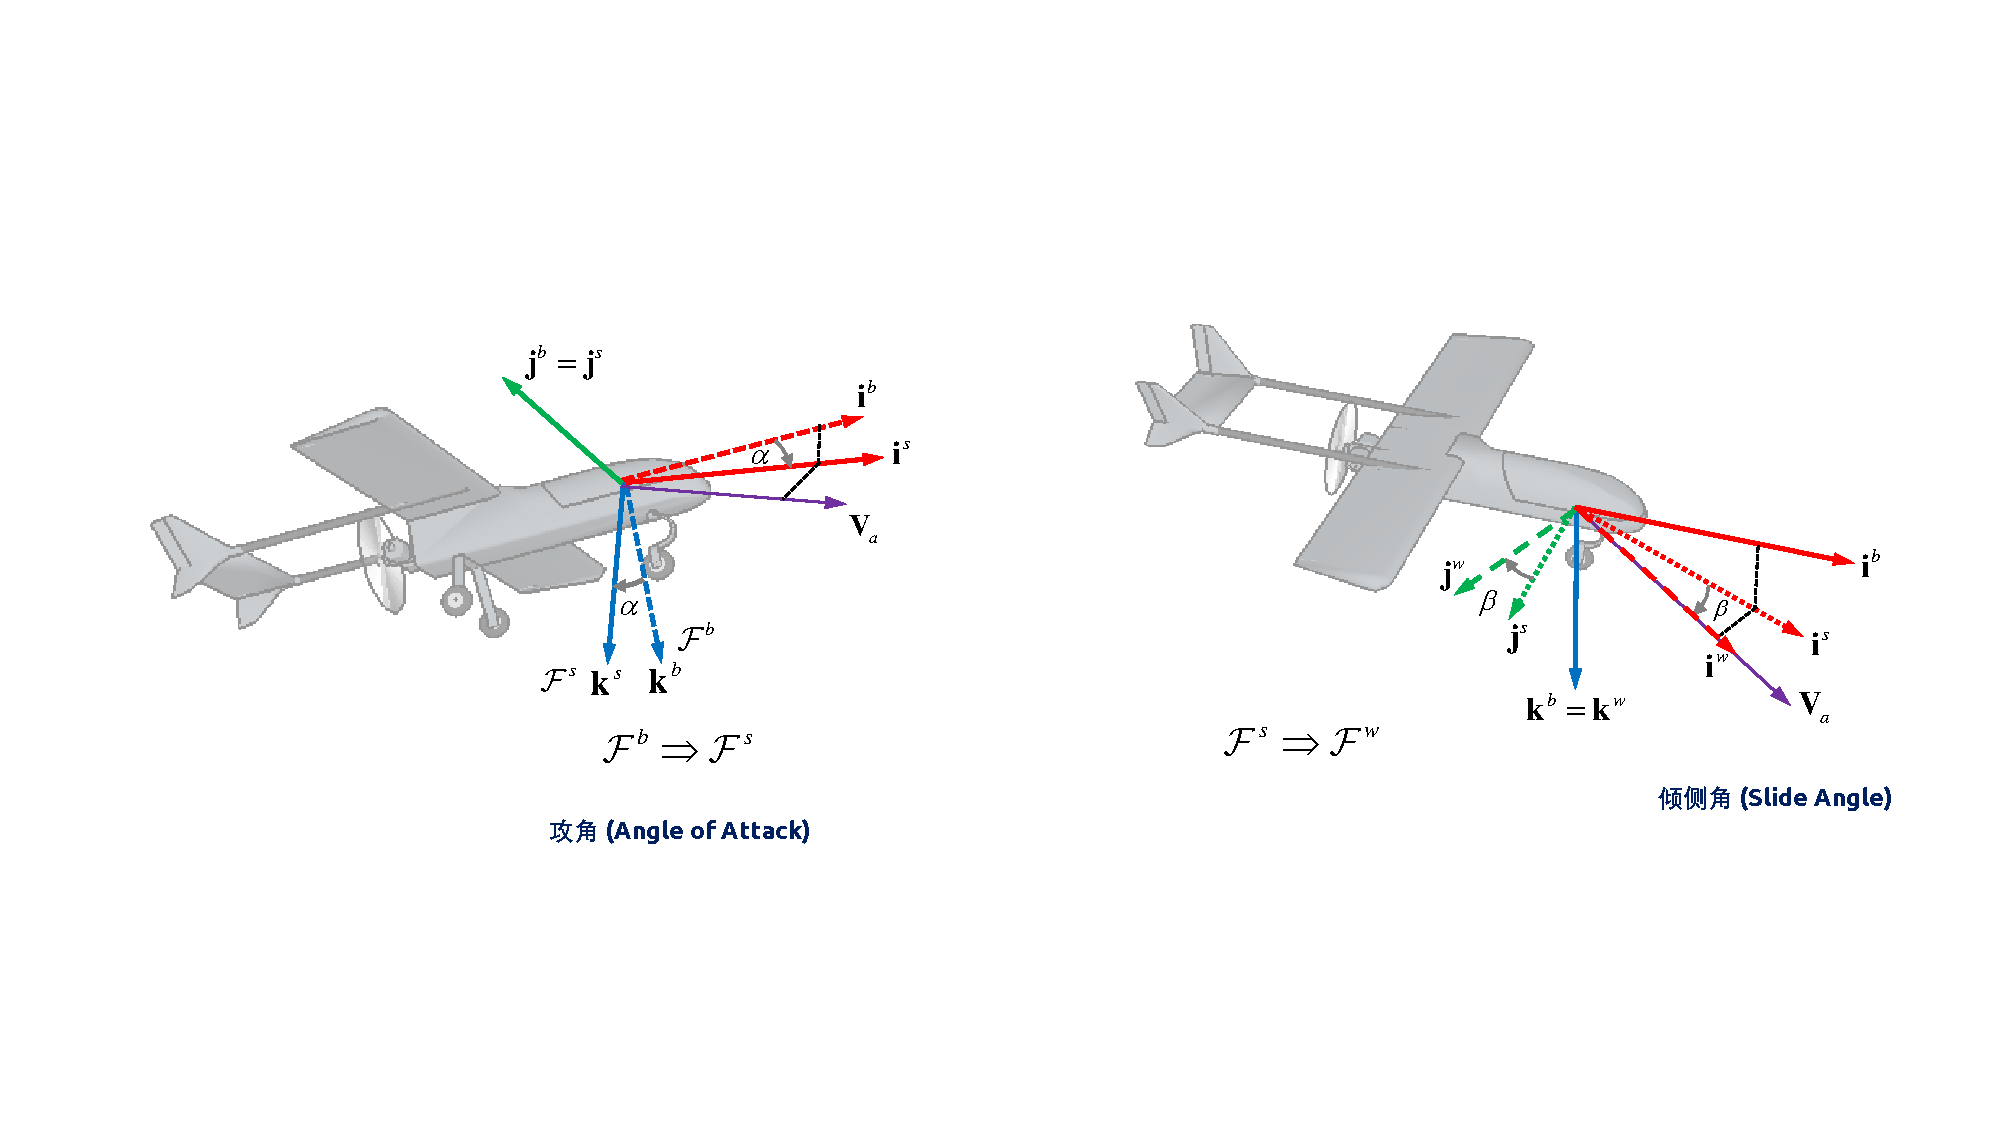
\includegraphics[width=\textwidth]{figs/chp02/chp02_03_uav_aoa_bank.pdf}
	\caption{无人机稳定坐标系与攻角、侧滑角定义}
	\label{fig:chp02_03_uav_aoa_bank}
\end{figure}

\subsection{无人机稳定坐标系}
无人机稳定坐标系($\mathcal{F}^s$,Stability Frame),该坐标系绕无人机机体坐标系$\mathbf{j}^b$按左手规则旋转得到,该坐标系表达如图\ref{fig:chp02_03_uav_aoa_bank}。其中,定义无人机相对于机体周边空气的速度向量为$\mathbf{V}_a$,其大小为$V_a$。为使机翼产生升力,机翼与风速的夹角必须为正,该角度定义为攻角。这里使用左手系的原因是为更方便的定义定义攻角$\alpha$的正负,即沿稳定坐标系$\mathbf{j^s}$按右手系转动到机体坐标系的角度为正。稳定坐标系的$\mathbf{i}^s$轴与空速向量$\mathbf{V}_a$在$\mathbf{i}^b$-$\mathbf{k}^b$的投影方向平行。

定义$\mathbf{V}_a$为空速(Airspeed),即无人机相对于周边流体的速度。
该向量在风坐标系$\mathcal{F}^w$的表达为
\begin{equation} 
\mathbf{V}_a^w=\begin{bmatrix} V_a \\ 0 \\ 0 \end{bmatrix}
\end{equation}
该向量在机体坐标系$\mathcal{F}^b$的表达为
\begin{equation} 
\mathbf{V}_a^b = \begin{bmatrix} u_r \\ v_r \\ w_r \end{bmatrix}
\end{equation}

$\mathbf{V}_g$定义为地速(Ground Speed),即无人机相对于系统惯性系的速度
无人机相对于惯性系的速度该向量在机体坐标系$\mathcal{F}^b$的表达为
\begin{equation}
\mathbf{V}_g^b=\begin{bmatrix} u \\ v \\w \end{bmatrix}
\end{equation}

$\mathbf{V}_w$定义为风速(Wind Speed),即风相对于系统惯性系的速度。
风速在机体坐标系$\mathcal{F}^b$的表达为
\begin{equation}
\mathbf{V}_w^b=\begin{bmatrix} u_w \\ v_w \\w_w \end{bmatrix} \\
=\mathcal{R}_v^b(\phi, \theta, \psi) \begin{bmatrix} w_n \\ w_e \\ w_d \end{bmatrix}
\end{equation}
其中$(w_n, w_e, w_d)$是风速在无人机惯性坐标系的表达。
上述三个速度直接的关系为
\begin{equation}
\mathbf{V}_a = \mathbf{V}_b - \mathbf{V}_w
\end{equation}

上述三个关系的表达如图\ref{fig:chp02_04_uav_wind_frame}所示,根据上述关系,可以得到风速在机体坐标系的另一个表达
\begin{equation}
\mathbf{V}_a^b  = \begin{bmatrix} u_r \\ v_r \\ w_r \end{bmatrix} =   \begin{bmatrix} u - u_w \\ v - v_w \\ w- w_w \end{bmatrix}
\end{equation}
根据风坐标系$\mathcal{F}^w$与$\mathcal{F}^b$机体坐标系的转换关系,风速在机体坐标系还可以表达为
\begin{equation}
\mathbf{V}_a^b  = \begin{bmatrix} u_r \\ v_r \\ w_r \end{bmatrix} \\
=  \mathcal{R}_w^b \begin{bmatrix} V_a \\ 0 \\ 0 \end{bmatrix} \\
=  \begin{bmatrix}	\cos \beta \cos \alpha & - \sin \beta \cos \alpha  & - \sin \alpha      \\	 \sin \beta & \cos \beta   & 0 \\ 	\cos \beta   & -\sin \beta \sin \alpha & \cos \alpha \end{bmatrix} \begin{bmatrix} V_a \\ 0 \\ 0 \end{bmatrix}
\end{equation}
由此可以得到上式更简便的表达
\begin{equation}
\begin{bmatrix} u_r \\ v_r \\ w_r \end{bmatrix}  = {V}_a \begin{bmatrix} \cos \alpha \cos \beta \\ \sin \beta  \\ \sin \alpha \cos \beta \end{bmatrix}
\end{equation}
注意,此处的$V_a$是风速向量的标量。

在已知风速相对于机体坐标系的向量表达时,可以进一步得到风速、攻角和侧滑角的计算
\begin{align}
V_a &= \sqrt{(u_r)^2+(v_r)^2+(w_r)^2} \\
\alpha &=  \tan^{-1}\frac{w_r}{u_r}  \\
\beta  &=  \sin^{-1} \big( \frac{u_r}{\sqrt{(u_r)^2+(v_r)^2+(w_r)^2}} \big)
\end{align}

\begin{figure}[htb]   
	\centering
	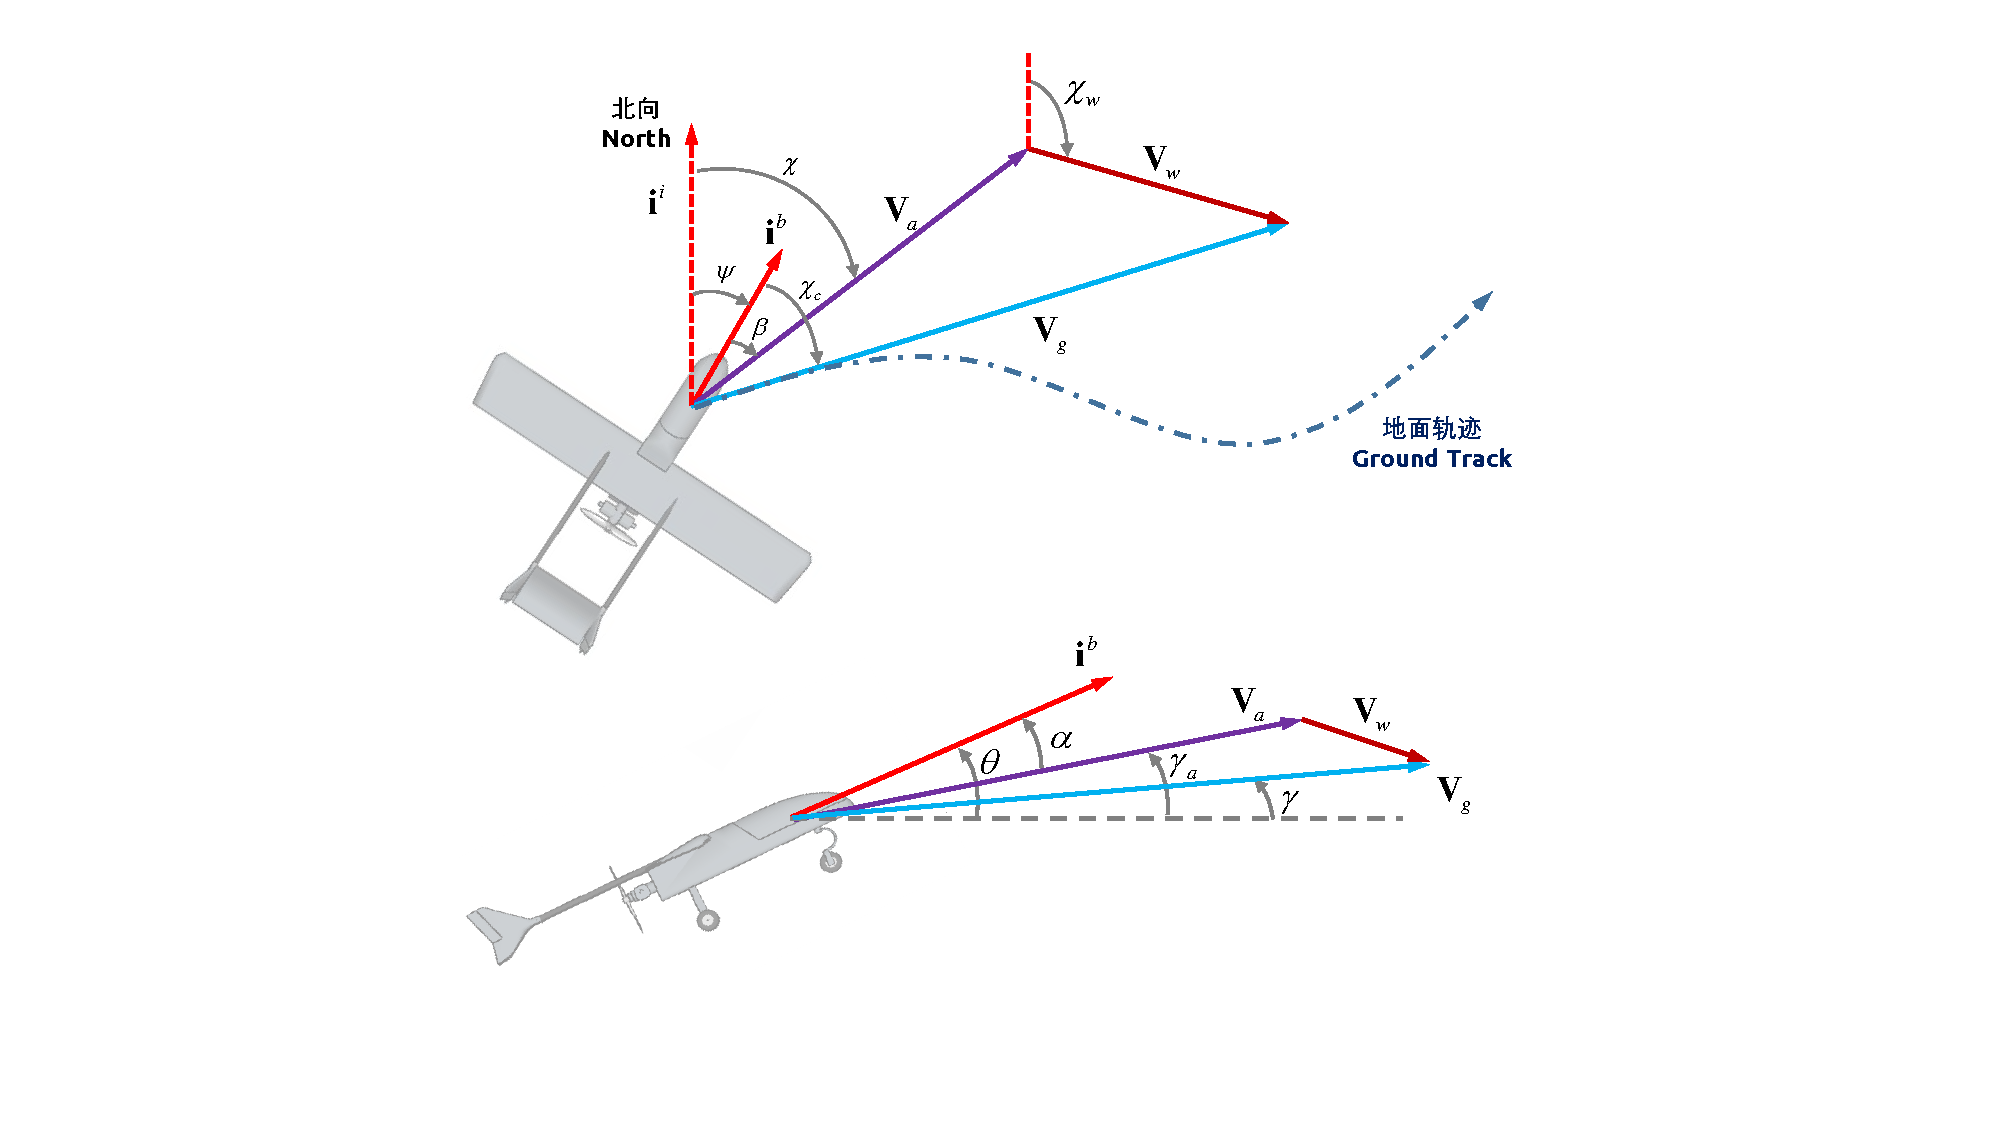
\includegraphics[width=0.8\textwidth]{figs/chp02/chp02_04_uav_wind_frame.pdf}
	\caption{无人机地速、风速和空速三角形}
	\label{fig:chp02_04_uav_wind_frame}
\end{figure}

 




\section{无人机系统运动学和动力学分析}
\subsection{三维空间向量微分}
假设在机体坐标系$\mathcal{F}^b$存在一个运动的向量$\mathbf{p}$,如图\ref{fig:chp02_06_vector_rotation}所示,该向量的数学表达为 
\begin{equation}
\mathbf{p }= p_x \mathbf{i}^b +  p_y \mathbf{j}^b +  p_z \mathbf{k}^b
\end{equation}
\begin{figure}[htb]   
	\centering
	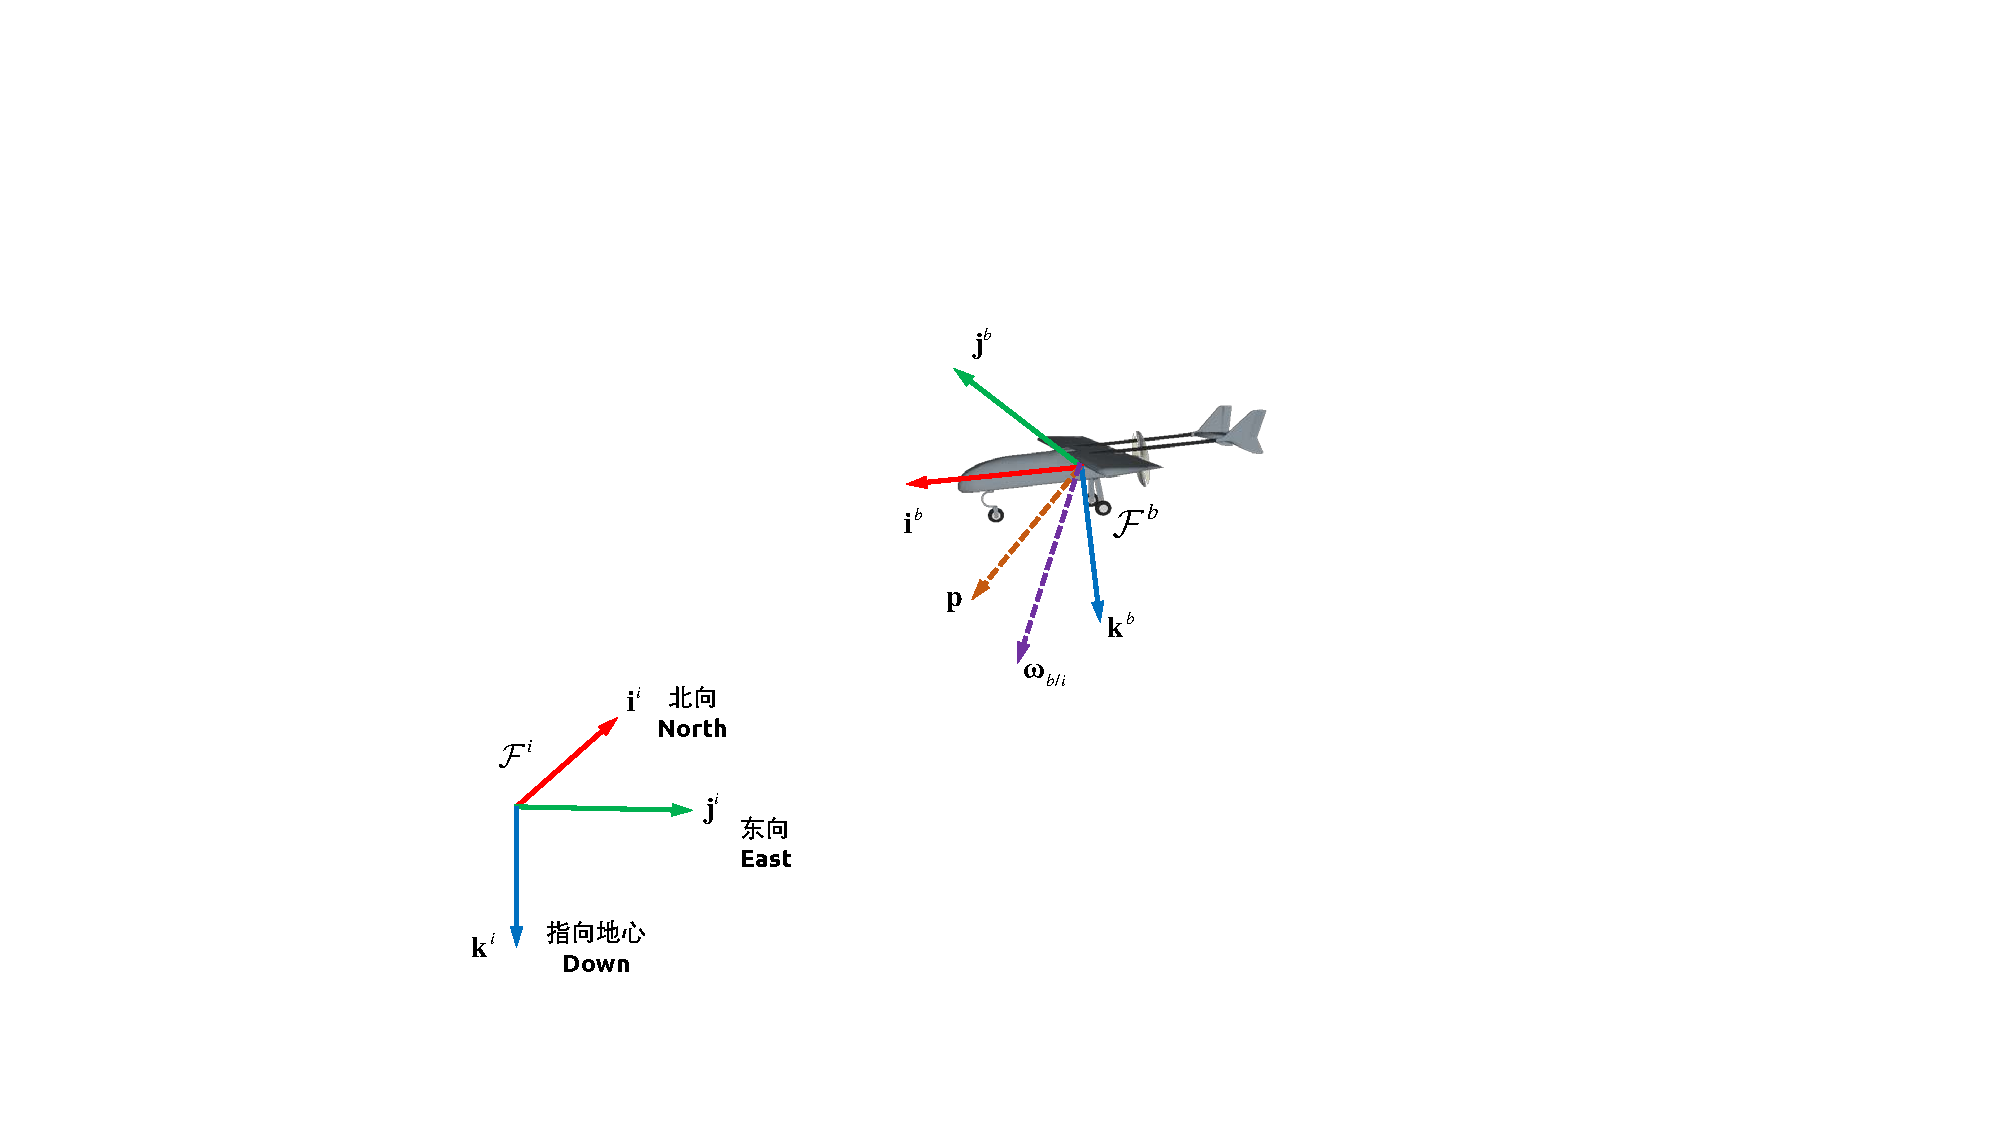
\includegraphics[width=0.8\textwidth]{figs/chp02/chp02_06_vector_rotation.pdf}
	\caption{三维空间向量微分}
	\label{fig:chp02_06_vector_rotation}
\end{figure}

此时机体坐标系$\mathcal{F}^b$与惯性坐标系$\mathcal{F}^i$只存绕转动向量$\mathbf{\omega}_{b/i}$的转动,不存在平动。由此得到该运动向量$\mathbf{p}$相对于系统坐标系$\mathcal{F}^i$的微分为
\begin{equation} \label{chp02_vector_derivative}
\frac{d}{dt_i} \mathbf{p} = \frac{d}{dt_b} \mathbf{p} + \mathbf{\omega}_{b/i} \times \mathbf{p}
\end{equation}
其中等式右侧的第一项具体表达为
\begin{equation}
\frac{d}{dt_i} \mathbf{p} = \dot{p}_x \mathbf{i}^b +  \dot{p}_y \mathbf{j}^b +  \dot{p}_z \mathbf{k}^b
\end{equation}
该部分可以通过设计无人机状态的观测器的获得。

\subsection{无人机空间位置定义}
因为飞机着舰过程的运动范围相对较小,由此对问题的坐标的整体构架主要选用Flat-Earth模型来替代WGS-84模型。首先,对于无人机在系统惯性系$\mathcal{F}^i$的位置定义为$(p_n\ p_e\ p_d)^T$,其中$n$, $e$  和$d$ 描述系统坐标系正北、正东和指向地心的方向。定义$h = -p_d$,用于描述无人机的飞行高度。无人机在系统惯性系的速度在机体坐标系$\mathcal{F}^b$的投影为$(u, v, w)$,无人机在机体坐标系$\mathcal{F}^b$的旋转角速度为$(p, q, r)$。则可以得到无人机速度在两个坐标系的相互转换关系
\begin{equation}
\frac{d}{dt} \begin{bmatrix} p_n \\ p_e \\ p_d \end{bmatrix}   =  (\mathcal{R}_v^b)^T \begin{bmatrix} u \\  v \\ w \end{bmatrix}  
\end{equation}
\begin{equation}
\resizebox{.9 \textwidth}{!} 
{ $
\begin{bmatrix} \dot{p}_n \\ \dot{p}_e \\ \dot{p}_d \end{bmatrix} = \begin{bmatrix}  cos \theta \cos \psi   &     -\cos\phi \sin\psi + \sin\phi \sin\theta \cos\psi                        &  \sin\phi \sin\psi + \cos\phi \sin\theta \cos\psi       \\
\cos\theta \sin\psi    & \cos\phi \cos\psi + \sin\phi \sin\theta\sin\psi   & -\sin\phi \cos\psi + \cos\phi \sin\theta \sin\psi \\
-\sin\theta  & \sin\phi \cos\theta & \cos\phi \cos\theta
\end{bmatrix} \begin{bmatrix} u \\  v \\ w \end{bmatrix}
$}
\end{equation}
进一步化解可以得到
\begin{align}
\begin{bmatrix} p \\ q \\ r \end{bmatrix}  &=   \begin{bmatrix}
1 &  0   & -\sin \theta      \\
0 &  \cos \phi  & \sin \phi \cos \theta \\	
0 & -\sin \phi   & \cos \phi \cos \theta
\end{bmatrix} \begin{bmatrix} \dot{\phi} \\ \dot{\theta} \\ \dot{\psi} \end{bmatrix} \\
\begin{bmatrix} \dot{\phi} \\ \dot{\theta} \\ \dot{\psi} \end{bmatrix}  &=  \begin{bmatrix}
1 &  \sin \phi \tan \theta  & - \cos \phi \tan \theta      \\
0 & \cos \phi   & -\sin \phi \\
0  & \sin \phi \sec \theta & \cos \phi \sec \theta
\end{bmatrix} \begin{bmatrix} p \\ q \\ r \end{bmatrix}
\end{align}

\subsection{无人机的外部力和力矩分析}
无人机的质量定义为$\mathsf{m}$,所受全部外力定义为$\mathbf{f}$,主要由重力$\mathbf{f}_g$、空气动力$\mathbf{f}_a$和电机拉力$\mathbf{f}_p$三部分组成
\begin{equation}
\mathbf{f} = \mathbf{f}_g + \mathbf{f}_a + \mathbf{f}_p
\end{equation}

重力在无人机惯性坐标系$\mathcal{F}^v$的表达为
\begin{equation}
\mathbf{f}_g^v = \begin{bmatrix}0  \\ 0  \\ \mathsf{m}g  \end{bmatrix}
\end{equation}

重力在无人机机体坐标系$\mathcal{F}^b$的表达为
\begin{equation}
\mathbf{f}_g^b =\mathcal{R}^b_v \begin{bmatrix}0  \\ 0  \\ \mathsf{m}g  \end{bmatrix} \\
= \begin{bmatrix} -\mathsf{m} g \sin \theta  \\ \mathsf{m}g \cos \theta \sin \phi  \\ \mathsf{m}g \cos\theta \cos \phi  \end{bmatrix}
\end{equation}

根据空气动力定义,在水平方向,无人机受到的升力$F_{lift}$、阻力$F_{drag}$和力矩$m$,其基本定义为
\begin{align}
F_{filt} = \frac{1}{2} V_a^2SC_L(\alpha, q, \delta_e) \\
F_{drag} = \frac{1}{2} V_a^2SC_D(\alpha, q, \delta_e) \\
m = \frac{1}{2} V_a^2ScC_m(\alpha, q, \delta_e)
\end{align}
其中$S$是机翼面积,$c$是机翼平均舷长,$C_L$、$C_D$和$C_m$是非线性空气动力参数。此外,无人机的控制面为三个,副翼偏移$\delta_a$,方向舵偏移$\delta_r$和升降舵偏移$\delta_e$。

根据本文目标无人机的空气特性,由此将上述气动力参数进一步展开为
\begin{align}
C_L(\alpha, q, \delta_e) &= C_X(\alpha) + {C_X}_q(\alpha) \frac{c}{2V_a}  q+ C_{X_{{\delta}_e}}(\alpha) \delta_e \\
C_D(\alpha, q, \delta_e) &= C_{Y_{0}} + C_{Y_{\beta}} \beta + C_{Y_r}(\alpha) \frac{b}{2V_a} r+ C_{Y_{\delta_\alpha}} \delta_\alpha +  C_{Y_{\delta_r}} \delta_r  \\ 
C_m(\alpha, q, \delta_e) &= C_Z(\alpha) + C_{Z_q}(\alpha) \frac{c}{2V_a}  q+ C_{Z_{\delta_e}} \delta_e
\end{align}
其中
\begin{align}
C_X(\alpha) &= -C_D(\alpha) \cos \alpha +  C_L(\alpha) \sin \alpha \\
C_{X_q}(\alpha) &= -C_{D_q} \cos \alpha +  C_{L_q} \sin \alpha \\
C_{X_{\delta_e}}(\alpha) &= -C_{D_{\delta_e}} \cos \alpha +  C_{L_{\delta_e}} \sin \alpha \\
C_Z(\alpha) &= -C_D(\alpha) \cos \alpha -  C_L(\alpha) \sin \alpha \\
C_X(\alpha) &= -C_{D_q} \sin \alpha -  C_{L_q} \cos \alpha \\
C_X(\alpha) &= -C_{D_{\delta_e}}  \sin \alpha -  C_{L_{\delta_e}} \cos \alpha \\
\end{align}
因为升力和阻力作用在无人机稳定坐标系$\mathcal{F}^s$上,因此将上述力转换到无人机的机体坐标系后,进一步得到
\begin{align}
\begin{bmatrix} f_x    \\ f_z  \end{bmatrix} = \begin{bmatrix}
\cos \alpha    & - \sin \alpha  \\
\sin \alpha       & \cos \alpha  \\
\end{bmatrix} \begin{bmatrix} -F_{drag}    \\ -F_{lift}  \end{bmatrix}
\end{align}
在竖直方向,无人机受到竖直方向的力和力矩为
\begin{align}
f_y = \frac{1}{2} \rho V_a^2 S C_y (\beta, p, r, \delta_a, \delta_r) \\
l  = \frac{1}{2} \rho V_a^2 S b  C_l (\beta, p, r, \delta_a, \delta_r) \\
n = \frac{1}{2} \rho V_a^2 S b C_n (\beta, p, r, \delta_a, \delta_r)
\end{align}
其中,$C_y$、$C_l$和$C_n$是非线性空气动力参数。

螺旋桨的推力建模为
\begin{equation}
\mathbf{f}_p = \frac{1}{2} \rho S_{prop} C_{prop}  \begin{bmatrix} (\mathsf{k}_{motor} \delta_t)^2 - V_a^2  \\ 0  \\ 0  \end{bmatrix}
\end{equation}
其中$\mathsf{k}_{motor}$是电机效率常数,$\delta_t$是电机的控制量,$S_{prop}$是螺旋桨的面积,$C_{prop}$是螺旋桨参数。

螺旋桨的力矩建模为
\begin{equation}
\mathbf{T}_p = -\mathsf{k}_{T_p} (\mathsf{k}_{\Omega} \delta_{t})^2
\end{equation}

其中$\Omega = \mathsf{k}_{\Omega} \delta_{t}$是螺旋桨的转速,$\mathsf{k}_{T_p}$是电机常数。

\subsection{无人机的平动分析}
对于无人机的平动,无人机的质量为$\mathsf{m}$和其受到的全部外力$\mathbf{f}$,根据顿第二定律可以得到
\begin{equation}
\mathsf{m} \frac{d \mathbf{V}_g}{d t_i} = \mathbf{f}
\end{equation}
代入\ref{chp02_vector_derivative}公式,可以得到
\begin{equation}
\mathsf{m}(\frac{d \mathbf{V}_g }{dt_b}+ \mathbf{\omega}_{b/i} \times \mathbf{V}_g)=\mathbf{f}
\end{equation}
同理,在机体坐标系$\mathcal{F}^b$可以得到
\begin{equation}
\mathsf{m}(\frac{d \mathbf{V}^b_g }{dt_b}+ \mathbf{\omega}_{b/i}^b \times \mathbf{V}^b_g)=\mathbf{f}^b
\end{equation}
其中$\mathbf{V}_g^b=(u, v, w)^T$描述无人机惯性系的速度向量在机体坐标系的表达,$\frac{d \mathbf{V}_g }{dt_b}=(\dot{u}, \dot{v}, \dot{w})^T$描述无人机速度在机体坐标系的变化率,$\mathbf{\omega}_{b/i}^b=(p, q, r)^T$描述无人机机体坐标系的转动角速度,$\mathbf{f}^b = (f_x, f_y, f_z)^T$描述外部合力向量在机体坐标系的表达。进一步可以得到
\begin{equation}
\begin{bmatrix} \dot{u} \\ \dot{v} \\ \dot{w}  \end{bmatrix} = \begin{bmatrix} rv-qw \\ pw-ru \\ qu-pv  \end{bmatrix} + \frac{1}{\mathsf{m}} \begin{bmatrix} f_x \\ f_y \\ f_z  \end{bmatrix}
\end{equation}



\subsection{无人机的转动分析}
对于无人机对转动,定义角动量$\mathbf{h}$和全部外力矩$\mathbf{m}$,由此可以得到
\begin{equation}
\frac{ d \mathbf{h}}{d t_i}=\mathbf{m}
\end{equation}
同理,对上式求在惯性系的微分
\begin{equation}
\frac{ d \mathbf{h}}{d t_i} = \frac{d\mathbf{h}}{dt_b} + \mathbf{\omega}_{b/i} \times \mathbf{h} = \mathbf{m}
\end{equation}
同理,在机体坐标系的表达为
\begin{equation}
\frac{ d \mathbf{h}^b}{d t_i} = \frac{d\mathbf{h}^b}{dt_b} + \mathbf{\omega}^b_{b/i} \times \mathbf{h}^b = \mathbf{m}^b
\end{equation}
对于刚体来说,角动量的表达通过惯量矩阵$\mathbf{J}$来定义
\begin{equation}
\mathbf{h}^b=\mathbf{J}  \mathbf{\omega}^b_{b/i}
\end{equation}
其中
\begin{align}
\mathbf{J} =\begin{bmatrix}	\int(y^2 + z^2)~d\mathsf{m} & -\int xy \ d\mathsf{m}        & -\int xz~d\mathsf{m} \\	-\int xy~d\mathsf{m}        & \int(x^2 + z^2)~d\mathsf{m} & -\int yz~d\mathsf{m} \\	-\int xz~d\mathsf{m}        & -\int yz~d\mathsf{m}  & \int(x^2 + y^2)~d\mathsf{m} \end{bmatrix}
\end{align}
根据无人机机体的对称性,该矩阵可以化简为
\begin{align}
\mathbf{J} = \begin{bmatrix}	J_x     & 0   & -J_{xz} \\	0       & J_y & 0       \\	-J_{xz} & 0   & J_z  \end{bmatrix}
\end{align}
改矩阵的逆为
\begin{align}
\mathbf{J}^{-1}=\frac{\mathrm{adj}(\mathbf{J}) }{\mathrm{det}(\mathbf{J}) } = \begin{bmatrix}	J_z / \Gamma     & 0   & J_{xz}/ \Gamma \\	0       & 1/ \Gamma & 0       \\	J_{xz}/ \Gamma & 0   & J_z/ \Gamma \end{bmatrix}
\end{align}
其中$ \Gamma = J_xJ_z - J_{xz}^2$ 。

同时,定义上式中的分量
\begin{align}
\dot{\mathbf{\omega}}^b_{b/i}=\frac{ d \mathbf{\omega}^b_{b/i}}{dt_b} = \begin{bmatrix} \dot{p} \\ \dot{q} \\ \dot{r}  \end{bmatrix}
\end{align}
该分量描述在机体坐标系角速度的变化率。

根据上述公式可以得到对角速度变化率的求解
\begin{equation}
\dot{\mathbf{\omega}}^b_{b/i} = \mathbf{J}^{-1}[{- \mathbf{\omega}}^b_{b/i} \times (\mathbf{J{\mathbf{\omega}}^b_{b/i}})+\mathbf{m}^b]
\end{equation}
定义无人机力矩在机体坐标系的表达$\mathbf{m}^b = (l, m, n)$

则可以得到对角速度变化率的进一步表达
\begin{equation}
\begin{bmatrix} \dot{p} \\ \dot{q} \\ \dot{r}  \end{bmatrix} =  \begin{bmatrix} \Gamma_1pq - \Gamma_2qr + \Gamma_3 l + \Gamma_4 n \\ \Gamma_5pr - \Gamma_6(p^2-r^2) + \frac{1}{Jy}m \\ \Gamma_7pq - \Gamma_1qr + \Gamma_4l + \Gamma_8 n  \end{bmatrix}
\end{equation}
其中各个分量的表达为
\begin{align}
\Gamma_1 &= \frac{J_{xz}(J_x-J_y+J_z)}{\Gamma}  \\
\Gamma_2 &= \frac{J_z(J_z-J_y) + J_{xz}^2}{\Gamma}  \\
\Gamma_3 &= \frac{J_z}{\Gamma}  \\
\Gamma_4 &= \frac{J_{xz}}{\Gamma}  \\
\Gamma_5 &= \frac{J_z - J_x}{J_y}  \\
\Gamma_6 &= \frac{J_{xz}}{J_y}  \\
\Gamma_7 &= \frac{(J_x-J_z)J_x+J_{xz}^2}{\Gamma}  \\
\Gamma_8 &= \frac{J_x}{\Gamma}  \\
\end{align}
 
\subsection{无人机运动轨迹数学描述}

\begin{figure}[htb]   
	\centering
	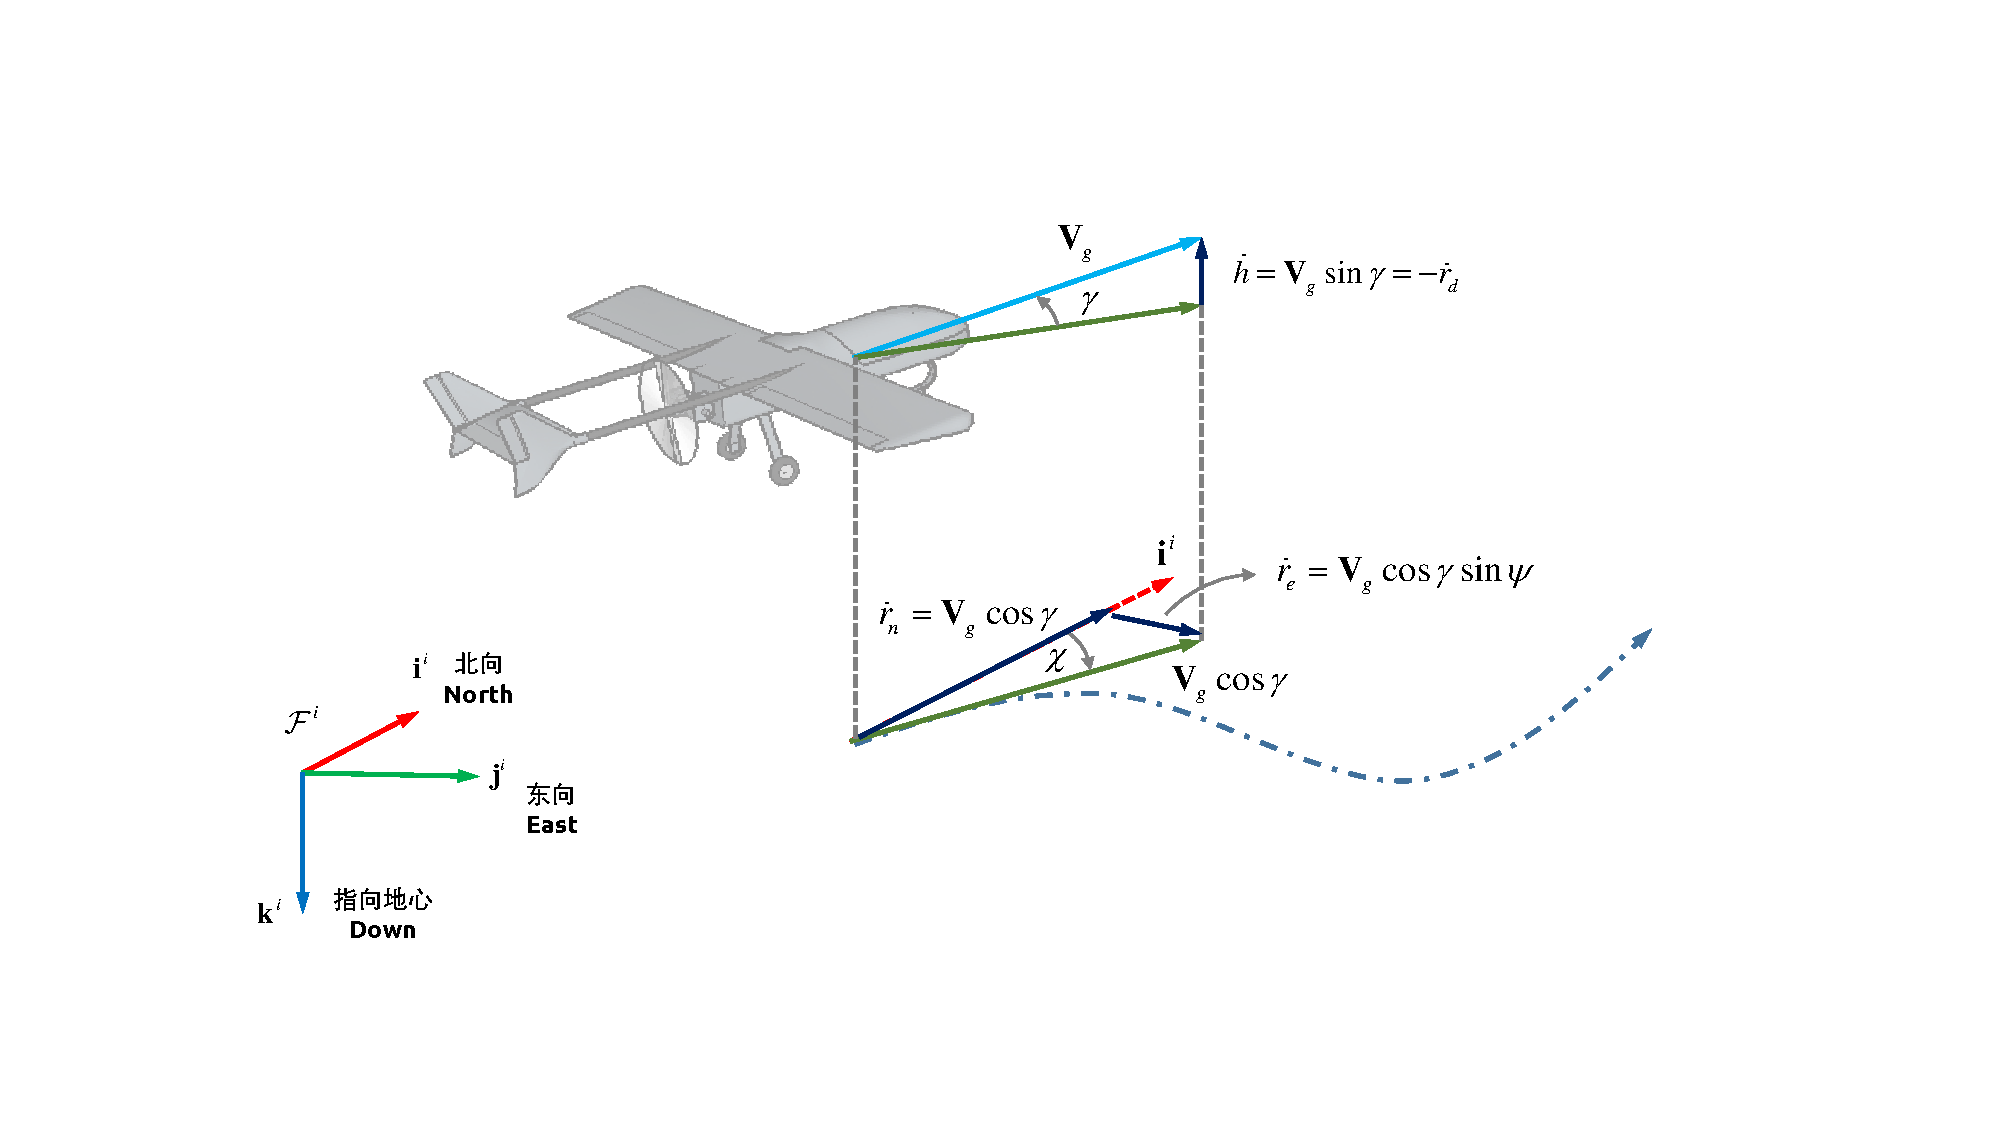
\includegraphics[width=0.8\textwidth]{figs/chp02/chp02_05_uav_course_frame.pdf}
	\caption{无人机运动轨迹描述}
	\label{fig:chp02_05_uav_course_frame}
\end{figure}

定义无人机在惯性系的坐标为$(p_n\ p_e\ p_d)^T$,无人机速度$\mathbf{V}_g$在惯性系的分量为$(\dot{p}_n\ \dot{p}_e\ \dot{p}_d)^T$,该速度的大小用$V_g = ||\mathbf{V}_g||$来表达,如图\ref{fig:chp02_05_uav_course_frame}所示。根据空间几何关系可以得到
\begin{equation}
\begin{bmatrix} \dot{p}_n \\\dot{p}_e \\ \dot{p}_d \end{bmatrix}  = {V}_g \begin{bmatrix} \cos \psi \cos \gamma \\ \sin \psi \cos \gamma  \\- \sin \gamma \end{bmatrix}
\end{equation}
其中航迹角$\gamma$定义为地速$\mathbf{V}_g$与惯性系北向$\mathbf{i}^i$与动向$\mathbf{j}^i$所构成的地平面的夹角,航迹偏航角$\chi$定义为地速$\mathbf{V}_g$在地面投影与正北方向的夹角。

由于无人机受到的升力为$F_{lift}$,在无人机进行协同转向(Coordinated Turn)时,根据力学关系可以得到横向和纵向公式
\begin{align}
&F_{lift} \sin \phi \cos (\chi - \psi) = \mathsf{m} \frac{v^2}{R}  \\
&F_{lift } \cos \phi = \mathsf{m} g \cos \gamma
\end{align}
将上述两式相除,并对$\chi$微分,可以得到
\begin{equation}
\dot{\chi} = \frac{g}{V_g} \tan \phi \cos (\chi - \psi)
\end{equation}
在没有风速影响下($V_g = V_a\ , \psi = \chi$),可以将上式进一步化简为
\begin{equation}
\dot{\psi} =\frac{g}{V_a} \tan \phi
\end{equation}
因为无人机的控制一般分为内环和外环,内环的控制速率较快,即飞行控制器可以很快使得无人机的姿态角收敛到指令期望位置,即$\gamma = \gamma^c\ , \phi = \phi^c$。因此,无人机的运动情况可以通过如下公式进一步描述
\begin{equation}
\begin{bmatrix} \dot{p}_n \\\dot{p}_e \\ \dot{p}_d \end{bmatrix}  = {V}_a \begin{bmatrix} \cos \psi \cos \gamma^c \\ \sin \psi \cos \gamma^c  \\- \sin \gamma^c \end{bmatrix} \\
\dot{\psi} =\frac{g}{V_a} \tan \phi^c
\end{equation}
由于无人机执行机构的物理约束,无人机的控制指令收到进一步约束
\begin{align}
|\phi^c| \le \bar{\phi} \\
|\gamma^c| \le \bar{\gamma}
\end{align}
其中$\bar{\phi}$和$\bar{\gamma}$为无人机系统的最大横滚角和下滑角约束。


\section{舰船系统坐标系定义}

舰船坐标系主要由舰船惯性坐标系、舰船龙骨坐标系和着舰点坐标系三部分组成。
\subsection{舰船惯性坐标系}
舰船惯性坐标系($\mathcal{F}^{Sh,i}$,Ship Inertial Frame),该坐标系的原点定义在舰船的中心位置,一般位于龙骨所在轴线,位于甲板下方。该坐标系的三个轴的方向分别与系统坐标系$\mathcal{F}^i$平行。该坐标系的表达如图\ref{fig:chp02_08_ship_interial_frame}所示。

\begin{figure}[htb]   
	\centering
	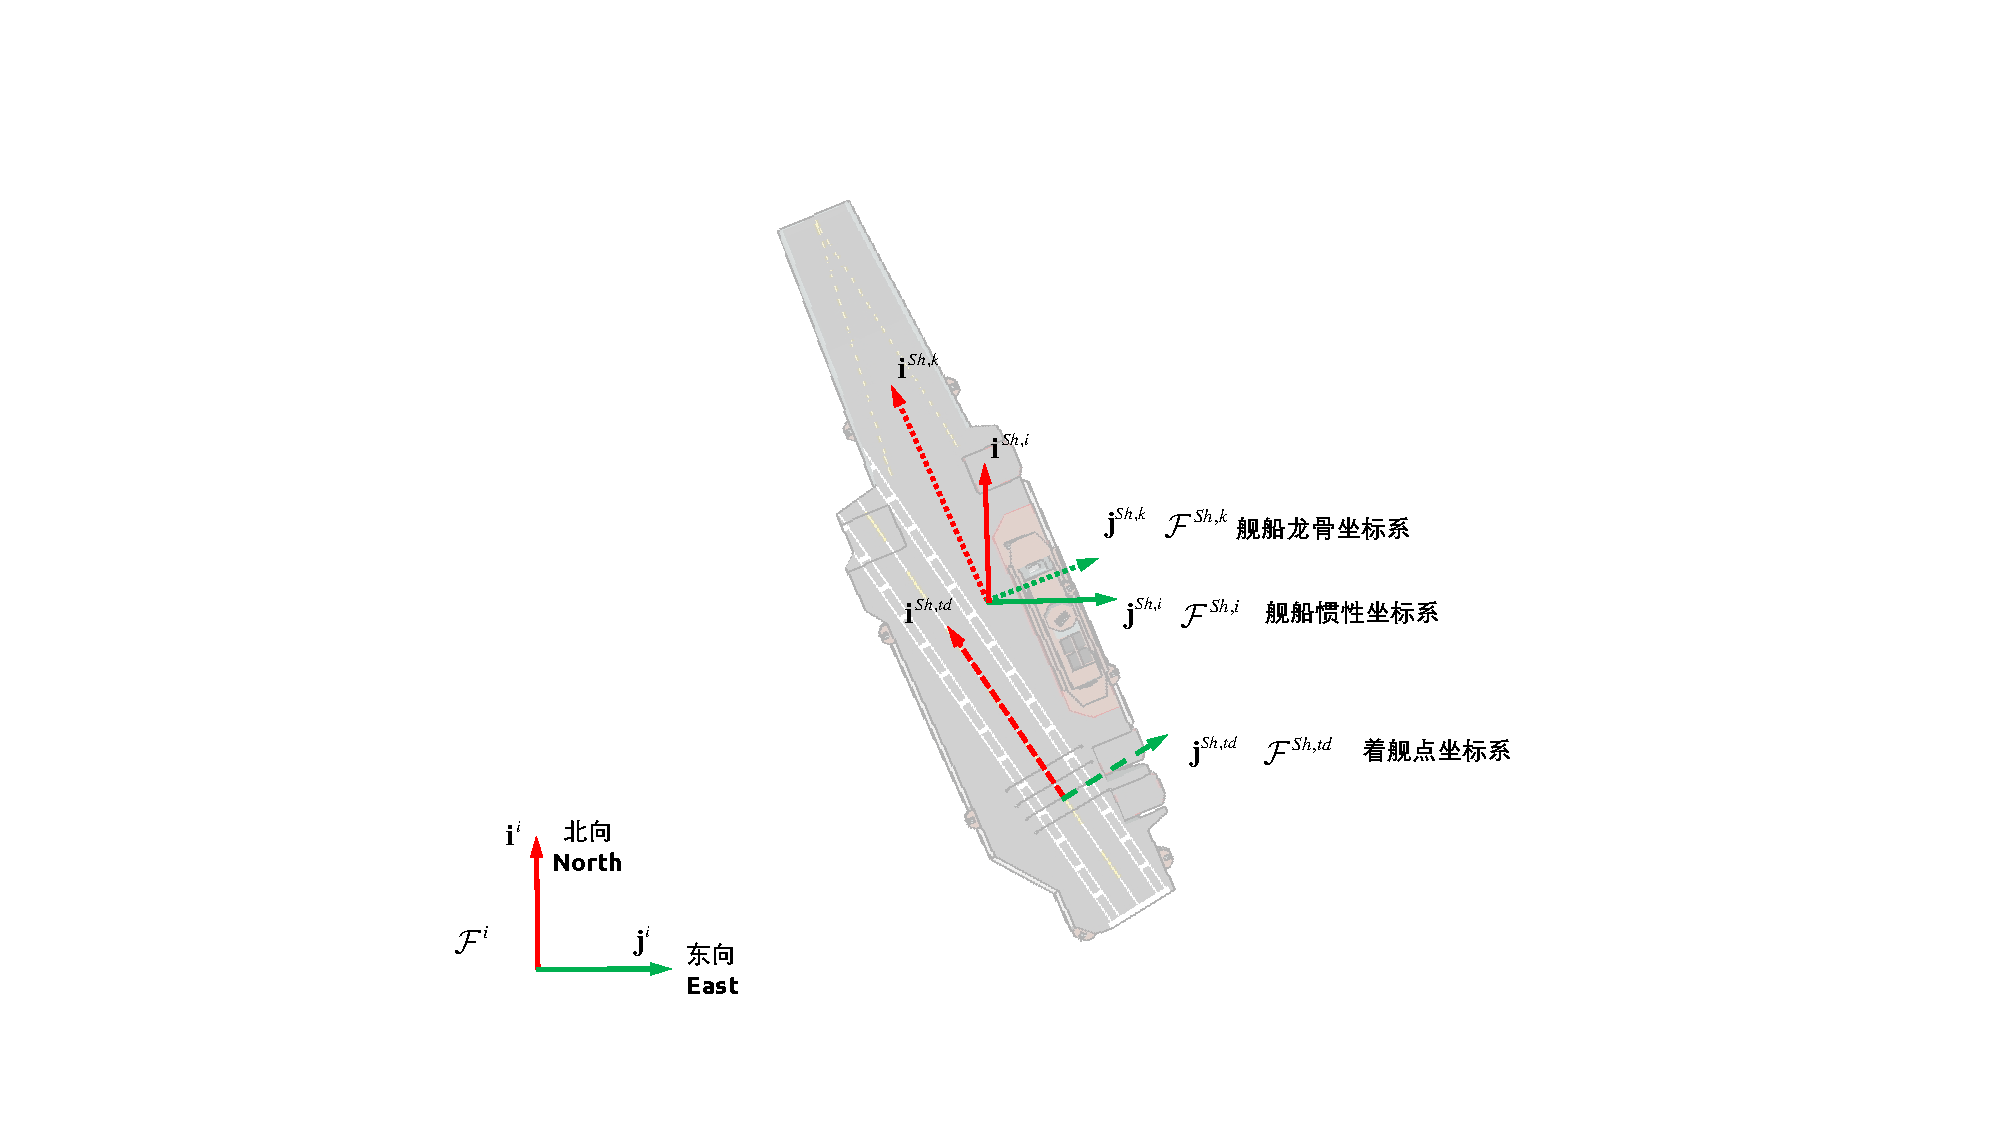
\includegraphics[width=0.8\textwidth]{figs/chp02/chp02_08_ship_interial_frame.pdf}
	\caption{舰船惯性坐标系}
	\label{fig:chp02_08_ship_interial_frame}
\end{figure}

\subsection{舰船龙骨坐标系}
舰船龙骨坐标系($\mathcal{F}^{Sh,k}$ ,Keel Frame),该坐标系的原点与舰船惯性坐标系相同,$\mathbf{i}^{Sh,k}$轴沿龙骨方向指向舰船前进方向,$\mathbf{j}^{Sh,k}$轴垂直于$\mathbf{i}^{Sh,k}$方向。因为该坐标系与船体固连,所以海浪的作用下,该坐标系随船体运动。与无人机机体坐标系类似,将舰船惯性坐标系按照3-2-1的顺序依次旋转至舰船龙骨坐标系,定义三次转动的角度为$\phi_{Sh}$、$\theta_{Sh}$和$\psi_{Sh}$,用于描述舰船的俯仰角、横滚角和偏航角。不同海况情况下,舰船龙骨坐标系还会存在周期性的扰动,由此定义$\Delta \phi_{Sh}$、$\Delta \theta_{Sh}$和$\Delta \psi_{Sh}$来描述舰船龙骨坐标系在俯仰、横滚和偏航三个轴线的扰动角度,定义$\Delta x_{surge}$、$\Delta y_{sway}$和$\Delta z_{heavy}$来描述三个坐标轴的位移偏差,即横摇、纵摇和沉浮。该坐标系的表达如图\ref{fig:chp02_09_ship_motion_frame}所示。

\begin{figure}[htb]   
	\centering
	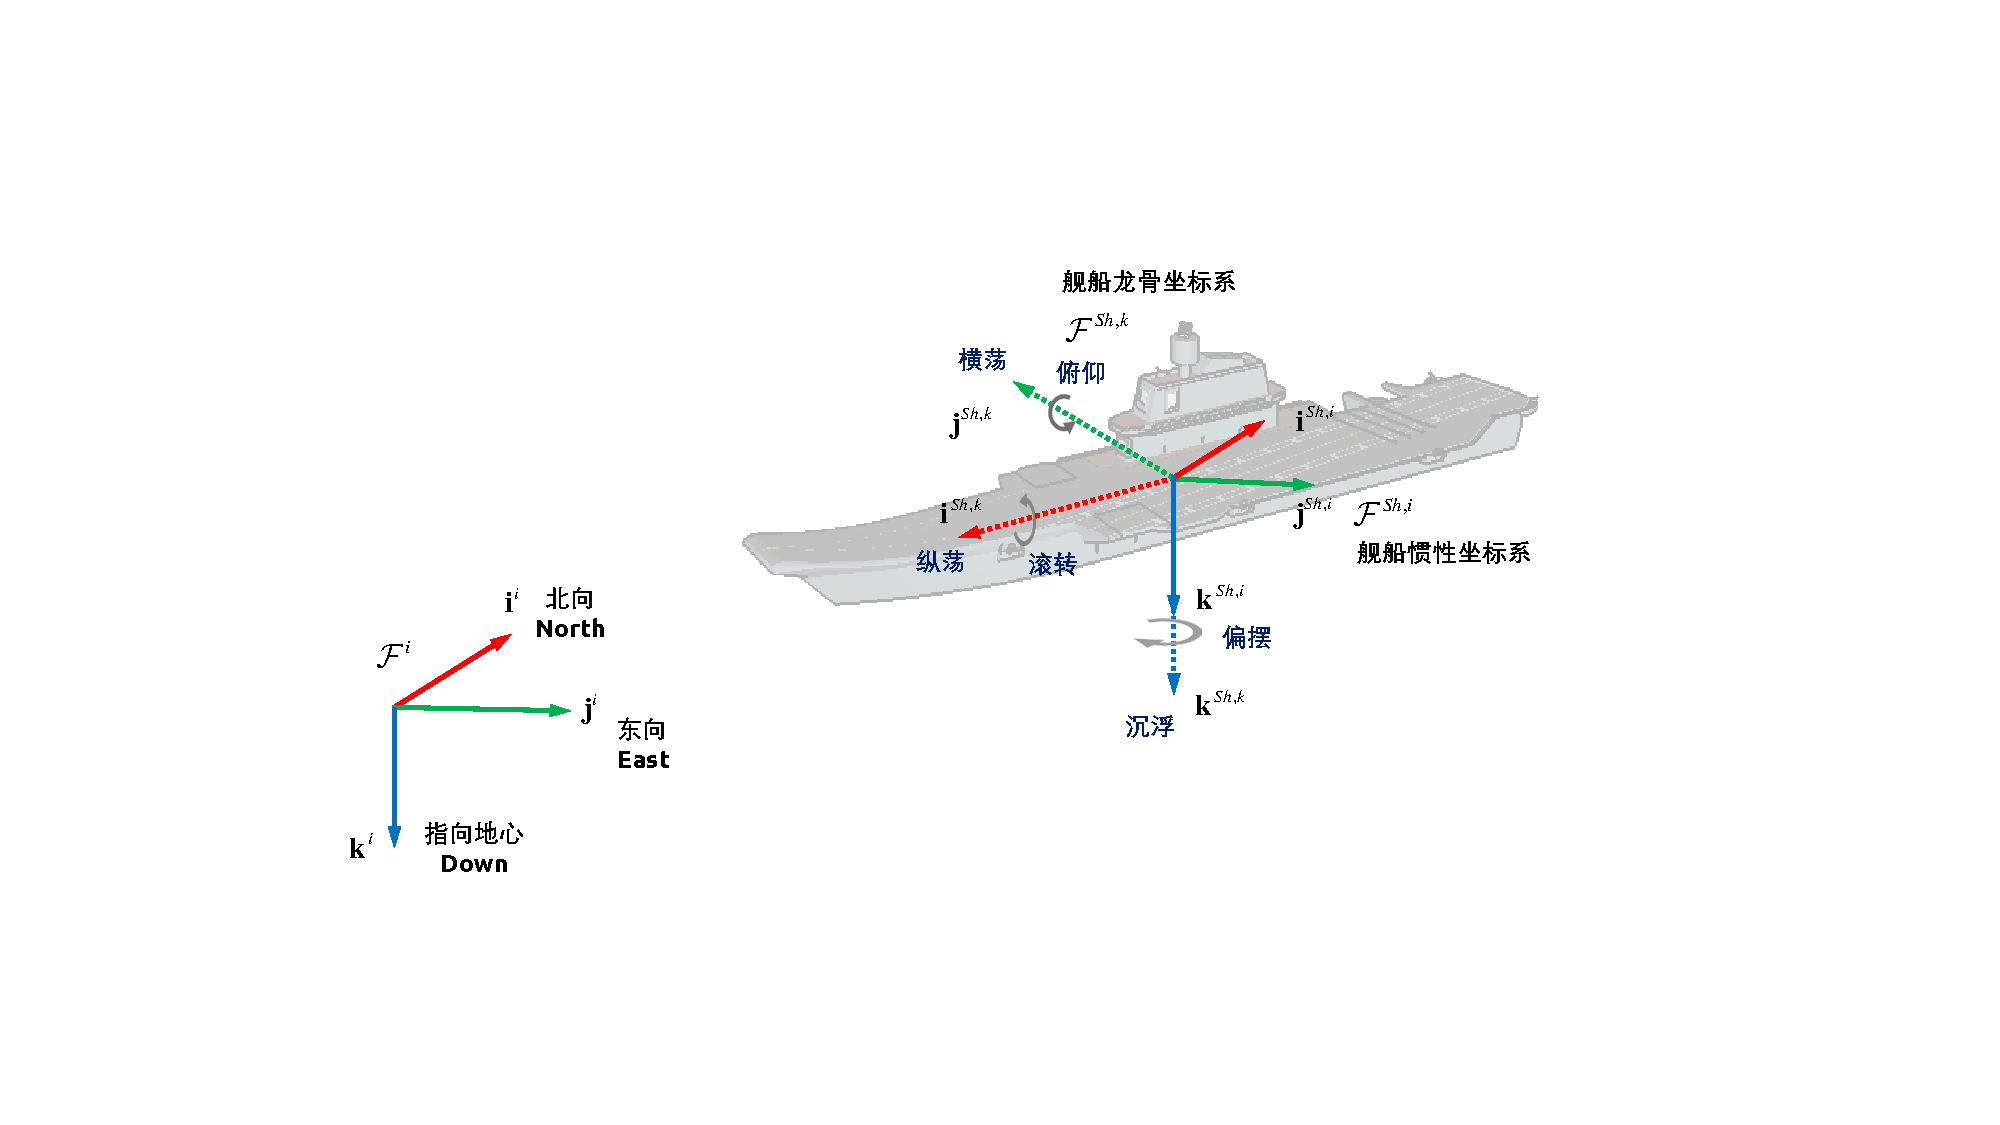
\includegraphics[width=\textwidth]{figs/chp02/chp02_09_ship_motion_frame.pdf}
	\caption{舰船系统坐标系的表达}
	\label{fig:chp02_09_ship_motion_frame}
\end{figure}


\subsection{着舰点坐标系}
着舰点坐标系($\mathcal{F}^{Sh,td}$,Touchdown Frame),该坐标系原点定义在第二条拦阻索的中间位置,$\mathbf{i}^{Sh,td}$轴沿降落跑道指向舰船运行前方,$\mathbf{j}^{Sh,td}$轴沿第二条拦阻索方向延长垂直于$\mathbf{i}^{Sh,td}$轴。

着舰点坐标系与舰船龙骨坐标系之间的转换关系定义为
\begin{equation}
\begin{bmatrix} x_{Sh,td} \\ y_{Sh,td} \\z_{Sh,td} \end{bmatrix} = \begin{bmatrix} x_{Sh,k} \\ y_{Sh,k} \\z_{Sh,k} \end{bmatrix} +\mathcal{R}_{Sh,k}^{Sh,td} \begin{bmatrix} \Delta x_{Sh,k}^{Sh,td} \\ \Delta y_{Sh,k}^{Sh,td} \\ \Delta z_{Sh,k}^{Sh,td} 
\end{bmatrix}
\end{equation}
其中$\Delta x_{Sh,k}^{Sh,td}$,$\Delta y_{Sh,k}^{Sh,td}$和$\Delta z_{Sh,k}^{Sh,td}$是着舰坐标系原点在舰船龙骨坐标系的坐标,$\mathcal{R}_{Sh,k}^{Sh,td}$是从舰船坐标系旋转到着舰点坐标系的旋转矩阵,该旋转矩阵的表达形式与无人机机体惯性坐标系转换到无人机机体坐标系的旋转矩阵相同,$(x_{Sh,k}\ y_{Sh,k}\ z_{Sh,k})$是舰船惯性坐标系上一点,该点在舰船着舰点坐标系上的坐标为$(x_{Sh,td}\ y_{Sh,td}\ z_{Sh,td})$。

\section{舰载引导系统坐标系定义}
由于舰船的运动,对于降落过程中的无人机需要提供有效的局部导航数据,本文设计的舰载引导系统坐标系主要用于描述引导系统对无人机的测量和导航。
\subsection{引导系统坐标系}
引导系统坐标系(Guidance Coordination System, $\mathcal{O}_c$)该坐标系的原点位于左侧引导系统的转台转轴的中心,$\mathbf{i}^{O,c}$轴指向右侧引导系统,并与着舰点坐标系的$\mathbf{j}^{Sh,td}$轴平行,$\mathbf{j}^{O,c}$轴与跑道纵向平行,指向远端无人机方向。该坐标系在舰船运动过程中与甲板固连,与期望着舰点坐标系的位置保持不变。一般而言,对于无人机着舰而言,期望着舰点的位置位于第一道和第二道拦阻索之间,靠近第二道拦阻索,如图\ref{fig:chp02_10_guidance_sys}所示;对于无人机装网回收而言,期望降落位置一般位于无人机回收网的几何中心。
\begin{figure}[htb]   
	\centering
	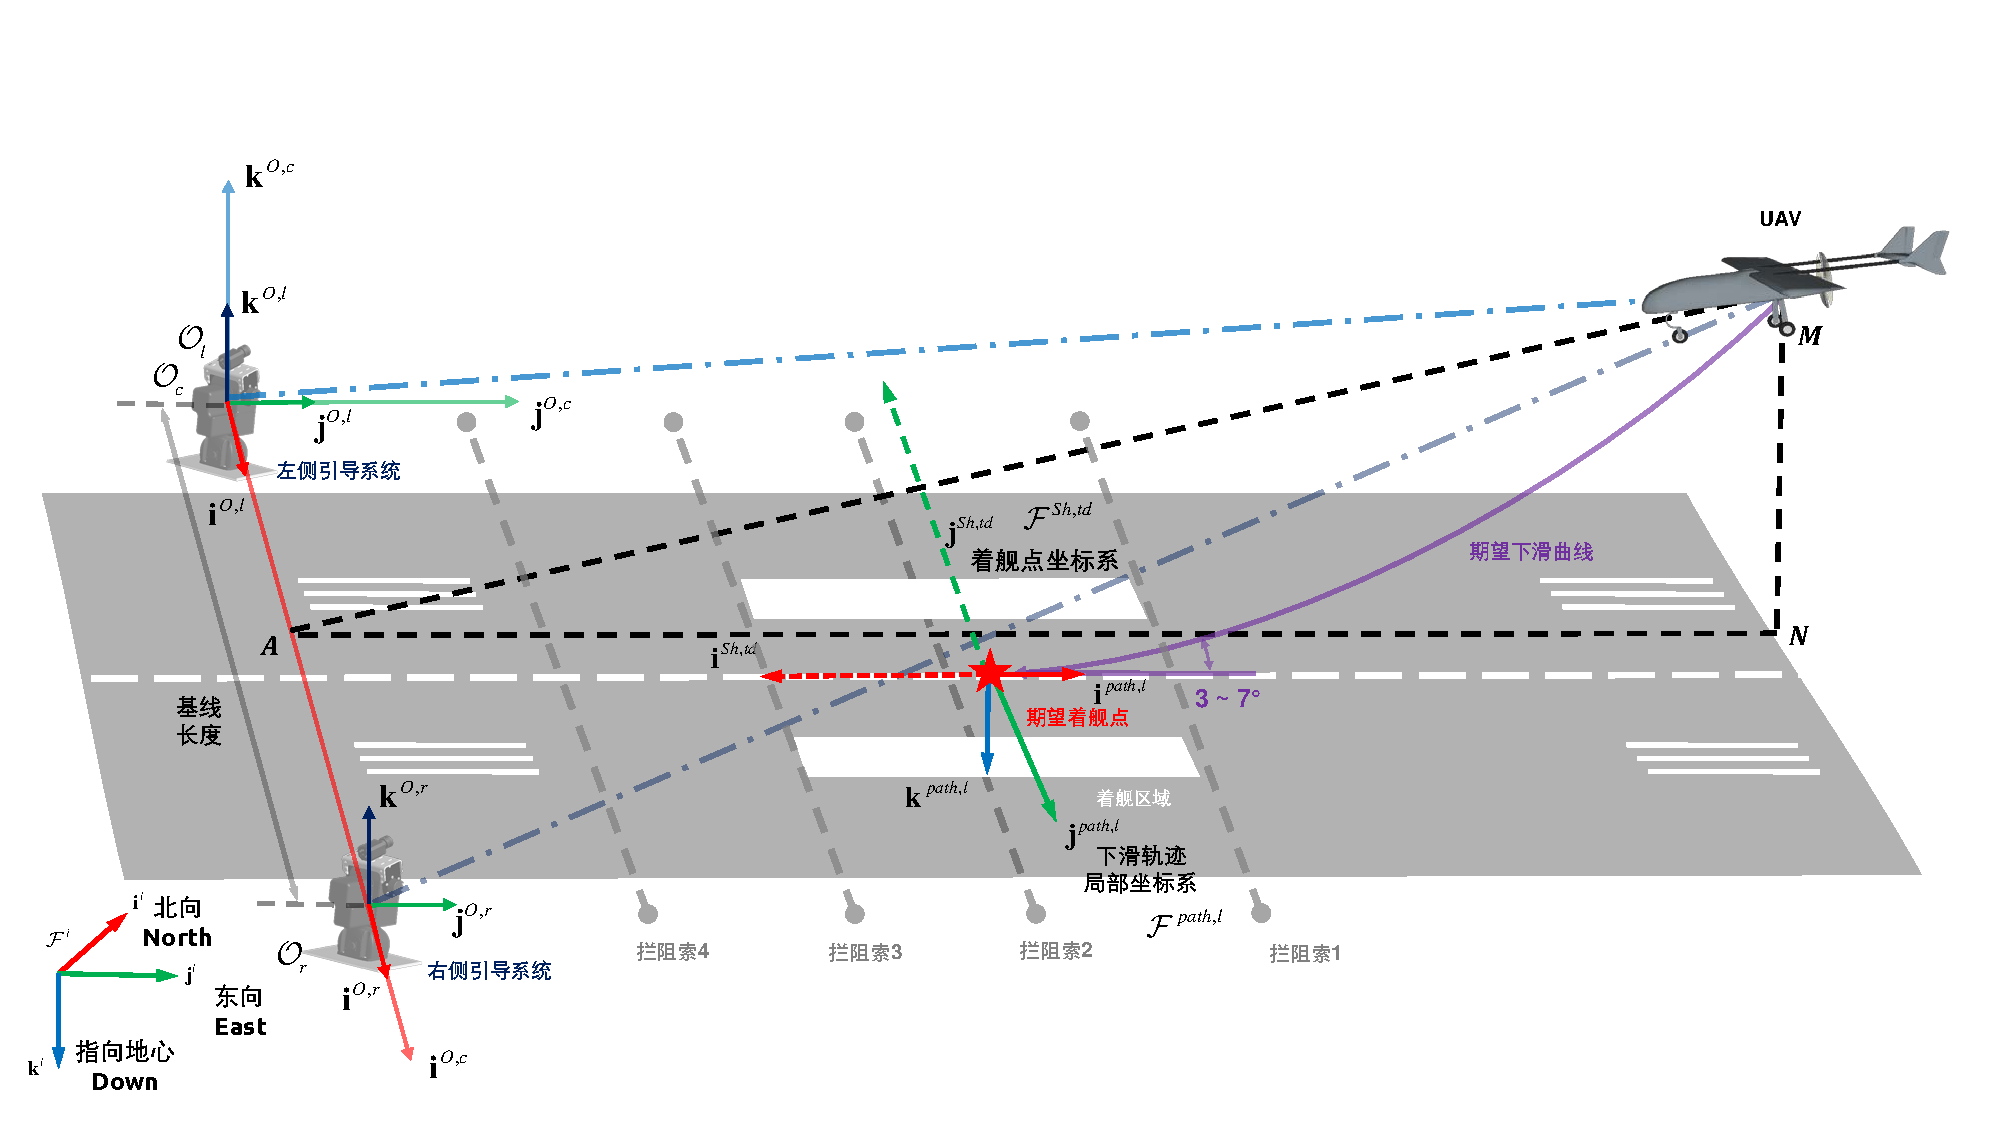
\includegraphics[width=\textwidth]{figs/chp02/chp02_10_guidance_sys.pdf}
	\caption{舰载引导系统相关坐标系}
	\label{fig:chp02_10_guidance_sys}
\end{figure}

\subsection{左右引导单元坐标系}
左侧引导系统坐标系($\mathcal{O}_l$)和右侧引导系统坐标系($\mathcal{O}_r$),这两个坐标系的原点别位于左侧和右侧引导系统的转台转轴中心,三个坐标轴的方向分别与光学引导系统相同。该引导单元坐标系也是用于立体解算无人机空间位置的主要坐标系。

\subsection{地心地固坐标系}
地心地固坐标系(Earth-Centered Earth-Fixed Coordinate System (ECEF),$\mathcal{O}_e$),该坐标系采用1984年\cite{WGS84}指定的地心空间右手坐标系(The World Geodetic System (WGS-84)),原点位于地球中心,$x$轴指向地球0°经线和0°纬线的交叉点,$y$轴指向地球的北极点。该坐标系通常用于大地测量、地图绘制和导航。本文后续试验中使用的该坐标系相关参数为 $R_{Ea}=6,378,137.0\ m$,$R_{Eb} = 6,356,752.0\ m$ ,$f=1/298.257223563$ 和 $e=0.08181919$。

\subsection{GPS坐标系}
GPS坐标系(The Geodetic Coordination System,$\mathcal{O}_g$)中的任意一点通常用$(\lambda\ \varphi\ h)$表示,其中 $\lambda$ 表示目标当前位置的经度, $\varphi$ 表示目标当前位置的纬度, $h$ 表示当前位置的高度。该数值一般通过GPS解算模块获得。

\subsection{GPS坐标系与地心地固坐标系之间的转换关系}
定义GPS经纬坐标系中任意一点$\mathbf{P}^g=(\lambda, \varphi, h)$,该点在地心地固坐标系的表达为

\begin{equation}
\textbf{P}^e
=
\left[\begin{array}{c}
X_e\\
Y_e\\
Z_e\\
\end{array}\right]
=
\left[\begin{array}{c}
(N_E+h)\cos \varphi \cos \lambda\\
(N_E+h)\cos \varphi \sin \lambda\\
(N_E(1-e^2)+h)\sin \varphi\\
\end{array}\right]
\end{equation}

其中$N_E$是基于当前纬度位置的参数,根据上文所述的相关参数,该数值通常通过下式进行计算。

\begin{equation}
N_E=\frac{R_{Ea}}{\sqrt{1-e^2 \sin^2 \varphi}}.
\end{equation}

\subsection{地心地固坐标系与系统惯性坐标系之间的转换关系}
定义系统惯性系原点在地心地固坐标系的原点为$\mathbf{P}_0^e(x_0\ y_0\ z_0)$,该点的GPS经纬坐标为$\mathbf{P}_0^g(\lambda_0\ \varphi_0\ h_0)$,地心坐标系中任意一点$\mathbf{P}^e$在系统惯性坐标系的表达为

\begin{equation}
\textbf{P}^i=\mathcal{R}_e^n(\textbf{P}^e - \textbf{P}_0^e)
\end{equation}

其中转换矩阵$\mathcal{R}_e^n$为

\begin{equation}
\mathcal{R}_e^n=\left[\begin{array}{ccc}
-\sin \varphi _{0} \cos \lambda _{0} & -\sin \varphi _{0} \sin \lambda _{0} & \cos \varphi _{0}  \\
-\sin \lambda _{0}           &           \cos \lambda _{0}            &          0           \\
-\cos \varphi _{0} \cos \lambda _{0} & -\cos \varphi _{0} \sin \lambda _{0} & -\sin \varphi _{0}
\end{array}\right]
\end{equation}

\subsection{舰船惯性坐标系与引导坐标系之间的转换关系}
定义在舰船惯性坐标系中的一点为$\mathbf{P}^{Sh,i}(X_{Sh,i}\ Y_{Sh,i}\ Z_{Sh,i})$,该点对应在引导坐标系的坐标为$\mathbf{P}^{c}(X_c\ Y_c\ Z_c)$,这两点之间的转换关系可以通过平移和旋转运算$(X_{Sh,i}, Y_{Sh,i}, Z_{Sh,i})\xrightarrow{\textbf{R}_{Sh,i}^c,T}(X_c, Y_c, Z_c) $得到,其矩阵表达形式为

\begin{equation}
\left[\begin{array}{c}
X_{Sh,i}\\
Y_{Sh,i}\\
Z_{Sh,i}\\
\end{array}\right]=\mathcal{R}_{Sh,i}^c
\left[\begin{array}{c}
X_{c}\\
Y_{c}\\
Z_{c}\\
\end{array}\right]+T_{Sh,i}^c
\end{equation}
其中
\begin{equation}
\mathcal{R}_{Sh,i}^c=\left[\begin{array}{ccc}
r_{11} & r_{12} & r_{13} \\
r_{21} & r_{22} & r_{23} \\
r_{31} & r_{32} & r_{33} 
\end{array}\right]
\ \ 
T_{Sh,i}^c=\left[\begin{array}{ccc}
t_{Sh,i}^c\\
t_{Sh,i}^c\\
t_{Sh,i}^c\\
\end{array}\right]
\end{equation}
理想情况下,舰船惯性坐标系与引导坐标系之间的几何关系可以通过定义旋转和平移量获得,但由于引导系统的安装误差,该矩阵通常通过外部标定方法得到。


​





	%\chapter{舰基无人机立体视觉引导系统}
\section{引言}
由于视觉传感器具有成本较低和感知信息量较大的特性,该类型传感器被广泛应用于无人机引导与控制领域。本章通过误差分析和理论推导,设计基于立体视觉成像的短基线和长基线引导系统,实现对无人机相对位置的测量。

\section{短基线无人机视觉引导系统}
\subsection{相机成像模型}
本文使用的相机模型为小孔成像模型(Pin-hole Camera Model)。已知目标点$M$的三维空间坐标为$(x,y,z)$,则该坐标与像平面坐标$(u,v)$以及相机焦距$f$之间的关系用其次坐标的形式表达为
\begin{equation}
\lambda\left[ {\begin{array}{*{20}{c}}
	u \\ 
	v \\ 
	f 
	\end{array}} \right] =\left[ {\begin{array}{*{20}{c}}
	x \\ 
	y \\ 
	z 
	\end{array}} \right]
\end{equation}
其中$\lambda$是尺度因子。如果转换为欧拉坐标系,则可以得到
\begin{equation}
\left[ {\begin{array}{*{20}{c}}
	u \\ 
	v 
	\end{array}} \right] =\frac{f}{z} \left[ {\begin{array}{*{20}{c}}
	x \\ 
	y   
	\end{array}} \right]
\end{equation}
则在已知焦距$f$和像平面尺寸$(w_u,w_v)$时,相机水平方向视场角$\alpha_{FOV}$的计算方法为
\begin{equation}
\tan{\frac{\alpha_{FOV}}{2}}=\frac{w_u}{f}
\end{equation}
相机竖直方向视场角$\beta_{FOV}$的计算方法为
\begin{equation}
\tan{\frac{\beta_{FOV}}{2}}=\frac{w_v}{f}
\end{equation}
在求解视场角时,焦距$f$和像平面$(w_u,w_v)$使用的量纲需要统一(像素点或毫米等)。

上述理论模型虽然过于简单,但可以对一些物理量进行初步的估算。已知镜头焦距为$f$,物体的长和高为$W$和$H$,物体到像平面的距离为$L$,物体在像平面的成像尺寸为$w$何$h$,则上述物理量之间的关系为
\begin{align}
f=\frac{wL}{W} \\
f=\frac{hL}{H}
\end{align}
上述公式通常用于对相机镜头选型和理论观测距离的估算。

实际情况中,由于理想光轴不穿过像平面几何中心点、镜头尺寸制作精度等原因,相机的模型一般不符合标准的小孔成像模型,因此需要通过对相机标定(Camera Calibration)的方法,得到内参数和外参数的矩阵表达,从而进一步对像平面上的每个$(u,v)$点进行修正。本文使用ROS中的\texttt{camera\_calibration}\cite{ros_camera_calibration}程序来完成对相机的标定工作。其中最重要的参数是相机的焦距尺寸和主点位置,该程序得到的具体矩阵参数含义可参见文档\cite{ros_camera_message}。

\subsection{传统立体视觉成像原理}
如图\ref{fig:chp03_vision_20_basic_stereo}所示,在光轴平行的情况下,目标$M$在左右两侧像平面的成像的坐标为$(u_l, v_l)$和$(u_r, v_r)$,这里的像平面坐标是经过对标定矩阵对原始坐标修正之后得到的。此时,可以得到目标点与成像坐标之间的关系
\begin{equation}
\left[ {\begin{array}{*{20}{c}}
	x \\ 
	y \\ 
	z 
	\end{array}} \right] =\frac{b}{d} \left[ {\begin{array}{*{20}{c}}
	u_l \\ 
	u_r \\ 
	f 
	\end{array}} \right]
\end{equation}
其中$b$是基线长度,即两个相机之间的距离,$d$是目标在左右相机成像之后的像素值差,即$d=u_l-u_r$。

上述理论模型是基于左右侧相机光轴平行且两个相机焦距相同的情况下的理想立体成像模型,这与实际应用准在偏差,因此需要进一步修正该模型。图\ref{fig:chp03_vision_21_theory_stereo}所示即为两个相机像平面光轴不平行且焦距不同情况。


通过几何关系可以得到以下四个基本公式
\begin{align}
&\tan \omega_l = \frac{u_l}{f_l} \\
&\tan \omega_r = \frac{u_r}{f_r} \\
&\tan(\omega_l+\alpha_l) = \frac{z}{x}  \\
&\tan(\omega_r+\alpha_r) = \frac{z}{b-x}
\end{align}
根据比例关系,可以得到对目标点的坐标求解
\begin{align}
&x = \frac{b\cot(\omega_l+\alpha_l)}{\cot(\omega_l+\alpha_l) + \cot(\omega_r+\alpha_r)} \\
&y = v_l \frac{z \cos\omega_l}{f_l \sin (\omega_l + \alpha_l)} \\
&z = \frac{b}{\cot(\omega_l+\alpha_l) + \cot(\omega_r+\alpha_r)}
\end{align}
其中,$y$还困成用右侧的数值表达
\begin{equation}
y = v_r \frac{z \cos\omega_r}{f_r \sin (\omega_r + \alpha_r)} \\
\end{equation}
如果光轴平行,即$\alpha_l = \alpha_r = 90\degree$,则得到与上一节相同的物理模型。

对上述公式进行求导,即可进一步分析光轴不平行对目标点空间位置解算的影响。其中以对$x$求解的公式对为例。

为简化计算,将公式化简为
\begin{equation}
x = \frac{{Bg({u_l})}}{{g({u_l}) + C}}
\end{equation}
则对上式关于$x_1$的偏导得到
\begin{equation}
\frac{{\partial x}}{{\partial {u_l}}} = B\frac{{g'(g + C) - gg'}}{{{{(g + C)}^2}}} = B\frac{{g'C}}{{{{(g + C)}^2}}}
\end{equation}
带入原式中的角度变量可以得到
\begin{align}
\frac{{\partial x}}{{\partial {u_l}}} &= B\frac{{\frac{{\partial \cot ({\omega _l} + {\alpha _l})}}{{\partial {u_l}}}\cot ({\omega _r} + {\alpha _r})}}{{{{(\cot ({\omega _l} + {\alpha _l}) + \cot ({\omega _r} + {\alpha _r}))}^2}}} \\ 
&= B\cot ({\omega _r} + {\alpha _r}){(\frac{Z}{B})^2}\frac{{\partial \cot ({\omega _l} + {\alpha _l})}}{{\partial {u_l}}} \\ 
&= \frac{{{Z^2}}}{B}\cot ({\omega _r} + {\alpha _r})\frac{{\partial \cot ({\omega _l} + {\alpha _l})}}{{\partial {u_l}}} \\ 
&=  - \frac{{{Z^2}}}{{Bf_l}}\frac{{\cot ({\omega _r} + {\alpha _r})}}{{{{\sin }^2}({\omega _l} + {\alpha _l})}}{\cos ^2}{\omega _l} \\ 
\end{align}
由此可以得到各个分量的微分公式
\begin{equation}
\left\{ \begin{gathered}
\frac{{\partial x}}{{\partial {u_l}}} =  - \frac{{{z^2}}}{{b{f_l}}}\frac{{\cot ({\omega _r} + {\alpha _r})}}{{{{\sin }^2}({\omega _l} + {\alpha _l})}}{\cos ^2}{\omega _l} \hfill \\
\frac{{\partial x}}{{\partial {u_r}}} =  - \frac{{{z^2}}}{{b{f_r}}}\frac{{\cot ({\omega _l} + {\alpha _l})}}{{{{\sin }^2}({\omega _r} + {\alpha _r})}}{\cos ^2}{\omega _r} \hfill \\ 
\end{gathered}  \right.
\end{equation}

\begin{equation}
\left\{ \begin{gathered}
\frac{{\partial y}}{{\partial {u_l}}} = \frac{{yz}}{{b{f_l}}}\frac{{{{\cos }^2}({\omega _r})}}{{{{\sin }^2}({\omega _l} + {\alpha _l})}} \hfill \\
\frac{{\partial y}}{{\partial {u_r}}} = \frac{{yz}}{{b{f_r}}}\frac{{{{\cos }^2}({\omega _l})}}{{{{\sin }^2}({\omega _r} + {\alpha _r})}} \hfill \\ 
\end{gathered}  \right.
\end{equation}

\begin{equation}
\left\{ \begin{gathered}
\frac{{\delta y}}{{\delta {v_l}}} = \frac{z}{{{f_l}}}\frac{{\cos ({\omega _r})}}{{\sin ({\omega _l} + {\alpha _l})}} \hfill \\
\frac{{\delta y}}{{\delta {v_r}}} = \frac{z}{{{f_r}}}\frac{{\cos ({\omega _l})}}{{\sin ({\omega _r} + {\alpha _r})}} \hfill \\ 
\end{gathered}  \right.
\end{equation}


\begin{equation}
\left\{ \begin{gathered}
\frac{{\partial z}}{{\partial {u_l}}} = \frac{{{z^2}}}{{b{f_l}}}\frac{{{{\cos }^2}({\omega _l})}}{{{{\sin }^2}({\omega _l} + {\alpha _l})}} \hfill \\
\frac{{\partial z}}{{\partial {u_r}}} = \frac{{{z^2}}}{{b{f_r}}}\frac{{{{\cos }^2}({\omega _r})}}{{{{\sin }^2}({\omega _r} + {\alpha _r})}} \hfill \\ 
\end{gathered}  \right.
\end{equation}
此时,如果定义在像平面的横轴方向的像素误差为$\delta u_l$和$\delta u_r$,纵轴的像素误差为$\delta v_l$和$\delta v_r$,则可以得到目标点测量误差的影响
\begin{align}
&\Delta x = \sqrt{(\frac{\partial x}{\partial u_l} \delta u_l)^2+(\frac{\partial x}{\partial u_r} \delta u_r)^2} \\
&\Delta x = \sqrt{(\frac{\partial y}{\partial u_l} \delta u_l)^2+(\frac{\partial y}{\partial u_r} \delta u_r)^2+(\frac{\partial y}{\partial v_l} \delta v_l)^2+(\frac{\partial y}{\partial v_r} \delta v_r)^2}\\
&\Delta z = \sqrt{(\frac{\partial z}{\partial u_l} \delta u_l)^2+(\frac{\partial z}{\partial u_r} \delta u_r)^2}
\end{align}
通过上式可以看到,目标点的解算误差与像平面成像误差成非线性关系。

\begin{figure}[!tb]
	\centering
	\includegraphics[width=\textwidth]{figs/chp03_stereo/chp03_vision_20_basic_stereo.pdf}	
	\caption{短基线立体视觉成像示意图}
	\label{fig:chp03_vision_20_basic_stereo}
\end{figure}

基于上述分析,在 2012 年,首先设计了基于红外相机的短基线引导装置。该方法能够在 $100\ m$左右的高度捕获 MD4-200 无人机,并完成其引导降落过程。但该方案由于受到基线的限制,探测距离无法进一步增强。此外,由于远红外相机的成像特性,在没有云层的情况下,所使用的 Meanshift 方法可以有效检测无人机;在有云层时,跟踪算法常常受到干扰,系统鲁棒性不强。

\section{长基线无人机视觉引导系统}
由于立体视觉引导系统的目标检测距离受到基线影响的限制,因此考虑将相机安装在独立的二自由度转台,并将这两个独立单元分布放置在跑道两侧。

\begin{figure}[!tb]
	\centering
	\includegraphics[width=\textwidth]{figs/chp03_stereo/chp03_vision_21_theory_stereo.pdf}	
	\caption{短基线立体视觉系统误差分析}
	\label{fig:chp03_vision_21_theory_stereo}
\end{figure}


\subsection{长基线立体视觉成像原理}


\begin{figure}[!tb]
	\centering
	\includegraphics[width=\textwidth]{figs/chp03_stereo/chp03_vision_01_theory_diagram.pdf}	
	\caption{长基线立体视觉系统示意图}
	\label{fig:chp03_vision_01_theory_diagram}
\end{figure}

根据第二章坐标系的统一定义,光学引导坐标系$(\mathcal{O}_c)$的原点与左侧视觉引导单元坐标系($\mathcal{O}_l$)的原点重合,该原点实质是二自由度转台的两个转轴的交点。为了简便模型,假设安装在二自由度转台上的相机光心也位于该点。由此,当转台发生转动后,各个视觉单元相机的光心不发生水平位移,只存在相对于初始位置的转动。该系统的理论模型示意图如\ref{fig:chp03_vision_01_theory_diagram}所示。因为两个引导系统相互独立,所以根据需要检测目标的距离和实际环境,可以排布两个引导系统。此时,系统的极限长度为$|\mathcal{O}_l\mathcal{O}_r| = D$,根据后续试验的需要,极限程度一般为$D = 10\ m$。在对无人机目标进行距离解算时,假设无人机的为一个质点,该点在系统中用$M$来表达。在实际中,这个点的通过视觉检测与跟踪算法得到,具体方法详见后续章节。

与上一节介绍的短基线视觉引导系统不同,长基线系统的两个相机由于与两个转台独立固连,因此其相对于光学引导坐标系的姿态并不实时保持相同。因此在立体解算的过程中,需要考虑左右两侧光心延长线的不同。二自由度转台的运动自由度主要是俯仰运动和方位运动两个方向,这两个方向可以通过二自由度转台的串口输出得到,分别用${\phi_l}$, ${\phi_r}$, ${\psi_l}$和${\psi_r}$ 来表达。为计算方便,转台的转动方向按右手系旋转方向为正,即如图所示状态情况下左侧转台的角度情况为
\begin{align}
\psi_l < 0 \\
\phi_l > 0
\end{align}
右侧转台的角度情况为
\begin{align}
\psi_r > 0 \\
\phi_r > 0
\end{align}
同时,可以定义转台在初始状态时,上述四个角度均为零,即$\phi_l= 0$, $\phi_r=0$, ${\psi_l=0}$ 和 ${\psi_r=0}$。


\begin{figure}[!tb]
	\centering
	\includegraphics[width=\textwidth]{figs/chp03_stereo/chp03_vision_02_image_plane.pdf}	
	\caption{左侧视觉单元成像示意图}
	\label{fig:chp03_vision_02_image_plane}
\end{figure}

理想情况下,无人机成像应当位于像平面(Image Plane)的中心,此时,目标点$M$在相机的主光轴上。实际情况下,由于转台控制的滞后性以及图像处理的误差,无人机目标无法准确的出现在像平面中心,因此需要通过其在像平面的偏差对解算进行补偿。以左侧视觉单元为例,当左侧转台位于初始位置且无人机目标$M$位于正常降落位置时,该目标在左侧相机像平面的示意图如图\ref{fig:chp03_vision_02_image_plane}所示。这里需要补充定义像平面二维坐标系,该坐标系的原点用$o(u_0, v_0)$来表示,该点距离光学引导坐标系的距离为焦距$f$。无人机目标在该平面的坐标用$(u,v)$来表达。通过集合关系可以得到补偿后的转台俯仰角和方位角,其数学表达为
\begin{equation} 
\left \{
\begin{split}
& \psi_{cl} = \arctan \frac{(u-u_0)du}{f} \\
& \phi_{cl} = \arctan \frac{(v-v_0)\cos\psi_{cl}dv}{f} 
\end{split}
\right.
\end{equation}
其中$\psi_{cl}$和$\phi_{cl}$分别表示左侧转台的俯仰与方位补偿角,$du$和$dv$是像平面每个像素点的尺寸,该数值可以通过对相机的独立标定获得,一般而言,$du \approx dv$。在使用上式计算补偿角时,上式中的$f$和$du$、$dv$的计算时,量纲必须保持相同。同理,可以定义$\psi_{cr}$和$\phi_{cr}$为右侧转台的俯仰与方位补偿角。该补偿角度也可以理解为,在目标$M$不动的情况下,转台通过转动响应的补偿角度,即使得目标$M$成像在相机的中心。因此,为了使得转台能够有效跟踪目标$M$,使得补偿角度等于零可以作为转台系统的期望量。

在无人机成像偏离光心时,根据补偿俯仰角和方位补偿角的求解,以及两个转台的读数$\phi_{pl}$和$\phi_{pr}$,可以得到
\begin{equation} 
\left \{
\begin{split}
\phi_l &= \phi_{cl} + \phi_{pl} \\ 
\psi_l &= \psi_{cr} + \psi_{pr}
\end{split}
\right.
\end{equation}
对于右侧转台而言,同理可得修正后的$\phi_r$和$\psi_r$。 

定义无人机在导航坐标系的坐标为 $M(x_M, y_M, z_M)\in \mathbb{R}^3 $,根据图\ref{fig:chp03_vision_01_theory_diagram}的定义,$N$是目标点$M$在光学引导坐标系$\mathbf{i}^{O,c}$和$\mathbf{j}^{O,c}$构成的平面的投影,$NA$的连线垂直于$\mathbf{i}^{O,c}$轴,定义直线长度$NA = h$,由此可得
\begin{equation}
\left \{
\begin{aligned}
&x_M = h \tan \psi_l  \\
&y_M = h \\
&z_M = \frac{h\tan \phi_l}{\cos \psi_l}
\end{aligned} \right.
\label{eq:M_Positon_Equation}
\end{equation}
带入$h=D/(\tan \psi_l + \tan (-\psi_r))$到上式可得
\begin{equation}
\left \{
\begin{aligned}
\label{eq:M_Position_Equation2}
&x_M =  \frac{D\tan \psi_l}{\tan \psi_l - \tan \psi_r}            \\
&y_M =  \frac{D}{\tan \psi_l - \tan \psi_r} \\
&z_M  = \frac{D\tan \phi_l}{\cos \psi_l(\tan \psi_l - \tan \psi_r)}
\end{aligned} \right. 
\end{equation}

通过上式可以得到,目标$M$的三维位置$\mathbf{i}^{O,c}$方向和$\mathbf{j}^{O,c}$方向只与引导系统的基线距离$D$和$\psi_l$以及$\psi_r$相关,$\mathbf{k}^{O,c}$方向除上述三个量之外,还与$\phi_l$相关。

\subsection{长基线立体视觉理想成像模型误差分析}
针对上一节中求解得到的公式$\ref{eq:M_Position_Equation2}$,可以进一步对三个分量微分,从而进一步分析误差对系统的影响。对$x_M$分别对$\psi_l$和$\psi_r$微分可以得到
\begin{equation}
\left\{ \,
\begin{aligned}
\frac{ \partial x_M}{ \partial \psi_l} = \frac{D \tan \psi_r}{ \cos^2 \psi_l (\tan \psi_l - \tan \psi_r)^2} \\
\frac{ \partial x_M}{\partial \psi_r} = \frac{D \tan \psi_l}{\cos^2 \psi_r (\tan \psi_l - \tan \psi_r)^2} 
\end{aligned}
\right.
\end{equation}

$y_M$分别对$\psi_l$和$\psi_r$微分可以得到
\begin{equation}
\left\{ \,
\begin{aligned}
\frac{\partial y_M}{\partial \psi_l} = \frac{ D}{\cos^2 \psi_l (\tan \psi_l - \tan \psi_r)^2} \\
\frac{\partial y_M}{\partial \psi_r} = \frac{D}{\cos^2 \psi_r (\tan \psi_l - \tan \psi_r)^2} 
\end{aligned}
\right.	
\end{equation}

$z_M$分别对$\phi_l$、$\psi_l$和$\psi_r$微分可以得到
\begin{equation}
\left\{ \,
\begin{aligned}
&\frac{ \partial z_M}{ \partial \phi_l} = \frac{D}{ \cos \psi_l \cos^2 \phi_l (\tan \psi_l - \tan \psi_r)} \\
&\frac{\partial z_M}{\partial \psi_l} = \frac{ D \tan \phi_l(\cos \psi_l + \sin \psi_l \tan \psi_r)}{ \cos^2 \psi_r (\tan \psi_l - \tan \psi_r)^2} \\
&\frac{ \partial z_M}{ \partial \psi_r} = \frac{ D \tan \phi_l}{ \cos \psi_l \cos^2 \psi_r (\tan \psi_l - \tan \psi_r)^2}
\end{aligned}
\right.
\end{equation} 

上述公式无法精确描述系统的误差情况,因此通过求解每个$(\phi_l, \phi_r)$组合时的梯度值来建立向量场。通过向量场可以看到在不同方位角情况下,误差对坐标解算的影响。因此得到梯度数学表达公式
\begin{equation}
\nabla_{x_M}(\psi_l, \psi_r):=\left( \frac{\partial x_M}{\partial \psi_l}(\psi_l, \psi_r), \frac{\partial x_M}{\partial \psi_r}(\psi_l, \psi_r)  \right)
\end{equation}

\begin{equation}
\nabla_{y_M}(\psi_l, \psi_r):=\left( \frac{\partial y_M}{\partial \psi_l}(\psi_l, \psi_r), \frac{\partial y_M}{\partial \psi_r}(\psi_l, \psi_r)  \right)
\end{equation}

\begin{equation}
\nabla_{z_M}(\psi_l, \psi_r):=\left( \frac{\partial z_M}{\partial \psi_l}(\psi_l, \psi_r), \frac{\partial z_M}{\partial \psi_r}(\psi_l, \psi_r)  \right)
\end{equation}

根据上述公式,设定仿真实验的基线长度为$10\ m$,下滑角度,即转台的俯仰角度为$\phi_l=3\degree$。由此可以得到三个分量受不同方位角扰动情况的向量场,分布如图\ref{fig:chp03_vision_03_glide_3_x_with_theta_l_r}、图\ref{fig:chp03_vision_04_glide_3_y_with_theta_l_r}和图\ref{fig:chp03_vision_05_glide_3_z_with_theta_l_r}所示。

\begin{figure}[!tb]
	\centering
	\includegraphics[width=0.5\textwidth]{figs/chp03_stereo/chp03_vision_03_glide_3_x_with_theta_l_r.pdf}	
	\caption{引导坐标系$\mathbf{i}^{O,c}$方向梯度向量场}
	\label{fig:chp03_vision_03_glide_3_x_with_theta_l_r}
\end{figure}

\begin{figure}[!tb]
	\centering
	\includegraphics[width=0.5\textwidth]{figs/chp03_stereo/chp03_vision_04_glide_3_y_with_theta_l_r.pdf}	
	\caption{引导坐标系$\mathbf{j}^{O,c}$方向梯度向量场}
	\label{fig:chp03_vision_04_glide_3_y_with_theta_l_r}
\end{figure}

\begin{figure}[!tb]
	\centering
	\includegraphics[width=0.5\textwidth]{figs/chp03_stereo/chp03_vision_05_glide_3_z_with_theta_l_r.pdf}	
	\caption{引导坐标系$\mathbf{k}^{O,c}$方向梯度向量场}
	\label{fig:chp03_vision_05_glide_3_z_with_theta_l_r}
\end{figure}

在三组图中,箭头的大小是所在点梯度的向量,其大小是归一化之后的向量长度。图中等高线用于描述相同梯度数值的区域,通过颜色的深浅来描述梯度方向和大小。通过分析上图可以得到以下结论:
\begin{compactenum}
\item
在两个转台绝对值接近时,系统的误差明显增大,这种情况对应的物理状态是两个转台光轴基本平行的时刻。
\item
梯度向量场的第一象限和第三象限对称,即无人机目标$M$位于$\mathbf{i}^{O,l}$和$\mathbf{j}^{O,l}$构成平面的第二象限或位于$\mathbf{i}^{O,r}$和$\mathbf{j}^{O,r}$构成平面的第一象限时,误差的扰动作用相同。
\item
方位角误差对$\mathbf{i}^{O,c}$和$\mathbf{j}^{O,c}$方向的影响相比对$\mathbf{j}^{O,c}$方向的影响要小。
\end{compactenum}
 

通过引导系统几何关系可以知道,由于方位角的位置,两个转台上相机的成像无重合区域,因此第四象限的方位角组合没有物理意义。一般而言,在绝大多数降落过程的最后阶段,无人机位于两个转台的中间位置,即左侧转台方位角逆时针旋转一定角度,右侧转台方位角顺时针旋转一定角度,这两个角度满足约束
$ -90\degree < \psi_l < 0\degree$和$ 0\degree < \psi_r < 90\degree$。因此第二象限的误差是关注的重点,放大该区域的图像后,如图\ref{fig:chp03_vision_06_glide_3_x_with_theta_l_r_2_quadrant}、图\ref{fig:chp03_vision_07_glide_3_y_with_theta_l_r_2_quadrant}和图\ref{fig:chp03_vision_08_glide_3_z_with_theta_l_r_2_quadrant}所示。

\begin{figure}[htb]
	\centering
	\subfloat[]{\includegraphics[width=.45\textwidth]{figs/chp03_stereo/chp03_vision_06_glide_3_x_with_theta_l_r_2_quadrant.pdf}} \qquad
	\subfloat[]{\includegraphics[width=.45\textwidth]{figs/chp03_stereo/chp03_vision_09_glide_3_gradient_x_2_quadrant.pdf}} 	
	\caption{引导坐标系$\mathbf{i}^{O,c}$方向梯度向量场第二象限}
	\label{fig:chp03_vision_06_glide_3_x_with_theta_l_r_2_quadrant}
\end{figure}

\begin{figure}[htb]
	\centering
	\subfloat[]{\includegraphics[width=.45\textwidth]{figs/chp03_stereo/chp03_vision_07_glide_3_y_with_theta_l_r_2_quadrant.pdf}} \qquad
	\subfloat[]{\includegraphics[width=.45\textwidth]{figs/chp03_stereo/chp03_vision_10_glide_3_gradient_y_2_quadrant.pdf}} 	
	\caption{引导坐标系$\mathbf{j}^{O,c}$方向梯度向量场第二象限}
	\label{fig:chp03_vision_07_glide_3_y_with_theta_l_r_2_quadrant}
\end{figure}

\begin{figure}[htb]
	\centering
	\subfloat[]{\includegraphics[width=.45\textwidth]{figs/chp03_stereo/chp03_vision_08_glide_3_z_with_theta_l_r_2_quadrant.pdf}} \qquad
	\subfloat[]{\includegraphics[width=.45\textwidth]{figs/chp03_stereo/chp03_vision_11_glide_3_gradient_z_2_quadrant.pdf}} 	
	\caption{引导坐标系$\mathbf{k}^{O,c}$方向梯度向量场第二象限}
	\label{fig:chp03_vision_08_glide_3_z_with_theta_l_r_2_quadrant}
\end{figure}

每组图片的左侧图像是第二项向量场的局部放大,右侧是向量场梯度大小的示意图。通过分析每组图片右侧的图像可以看到,系统的误差在三个坐标轴收到的影响各不相同。其基本结论为:

\begin{compactenum}
	\item
	目标位置出现在远端(方位角绝对值较小)时的三个方向的误差相对较大,目标出现在近端(方位角绝对值较大)时的三个方向的误差相对较小。
	\item
	目标位置偏向一侧转台时,三个方向的误差有所增加。
	\item
	无人机在设计降落曲线时,期望降落位置应当位于测量单元基线中垂线的延长线上。
\end{compactenum}



\subsection{长基线立体视觉实际成像模型误差分析}
上一节对于目标点$M$位置的解算的一个基本假设是两个光轴可以在空间中始终存在一个交点。但实际系统运行过程中,存在转台误差、目标识别误差、摄像头标定等影响,两个光轴的延长线可能无法满足上述假设。因此需要进一步设计方法来得到近似目标点。

对于两个光轴的延长线而言,这两条直线实质上是两条异面直线,而期望目标点出现在异面直线最近距离的连线上。

首先,定义左侧和右侧视觉单元的原点,即光心的位置,在引导坐标系的坐标分别为 $\mathcal{O}_l(x_{ol}, y_{ol}, z_{ol})=(0, 0, 0)$ 和 $\mathcal{O}_r(x_{or}, y_{or}, z_{or})=(D, 0, 0)$ 。其次定义两个光轴,即$\mathcal{O}_lM$和$\mathcal{O}_rM$两条线段所在直线的参数方程为
\begin{equation}  
\left \{
\begin{split}
&\frac{x-x_{ol}}{a_l} = \frac{y-y_{ol}}{b_l} = \frac{z-z_{ol}}{c_l} = t_l,\\
&\frac{x-x_{or}}{a_r} = \frac{y-y_{or}}{b_r} = \frac{z-z_{or}}{c_r} = t_r,
\end{split}
\right.
\end{equation}
其中两条直线的具体表达为
\begin{equation}  
\left\{ 
\begin{array}{lll} 
a_l = \cos \phi_l \sin \psi_l\\
b_l = \cos \phi_l \cos \psi_l\\
c_l = \sin \phi_l
\end{array} 
\right.
\end{equation}
和
\begin{equation} 
\left\{ 
\begin{array}{lll} 
a_r = \cos \phi_r \sin \psi_r\\
b_r = \cos \phi_r \cos \psi_r\\
c_r = \sin \phi_r
\end{array} 
\right.
\end{equation}
其中$t_l$和$t_r$是两条直线的参数。

在定义参数方程之后,对于引导系统坐标系中的任意一点$(x,y,z)$,可以通过参数方程标记。定义左侧光轴上一点$(x_l,y_l,z_l)$,则得到如下方程表达
\begin{equation}  
\left\{ 
\begin{array}{lll} 
x_l = a_l t_l + x_{ol} \\
y_l = b_l t_l + y_{ol} \\
z_l = c_l t_l + z_{ol}
\end{array} 
\right.
\end{equation}
同理可以得到右侧光轴上一点$(x_r,y_r,z_r)$的数学表达
\begin{equation}  
\left\{ 
\begin{array}{lll} 
x_r = a_r l_r + x_{or} \\
y_r = b_r t_r + y_{or} \\
z_r = c_r t_r + z_{or}
\end{array} 
\right.
\end{equation}
期望目标点的位置是位于异面直线最短线段上的一点,因此定义该最短直线与两个坐标系相交的点为$(x_{lp}, y_{lp}, z_{lp})$ 和 $(x_{rp}, y_{rp}, z_{rp})$,这两点之间的距离$J$定义为二范数,其数学表达为
\begin{equation}
J = \|(x_{lp}, y_{lp}, z_{lp}) - (x_{rp}, y_{rp}, z_{rp}) \|_2^2
\end{equation}


因此现在求解目标近似点问题转换为求解最短线段的位置,为了得到距离函数的最小值,即距离最短时改线段的位置。将距离函数展开后可以得到
\begin{equation}  	
\begin{gathered}
J = {\left( {{a_l}{t_l} - {a_r}{t_r} + {x_{ol}} - {x_{or}}} \right)^2} + {\left( {{b_l}{t_l} - {b_r}{t_r} + {y_{ol}} - {y_{or}}} \right)^2} + {\left( {{c_l}{t_l} - {c_r}{t_r} + {z_{ol}} - {z_{or}}} \right)^2} \hfill \\
\frac{{\partial J}}{{\partial {t_l}}} = 2{a_l}\left( {{a_l}{t_l} - {a_r}{t_r} + {x_{ol}} - {x_{or}}} \right) + 2{b_l}\left( {{b_l}{t_l} - {b_r}{t_r} + {y_{ol}} - {y_{or}}} \right) + 2{c_l}\left( {{c_l}{t_l} - {c_r}{t_r} + {z_{ol}} - {z_{or}}} \right) \hfill \\
\frac{{\partial J}}{{\partial {t_r}}} =  - 2{a_r}\left( {{a_l}{t_l} - {a_r}{t_r} + {x_{ol}} - {x_{or}}} \right) - 2{b_r}\left( {{b_l}{t_l} - {b_r}{t_r} + {y_{ol}} - {y_{or}}} \right) - 2{c_r}\left( {{c_l}{t_l} - {c_r}{t_r} + {z_{ol}} - {z_{or}}} \right) \hfill \\ 
\end{gathered}
\end{equation}
通过对距离函数求微分$\frac{{\partial J}}{{\partial {t_l}}} = 0,\frac{{\partial J}}{{\partial {t_r}}} = 0$,可以得到
\begin{align}  	
\begin{bmatrix}
a_l^2 + b_l^2 + c_l^2       & -(a_la_r + b_lb_r + c_lc_r) \\
-(a_la_r + b_lb_r + c_lc_r) & a_l^2 + b_l^2 + c_l^2 \\    
\end{bmatrix}	
\begin{bmatrix}
t_l \\ 
t_r 
\end{bmatrix} \nonumber \\
=(x_{ol}-x_{or})
\begin{bmatrix}
-a_l \\
a_r 
\end{bmatrix}
+(y_{ol}-y_{or})
\begin{bmatrix}
-b_l \\
b_r 
\end{bmatrix} \nonumber 
+(z_{ol}-z_{or})
\begin{bmatrix}
-c_l \\
c_r
\end{bmatrix}.
\end{align}
定义上式左侧的矩阵为
\begin{equation} 
{\mathbf{H}} = \left[ {\begin{array}{*{20}{c}}
	{a_l^2 + b_l^2 + c_l^2}&{ - \left( {{a_l}{a_r} + {b_l}{b_r} + {c_l}{c_r}} \right)} \\ 
	{ - \left( {{a_l}{a_r} + {b_l}{b_r} + {c_l}{c_r}} \right)}&{a_r^2 + b_r^2 + c_r^2} 
	\end{array}} \right]
\end{equation}
该矩阵的行列式记为 $\det \mathbf{H} $。当$\det \mathbf{H} = 0$时, $M\mathcal{O}_l$ 和 $M\mathcal{O}_r$ 线段所在直线相互平行;当$\det \mathbf{H} \neq 0$时,两条直线存在唯一的垂线,可以进一步求解
\begin{align} 
\left[ {\begin{array}{*{20}{c}}
	{{t_l}} \\ 
	{{t_r}} 
	\end{array}} \right] &= {{\mathbf{H}}^{ - 1}}\left\{ {\left( {{x_{ol}} - {x_{or}}} \right)\left[ {\begin{array}{*{20}{c}}
		{ - {a_l}} \\ 
		{{a_r}} 
		\end{array}} \right] + \left( {{y_{ol}} - {y_{or}}} \right)\left[ {\begin{array}{*{20}{c}}
		{ - {b_l}} \\ 
		{{b_r}} 
		\end{array}} \right] + \left( {{z_{ol}} - {z_{or}}} \right)\left[ {\begin{array}{*{20}{c}}
		{ - {c_l}} \\ 
		{{c_r}} 
		\end{array}} \right]} \right\}\\ &=  - {{\mathbf{H}}^{ - 1}}D\left[ {\begin{array}{*{20}{c}}
	{ - {a_l}} \\ 
	{{a_r}} 
	\end{array}} \right]
\end{align}
由此求解方程
\begin{equation} 
\begin{gathered}
\left[ {\begin{array}{*{20}{c}}
	{{t_l}} \\ 
	{{t_r}} 
	\end{array}} \right] =  - {{\mathbf{H}}^{ - 1}}D\left[ {\begin{array}{*{20}{c}}
	{ - {a_l}} \\ 
	{{a_r}} 
	\end{array}} \right] \\ 
=  - D\left[ {\begin{array}{*{20}{c}}
	{\frac{{a_r^2 + b_r^2 + c_r^2}}{{{{\left( {{a_l}{b_r} - {b_l}{a_r}} \right)}^2} + {{\left( {{b_l}{c_r} - {c_l}{b_r}} \right)}^2} + {{\left( {{a_l}{c_r} - {c_l}{a_r}} \right)}^2}}}}&{\frac{{{a_l}{a_r} + {b_l}{b_r} + {c_l}{c_r}}}{{{{\left( {{a_l}{b_r} - {b_l}{a_r}} \right)}^2} + {{\left( {{b_l}{c_r} - {c_l}{b_r}} \right)}^2} + {{\left( {{a_l}{c_r} - {c_l}{a_r}} \right)}^2}}}} \\ 
	{\frac{{{a_l}{a_r} + {b_l}{b_r} + {c_l}{c_r}}}{{{{\left( {{a_l}{b_r} - {b_l}{a_r}} \right)}^2} + {{\left( {{b_l}{c_r} - {c_l}{b_r}} \right)}^2} + {{\left( {{a_l}{c_r} - {c_l}{a_r}} \right)}^2}}}}&{\frac{{a_l^2 + b_l^2 + c_l^2}}{{{{\left( {{a_l}{b_r} - {b_l}{a_r}} \right)}^2} + {{\left( {{b_l}{c_r} - {c_l}{b_r}} \right)}^2} + {{\left( {{a_l}{c_r} - {c_l}{a_r}} \right)}^2}}}} 
	\end{array}} \right]\left[ {\begin{array}{*{20}{c}}
	{ - {a_l}} \\ 
	{{a_r}} 
	\end{array}} \right] \\ 
=  - D\left[ {\begin{array}{*{20}{c}}
	{ - {a_l}\frac{{a_r^2 + b_r^2 + c_r^2}}{{{{\left( {{a_l}{b_r} - {b_l}{a_r}} \right)}^2} + {{\left( {{b_l}{c_r} - {c_l}{b_r}} \right)}^2} + {{\left( {{a_l}{c_r} - {c_l}{a_r}} \right)}^2}}} + {a_r}\frac{{{a_l}{a_r} + {b_l}{b_r} + {c_l}{c_r}}}{{{{\left( {{a_l}{b_r} - {b_l}{a_r}} \right)}^2} + {{\left( {{b_l}{c_r} - {c_l}{b_r}} \right)}^2} + {{\left( {{a_l}{c_r} - {c_l}{a_r}} \right)}^2}}}} \\ 
	{ - {a_l}\frac{{{a_l}{a_r} + {b_l}{b_r} + {c_l}{c_r}}}{{{{\left( {{a_l}{b_r} - {b_l}{a_r}} \right)}^2} + {{\left( {{b_l}{c_r} - {c_l}{b_r}} \right)}^2} + {{\left( {{a_l}{c_r} - {c_l}{a_r}} \right)}^2}}} + {a_r}\frac{{a_l^2 + b_l^2 + c_l^2}}{{{{\left( {{a_l}{b_r} - {b_l}{a_r}} \right)}^2} + {{\left( {{b_l}{c_r} - {c_l}{b_r}} \right)}^2} + {{\left( {{a_l}{c_r} - {c_l}{a_r}} \right)}^2}}}} 
	\end{array}} \right] \\ 
\end{gathered}
\end{equation}
最终得到直线方程的参数表达
\begin{equation}
\left\{
\begin{aligned}
t_l=D \frac{\displaystyle a_l (a_l^2 + b_l^2 + c_l^2) - a_r (a_la_r + b_lb_r + c_lc_r)}{\displaystyle (a_lb_r-b_la_r)^2 + (b_lc_r-c_lb_r)^2 + (a_lc_r-c_la_r)^2} \\
t_r=D \frac{\displaystyle a_l(a_la_r + b_lb_r + c_lc_r)  - a_r (a_l^2 + b_l^2 + c_l^2)}{\displaystyle (a_lb_r-b_la_r)^2 + (b_lc_r-c_lb_r)^2 + (a_lc_r-c_la_r)^2}
\end{aligned}
\right.
\end{equation}
此时两条异面直线与公垂线的交点分别为
\begin{equation}
\left\{ \begin{gathered}
{x_{lp}} = {a_l}{t_l} + {x_{ol}} =  - D{a_l}\frac{{ - {a_l}\left( {a_r^2 + b_r^2 + c_r^2} \right) + {a_r}\left( {{a_l}{a_r} + {b_l}{b_r} + {c_l}{c_r}} \right)}}{{{{\left( {{a_l}{b_r} - {b_l}{a_r}} \right)}^2} + {{\left( {{b_l}{c_r} - {c_l}{b_r}} \right)}^2} + {{\left( {{a_l}{c_r} - {c_l}{a_r}} \right)}^2}}} \hfill \\
{y_{lp}} = {b_l}{t_l} + {y_{ol}} =  - D{b_l}\frac{{ - {a_l}\left( {a_r^2 + b_r^2 + c_r^2} \right) + {a_r}\left( {{a_l}{a_r} + {b_l}{b_r} + {c_l}{c_r}} \right)}}{{{{\left( {{a_l}{b_r} - {b_l}{a_r}} \right)}^2} + {{\left( {{b_l}{c_r} - {c_l}{b_r}} \right)}^2} + {{\left( {{a_l}{c_r} - {c_l}{a_r}} \right)}^2}}} \hfill \\
{z_{lp}} = {c_l}{t_l} + {z_{ol}} =  - D{c_l}\frac{{ - {a_l}\left( {a_r^2 + b_r^2 + c_r^2} \right) + {a_r}\left( {{a_l}{a_r} + {b_l}{b_r} + {c_l}{c_r}} \right)}}{{{{\left( {{a_l}{b_r} - {b_l}{a_r}} \right)}^2} + {{\left( {{b_l}{c_r} - {c_l}{b_r}} \right)}^2} + {{\left( {{a_l}{c_r} - {c_l}{a_r}} \right)}^2}}} \hfill \\ 
\end{gathered}  \right.
\end{equation}

\begin{equation}
\left\{ \begin{gathered}
{x_{rp}} = {a_r}{t_r} + {x_{or}} =  - D\left[ {{a_r}\frac{{ - {a_l}\left( {{a_l}{a_r} + {b_l}{b_r} + {c_l}{c_r}} \right) + {a_r}\left( {a_l^2 + b_l^2 + c_l^2} \right)}}{{{{\left( {{a_l}{b_r} - {b_l}{a_r}} \right)}^2} + {{\left( {{b_l}{c_r} - {c_l}{b_r}} \right)}^2} + {{\left( {{a_l}{c_r} - {c_l}{a_r}} \right)}^2}}} - 1} \right] \hfill \\
{y_{rp}} = {b_r}{t_r} + {y_{or}} =  - D{b_r}\frac{{ - {a_l}\left( {{a_l}{a_r} + {b_l}{b_r} + {c_l}{c_r}} \right) + {a_r}\left( {a_l^2 + b_l^2 + c_l^2} \right)}}{{{{\left( {{a_l}{b_r} - {b_l}{a_r}} \right)}^2} + {{\left( {{b_l}{c_r} - {c_l}{b_r}} \right)}^2} + {{\left( {{a_l}{c_r} - {c_l}{a_r}} \right)}^2}}} \hfill \\
{z_{rp}} = {c_r}{t_r} + {z_{or}} =  - D{c_r}\frac{{ - {a_l}\left( {{a_l}{a_r} + {b_l}{b_r} + {c_l}{c_r}} \right) + {a_r}\left( {a_l^2 + b_l^2 + c_l^2} \right)}}{{{{\left( {{a_l}{b_r} - {b_l}{a_r}} \right)}^2} + {{\left( {{b_l}{c_r} - {c_l}{b_r}} \right)}^2} + {{\left( {{a_l}{c_r} - {c_l}{a_r}} \right)}^2}}} \hfill \\ 
\end{gathered}  \right.
\end{equation}

通过上述公垂线交点坐标,可以表达期望目标位置$(x_M, y_M, z_M)$的表达为
\begin{equation}
\left[ {\begin{array}{*{20}{c}}
	{{x_m}} \\ 
	{{y_m}} \\ 
	{{z_m}} 
	\end{array}} \right] = w\left[ {\begin{array}{*{20}{c}}
	{{x_{lp}}} \\ 
	{{y_{lp}}} \\ 
	{{z_{lp}}} 
	\end{array}} \right] + \left( {1 - w} \right)\left[ {\begin{array}{*{20}{c}}
	{{x_{rp}}} \\ 
	{{y_{rp}}} \\ 
	{{z_{rp}}} 
	\end{array}} \right],w \in [0,1]
\end{equation}
其中$w$可以视为权重系数,当$w=0.5$时,期望目标点是中垂线的中点。

同理,需要对上述求解方法进行仿真分析。与上一小节相同,选择基线长度$D=10\ m$。实验所使用的转台使用的最小定位精读为$0.006\degree$,图像解算误差为2个像素点,相机的焦距为$f=100\ mm$,像元尺寸为$38\mu m$。根据转台转动精读和图像解算误差的定义,在仿真过程中引入$1\%$和$5\%$的扰动量,由此可以得到无人机在不同位置时,各个方向误差的大下。不同扰动情况下的误差图如\ref{fig:chp03_vision_13_long_range}所示。

\begin{figure}[htb]
\centering
\includegraphics[width=\textwidth]{figs/chp03_stereo/chp03_vision_13_long_range.pdf}	
\caption{探测距离为$4000\ m$时各个方向的误差}
\label{fig:chp03_vision_13_long_range}
\end{figure}
通过分析上图的颜色变化可以发现,系统的误差由远及近的下降速率为非线性,其中系统误差在远距离时明显高于近距离。同时,系统扰动对$\mathbf{j}^{O,c}$方向的精读影响较大。但由于该方向是无人机距离期望降落点的距离,因此在远端出现较大误差时,舰载引导系统提供的导航信息主要用于控制无人机的横向控制回路,使得尽可能靠近跑道中心线。

为了更好分析近距离系统扰动对位置解算的干扰情况,图\ref{fig:chp03_vision_12_short_range}所示为最后降落前$280\ m$左右的误差分布。可以看到,在$\mathbf{i}^{O,l}$方向,扰动对目标的影响相对较小;在$\mathbf{j}^{O,l}$方向和在$\mathbf{k}^{O,l}$方向,误差明显下降,但在跑道中心线两侧的误差仍然较大。因此,需要引入其他传感器,针对$\mathbf{j}^{O,l}$方向目标进行更为精确的测量。

\begin{figure}[htb]
	\centering
	\includegraphics[width=\textwidth]{figs/chp03_stereo/chp03_vision_12_short_range.pdf}	
	\caption{探测距离为$280\ m$时各个方向的误差}
	\label{fig:chp03_vision_12_short_range}
\end{figure}


在不同扰动误差情况下,中心位置误差的大小如表\ref{label:chp03_stereo_1}和\ref{label:chp03_stereo_2}所示。表中误差表明,在最后$500\ m$的降落过程中,在扰动较小的情况下,系统能够提供横向偏差和高度的有效导航信息;在远距离(约$4\ km$)解算时,系统的整体误差较大。因此,对于中小型无人机而言,需要将下降航线的捕获点设计在$1000\ m$左右的位置,以便引导系统能够提供较好的初始引导信息。
\begin{table}[htb]
	\centering
	\caption{探测距离为$4000\ m$时,扰动为$1\%$时误差列表}
	\label{label:chp03_stereo_1}
	\begin{tabular}{crrrrrrrrr}
		\hline
		误差(m)/距离(m)     & 4000    & 3000   & 2000     & 1000  & 500   & 200   & 100   & 50     \\ \hline
		Xerror  & -1.44   & -1.16  & -0.63  & -0.65   & -0.25 & -0.10 & -0.05 & -0.05\\ 
		Yerror  & 1141.92 & 692.31 & 333.44 & 195.65  & 23.82 & 3.92  & 1.00  & 0.25   \\
		Zerror  & 133.42  & 82.62  & 39.24  & 22.70   & 2.43  & 0.28  & 0.03  & -0.02  \\ \hline
		
	\end{tabular}
\end{table}

\begin{table}[htb]
	\centering
	\caption{探测距离为$4000\ m$时,扰动为$5\%$时误差列表}
	\label{label:chp03_stereo_2}
	\begin{tabular}{crrrrrrrrr}
		\hline
		误差(m)/距离(m)     & 4000    & 3000    & 2000      & 1000  & 500    & 200   & 100   & 50    \\ \hline
		Xerror  & -3.33   & -3.00   & -2.53   & -2.14   & -1.02  & -0.46 & -0.23 & -0.13 \\ 
		Yerror & 2663.28 & 1800.31 & 1000.11 & 642.87  & 100.23 & 18.19 & 4.17  & 1.23  \\
		Zerror & 320.66  & 214.93  & 117.73  & 74.57   & 10.24  & 1.32  & 0.09  & -0.07 \\ \hline
		
	\end{tabular}
\end{table}

此外,在增大基线距离之后,系统的误差能够有效减少。图\ref{fig:chp03_vision_14_long_range_error_d15_f100}和\ref{fig:chp03_vision_15_long_range_error_d20_f100}所示为镜头焦距$f=100\ mm$,扰动为$1\%$情况下,基线距离为$15\ m$和$20\ m$时的误差情况。因此在舰载系统在排布的时候,可以考虑尽可能增加基线距离,从而减少测量误差。

\begin{figure}[htb]
	\centering
	\includegraphics[width=\textwidth]{figs/chp03_stereo/chp03_vision_14_long_range_error_d15_f100.pdf}	
	\caption{基线距离为$15\ m$时,探测距离为$4000\ m$时各个方向的误差}
	\label{fig:chp03_vision_14_long_range_error_d15_f100}
\end{figure}

\begin{figure}[htb]
	\centering
	\includegraphics[width=\textwidth]{figs/chp03_stereo/chp03_vision_15_long_range_error_d20_f100.pdf}	
	\caption{基线距离为$20\ m$时,探测距离为$4000\ m$时各个方向的误差}
	\label{fig:chp03_vision_15_long_range_error_d20_f100}
\end{figure}

\section{立体视觉系统转台控制策略}
\subsection{转台控制量}
为使得转台能够实现对目标的有效跟踪,需要建立合适的反馈回路。由于转台的控制量是俯仰角和方位角的增量,因此需要根据当前目标在图像中的成像位置与图像中心位置的偏差解算出合适的控制量。

根据图\ref{fig:chp03_vision_02_image_plane}所示,可以得到$\phi_{cl}$和$\psi_{cl}$的解算公式为
\begin{equation}
\label{eq:ptu_control_phi}
tan(\phi_{cl})=\frac{v-v_0}{l}
\end{equation}
\begin{equation}
\label{eq:ptu_control_psi}
tan(\psi_{cl})=\frac{u-u_0}{f}
\end{equation}
其中$(u_0, v_0)$是相机标定后像平面的主点位置,$(u, v)$是当前目标在图像识别后的像平面坐标,$l$是目标点在$f_x$和$f_y$平面的投影距离主点的直线距离。根据集合关系,可以求解出
\begin{align}
l = \frac{w_v}{2}cot \frac{\alpha_{FOV_{tilt}}}{2} \\
f = \frac{w_u}{2}cot\frac{\alpha_{FOV_{pan}}}{2}
\end{align}
带入\ref{eq:ptu_control_phi}和\ref{eq:ptu_control_psi}可以得到
\begin{align} \label{eq:FOV_TILT}
\phi &=f(v, v_0, w_v, \alpha_{FOV_{tilt}}) \\
&=atan(v-v_0, \frac{w_v}{2}cot \frac{\alpha_{FOV_{tilt}}}{2})
\end{align}
\begin{align} \label{eq:FOV_PAN}
\psi &=f(u, u_0, w_u, \alpha_{FOV_{pan}}) \\
&=atan(u-u_0, \frac{w_u}{2}cot\frac{\alpha_{FOV_{pan}}}{2})
\end{align}
其中$w_u$和$w_v$是像平面的大小,$\alpha_{FOV_{pan}}$和$\alpha_{FOV_{tilt}}$是相机的横纵两个方向的视场角。

由此,定义目标在像平面的初始坐标为$(u_1, v_1)$,期望坐标为$(u_2, v_2)$,可以进一步得到转台的控制量
\begin{equation}
\Delta\phi=f(v_1,v_0,w_v, \alpha_{FOV_{tilt}})-f(v_2,v_0, w_v, \alpha_{FOV_{tilt}})
\end{equation}
\begin{equation}
\Delta\psi=f(u_1,u_0,w_u, \alpha_{FOV_{pan}})-f(u_2,u_0, w_u, \alpha_{FOV_{pan}})
\end{equation}

\subsection{比例控制策略}
当目标距离较远时,转台的转动一般较小,因此设计简单的比例控制器对目标进行控制,转台的控制指令$u_{\phi,l}$和$u_{\psi,l}$可以定义为
\begin{align}
u_{\phi,l} = k_{\phi,l}\Delta\phi\\
u_{\psi,l} = k_{\psi,l}\Delta\psi
\end{align}
其中$k_{\phi,l}$和$k_{\psi,l}$是比例控制器的参数。同理,右侧的转台控制指令设计形式与上式相同。
%%TODO:设计单神经元控制器

\section{立体视觉系统的标定的标定方法}
\subsection{DGPS标定方法基本原理}
根据第二章定义的着舰系统坐标系之间的关系,在理想情况下,$\mathcal{F}_{path,l}$坐标系的原点位于跑道中线的延长线上,其坐标轴$\mathbf{i}^{path,l}$、$\mathbf{j}^{path,l}$和$\mathbf{k}^{path,l}$分别与引导坐标系的$\mathbf{j}^{O,c}$, $\mathbf{i}^{O,c}$和$\mathbf{k}^{O,c}$平行。但实际情况下,上述平行关系很难保证,两个坐标系的关系通常存在转动关系,因此$\mathcal{F}_{path,l}$与$\mathcal{O}_c$直接的位置关系不能通过简单的平移进行计算得到。两个坐标系之间的转换关系,主要通过DGPS外部标定方法完成\cite{liao2009automatic}。该方法通过将DGPS传感器放置在远端多个位置,(如图\ref{fig:chp03_vision_17_multi_dgps}所示),通过调节左右两侧转台的位置,使得光心对准DGPS的接收天线(如图\ref{fig:chp03_vision_16_dgps_calibration}所示),得到相应的转角关系。这里假设白色的DGPS天线的几何中线点作为标定点的真实位置。

\begin{figure}[!th]
	\centering
	\includegraphics[width=\textwidth]{figs/chp03_stereo/chp03_vision_17_multi_dgps.pdf}	
	\caption{多个DGPS靶标标定示意图}
	\label{fig:chp03_vision_17_multi_dgps}
\end{figure}


\begin{figure}[htb]
	\centering
	\includegraphics[width=0.4\textwidth]{figs/chp03_stereo/chp03_vision_16_dgps_calibration.pdf}	
	\caption{标定过程中,从左侧视觉系统中观察到的DGPS靶标}
	\label{fig:chp03_vision_16_dgps_calibration}
\end{figure}


相比于视觉系统的棋盘格标定方法,DGPS标定方法的优势是能够满足远距离标定需求。一般DGPS的设置点距离转台在$100\ m$以上,可以覆盖引导系统的末状态工作区域。而传统棋盘格由于制作尺寸受限,其标定范围一般在$5~10\ m$,该范围并不是转台经常工作的区域,其标定效果一般较差。

定义在下滑轨迹坐标系中任意一点的坐标为$(X_p, Y_p, Z_p)$,该点在引导坐标系的坐标系为$(X_c, Y_c, Z_c)$,因此需要求解这两个坐标系之间的转换矩阵
\begin{equation}
\left[ {\begin{array}{*{20}{c}}
	{{X_p}} \\ 
	{{Y_p}} \\ 
	{{Z_p}} 
	\end{array}} \right] = \mathcal{R}_c^p\left[ {\begin{array}{*{20}{c}}
	{{Z_{c}}} \\ 
	{{Y_{c}}} \\ 
	{{Z_{c}}} 
	\end{array}} \right] + T_c^p
\end{equation}
其中$\mathcal{R}_c^p$是$3\times3$旋转矩阵,$T_c^p$是$3\times1$平移矩阵。由于转换关系符合欧拉角定义,按照$\psi-\theta-\phi$的转换顺序,可以得到
\begin{equation}
\mathcal{R}_c^p = \begin{bmatrix}
\cos \theta \cos \psi                             & \cos\theta \sin\psi                               & -\sin\theta         \\
-\cos\phi \sin\psi + \sin\phi \sin\theta \cos\psi & \cos\phi \cos\psi + \sin\phi \sin\theta\sin\psi   & \sin\phi \cos\theta \\
\sin\phi \sin\psi + \cos\phi \sin\theta \cos\psi  & -\sin\phi \cos\psi + \cos\phi \sin\theta \sin\psi & \cos\phi \cos\theta
\end{bmatrix}
\end{equation}
上述转换矩阵中的欧拉角无法通过解析的方法求得,只能通过多次采集标定点数据最优迭代获得。因此,定义旋转矩阵和平移矩阵的分量为
\begin{equation}
\mathcal{R}_c^p = \begin{bmatrix}
r_{11} & r_{12} & r_{13}\\
r_{21} & r_{22} & r_{23}\\
r_{31} & r_{32} & r_{33}\\
\end{bmatrix}
\end{equation}

\begin{equation}
T_c^p=\left[ {\begin{array}{*{20}{c}}
	t_x \\ 
	t_y \\ 
	t_z 
	\end{array}} \right]
\end{equation}
当通过手动控制转台使得光心对准DGPS天线时,上述6个变量$(\phi\ \theta\ \psi\ t_x\ t_y\ t_z)$与转台角度俯仰角$\phi_l$和方位角$\psi_l$之间的关系为
\begin{equation}
\left\{ \begin{gathered}
\tan \phi_l = \frac{Y_p}{Z_p} \\
\tan \phi_l = \frac{X_p}{\sqrt{X_p^2+Z_p^2} }\\
\end{gathered}  \right.
\end{equation}

\begin{equation}
\left\{ \begin{gathered}
\tan \phi_l= \frac{r_{21}X_p + r_{22}Y_p + r_{23}Z_p + t_y}{r_{31}X_p + r_{32}Y_p + r_{33}Z_p + t_z} \\
\tan \psi_l= \frac{r_{11}X_p + r_{12}Y_p + r_{13}Z_p + t_y}{\sqrt{(r_{31}X_p + r_{32}Y_p + r_{33}Z_p + t_y)^2+(r_{21}X_p + r_{22}Y_p + r_{23}Z_p + t_y)^2} }\\
\end{gathered}  \right.
\end{equation}

二维转台DGPS方法标定的基本步骤如下:
\begin{compactenum}
	\item
	转台系统初始化,并归零。
	\item
	放置DGPS点在不同位置(不少于3组,一般为10组),并该点的DGPS数据和转台两个转动角度。
	\item
	将采集到的数据通过非线性最小二乘的方法求解得到上述6个标定参数。
\end{compactenum}
注意在标定过程中,尽可能保持DGPS横向($\mathbf{i}^{O,c}$轴向)移动的连续性,使得转台始终向一侧转动。由于转动机械机构的误差,转台出现连续向左和向右的运动,容易将误差放大。

\subsection{DGPS标定方法实验验证}
配置左右视觉单元的基线距离为$10\ m$,实验总共采集20组DGPS靶标数据,其中使用前10组数据进行参数的求解,使用后10组数据来验证上述标定方法的准确性。这些点选取的一般位于距离标定单元$100\ m$左右,尽可能覆盖转台方位角$-25\degree-25\degree$的范围,该标定区域的示意图如\ref{fig:chp03_vision_18_dgps_calibration_diagram}所示。其中一组标定数据集的系统标定参数如表\ref{label:dgps_calibration}所示。

\begin{figure}[htb]
	\centering
	\includegraphics[width=0.7\textwidth]{figs/chp03_stereo/chp03_vision_18_dgps_calibration_diagram.pdf}	
	\caption{DGPS标定过程中选定的20个标定点}
	\label{fig:chp03_vision_18_dgps_calibration_diagram}
\end{figure}

\begin{table}[htb]
	\centering
	\caption{DGPS标定方法得到的标定数据}
	\label{label:dgps_calibration}
	\begin{tabular}{ccccccc}
		\hline
		标定参数 & $\phi (\degree)$ & $\theta (\degree)$ & $\psi (\degree)$ & $t_x (m)$ & $t_y(m)$ & $t_z(m)$ \\ \hline
		实际数值 & 1.58             & -0.01              & 1.57             & -0.41     & 23.31   & -2.21    \\ \hline
	\end{tabular}
\end{table}

在得到上述标定参数后,通过后续10个测试数据来检验标定的精度。表\ref{label:DGPS_Pan_Tilit_Calibration_Error}是这是个测试DGPS点的真实值和解算值。其中,十组数据的方位角平均误差为$0.0141\degree$,俯仰角的平均误差为$-0.0319\degree$。每个标定点的误差曲线如图\ref{fig:chp03_vision_19_pan_tilt_ten_points_error}所示。

% /home/amax/Workspace/77.GOTURN/GOTURN/landing_original_folder/Landing_Data_1
\begin{table}[]
	\centering
	\caption{DGPS标定测试集误差}
	\label{label:DGPS_Pan_Tilit_Calibration_Error}
	\begin{tabular}{crrrr}
		\hline
		& \multicolumn{2}{c}{真实值$(\degree)$}                           & \multicolumn{2}{c}{标定值$(\degree)$}                           \\ \hline
		DGPS点编号 & \multicolumn{1}{c}{方位角} & \multicolumn{1}{c}{俯仰角} & \multicolumn{1}{c}{方位角} & \multicolumn{1}{c}{俯仰角} \\ \hline
		1       & 0.7843                  & -0.0836                 & 0.7730                  & -0.0691                 \\
		2       & 5.9854                  & 0.5722                  & 6.0372                  & 0.6129                  \\
		3       & 0.9065                  & 0.5722                  & 0.8573                  & 0.6404                  \\
		4       & -4.5582                 & 0.4757                 & -4.5237                 & 0.5322                  \\
		5       & -4.7832                 & 0.1350                  & -4.7748                 & 0.1343                  \\
		6       & 1.7294                  & 1.0094                  & 1.6185                  & 1.0921                  \\
		7       & 8.1520                  & 1.1122                  & 8.0970                  & 1.1053                  \\
		8       & -5.1689                 & 1.1701                  & -5.2517                 & 1.2527                  \\
		9       & 3.6645                  & 0.4307                  & 3.6734                  & 0.4075                  \\
		10      & -3.6388                 & 0.4565                  & -3.5739                 & 0.4614                  \\ \hline
	\end{tabular}
\end{table}


\begin{figure}[htb]
	\centering
	\includegraphics[width=\textwidth]{figs/chp03_stereo/chp03_vision_19_pan_tilt_ten_points_error.pdf}	
	\caption{DGPS标定测试集方位角和俯仰角误差曲线}
	\label{fig:chp03_vision_19_pan_tilt_ten_points_error}
\end{figure}

为了验证该标定方法的有效性,重复上述实验10次,得到的标定误差结果如表\ref{label:DGPS_10_Test_Results}所示。其中10组测试中两个角度的最大误差用粗体表示。通过实验可以看到,该方法的标定精读较高,能够满足坐标系转换需求。
\begin{table}[htb]
	\centering
	\caption{10组DGPS标定方法测试俯仰角和方位角误差}
	\label{label:DGPS_10_Test_Results}
	\begin{tabular}{crr}
		\hline
		实验组数 & \multicolumn{1}{c}{方位角误差平均值} & \multicolumn{1}{c}{俯仰角俯仰角误差平均值} \\ \hline
		1    & 0.0141                       & -0.0319                         \\
		2    & \textbf{-0.0211}             & 0.0221                          \\
		3    & 0.0085                       & -0.0322                \\
		4    & -0.0133                      & -0.0149                         \\
		5    & -0.0093                      & 0.0350                          \\
		6    & 0.0043                       & -0.0132                         \\
		7    & -0.0132                      & 0.0152                          \\
		8    & -0.0201                      & -0.0320                         \\
		9    & 0.0114                       & -0.0119                         \\
		10   & -0.0147                      & \textbf{0.0565}                          \\ \hline
	\end{tabular}
\end{table}

\section{本章小结}
本章通过误差分析和理论推导,设计基于立体视觉成像的短基线和长基线引导系统,实现对无人机相对位置的测量。并根据长基线立体视觉系统的特点,设计使用基于DGPS的标定方法。

	%
%%% Local Variables:
%%% mode: latex
%%% TeX-master: "../main"
%%% End:

\begin{ack}

\end{ack}

	
	\cleardoublepage
	\phantomsection
	\addcontentsline{toc}{chapter}{参考文献}
	\bibliographystyle{bstutf8}
	\bibliography{ref/refs}
	
	%\begin{resume}

\section*{作者攻读博士学位期间发表的学术论文} % 发表的和录用的合在一起

[1] \textbf{Weiwei Kong}, Tianjiang Hu, Daibing Zhang, Lincheng Shen, and Jianwei Zhang. Localization Framework for Real-Time UAV Autonomous Landing: An On-Ground Deployed Visual Approach. Sensors 17, no. 6 (2017): 1437. (SCI检索,DOI:10.3390/\\s17061437)

[2] \textbf{Weiwei Kong}, Daibing Zhang, Xun Wang, Zhiwen Xian, and Jianwei Zhang. Autonomous landing of an UAV with a ground-based actuated infrared stereo vision system. In Intelligent Robots and Systems (IROS), 2013 IEEE/RSJ International Conference on, pp. 2963-2970. IEEE, 2013.(EI检索号:20140817338415)

[3] \textbf{Weiwei Kong}, Dianle Zhou, Yu Zhang, Daibing Zhang, Xun Wang, Boxin Zhao, Chengping Yan, Lincheng Shen, and Jianwei Zhang. A ground-based optical system for autonomous landing of a fixed wing UAV. In Intelligent Robots and Systems (IROS), 2014 IEEE/RSJ International Conference on, pp. 4797-4804. IEEE, 2014.(EI检索号:20144800250933)

[4] \textbf{Weiwei Kong}, Dianle Zhou, Daibing Zhang, and Jianwei Zhang. "Vision-based autonomous landing system for unmanned aerial vehicle: A survey." In Multisensor Fusion and Information Integration for Intelligent Systems (MFI), 2014 International Conference on, pp. 1-8. IEEE, 2014.(EI检索号:20150400443875)

[5] \textbf{Weiwei Kong}, Daibing Zhang, and Jianwei Zhang. A ground-based multi-sensor system for autonomous landing of a fixed wing UAV. In Robotics and Biomimetics (ROBIO), 2015 IEEE International Conference on, pp. 1303-1310. IEEE, 2015.(EI检索号:20161802327536)

[6] \textbf{Weiwei Kong}, Zhang Daibing, Zhao Shulong, Zhou Dianle, Zhao Boxin, Zhong Zhiwei, Ma Zhaowei, Tang Dengqing, and Zhang Jianwei. Autonomous track and land a MAV using a modified tracking-learning-detection framework. In Control Conference (CCC), 2015 34th Chinese, pp. 5359-5366. IEEE, 2015. (EI检索号:20154601538704)

[7] \textbf{孔维玮}, 先治文, 张代兵. 无人机垂直起降视觉自主导航系统的设计与实现[A]. 第九届全国信息获取与处理学术会议论文集 [C]. 2011年

[8] Bo Sun, \textbf{Weiwei Kong}, Junhao Xiao, and Jianwei Zhang. A hough transform based scan registration strategy for Mobile Robotic Mapping. In Robotics and Automation (ICRA), 2014 IEEE International Conference on, pp. 4612-4619. IEEE, 2014. 

[9] Tianjiang Hu, Boxin Zhao, Dengqing Tang, Daibing Zhang, \textbf{Weiwei Kong}, and Lincheng Shen. ROS-based ground stereo vision detection: implementation and experiments. Robotics and biomimetics 3, no. 1 (2016): 14.

[10] Yunyun Zhao, Xiangke Wang, \textbf{Weiwei Kong}, Lincheng Shen, and Shengde Jia. Decision-making of UAV for tracking moving target via information geometry. In Control Conference (CCC), 2016 35th Chinese, pp. 5611-5617. IEEE, 2016.

[11] Dengqing Tang, Tianjiang Hu, Lincheng Shen, Daibing Zhang, \textbf{Weiwei Kong}, and Kin Huat Low. Ground stereo vision-based navigation for autonomous take-off and landing of uavs: a chan-vese model approach. International Journal of Advanced Robotic Systems 13, no. 2 (2016): 67.

[12] Shulong Zhao, Xiangke Wang, \textbf{Weiwei Kong}, Daibing Zhang, and Lincheng Shen. A novel data-driven control for fixed-wing UAV path following. In Information and Automation, 2015 IEEE International Conference on, pp. 3051-3056. IEEE, 2015.

[13] Boxin Zhao, Tianjiang Hu, Yifeng Niu, Dengqing Tang, Zhaowei Ma, \textbf{Weiwei Kong}, and Lincheng Shen. Exploring the most appropriate feature detector and descriptor algorithm for on-board UAV image processing. In Information and Automation, 2015 IEEE International Conference on, pp. 56-61. IEEE, 2015.

[14] Hongliang Li, Zhiwei Zhong, \textbf{Weiwei Kong}, and Daibing Zhang. A fast calibration method for autonomous landing of UAV with ground-based multisensory fusion system. In Information and Automation, 2015 IEEE International Conference on, pp. 3068-3072. IEEE, 2015.

[15] 王勋, \textbf{孔维玮}, 张代兵, 朱华勇. 无人机跟踪地面非合作目标的分段引导与控制方法 [J]. 中国科学技术大学学报. 2012 (09)

\section*{作者攻读博士学位期间参加的课题研究} % 有就写,没有就删除

[1] 无人机XXXX着舰技术,装备预先研究项目,核心成员,2011年1月至2015年12月

[2] 无人机自主起降引导控制技术,军民融合协同创新研究项目,核心成员,2013年1月至2016年12月

[3] 机器人操作系统,学校重大应用基础研究项目,核心成员,2015年1月至2017年12月


%\section*{作者攻读博士学位期间撰写的项目报告} 
%[1] 无人机XXXX着舰技术技术报告,装备预先研究项目,2015年12月
%
%[2] 地基引导系统设计报告,军民融合协同创新项目,2016年2月
%
%[3] 控制系统设计报告,军民融合协同创新项目,2016年2月


\end{resume}
  暂时不编译
	% 最后,需要的话还要生成附录,全文随之结束。
	%\appendix   暂时不编译
	\backmatter
	%% TeX
\chapter{模板提供的希腊字母命令列表}

大写希腊字母:
\begin{table}[htbp]
\centering
\begin{tabular}{llll}
\toprule
$\Gamma$~\verb|\Gamma| & $\Lambda$~\verb|\Lambda| & $\Sigma$~\verb|\Sigma| & $\Psi$~\verb|\Psi| \\
$\Delta$~\verb|\Delta| & $\Xi$~\verb|\Xi| & $\Upsilon$~\verb|\Upsilon| & $\Omega$~\verb|\Omega| \\
$\Theta$~\verb|\Theta| & $\Pi$~\verb|\Pi| & $\Phi$~\verb|\Phi| & \\
\midrule
$\varGamma$~\verb|\varGamma| & $\varLambda$~\verb|\varLambda| & $\varSigma$~\verb|\varSigma| & $\varPsi$~\verb|\varPsi| \\
$\varDelta$~\verb|\varDelta| & $\varXi$~\verb|\varXi| & $\varUpsilon$~\verb|\varUpsilon| & $\varOmega$~\verb|\varOmega| \\
$\varTheta$~\verb|\varTheta| & $\varPi$~\verb|\varPi| & $\varPhi$~\verb|\varPhi| & \\
\bottomrule
\end{tabular}
\end{table}

小写希腊字母:
\begin{table}[htbp]
\centering
\begin{tabular}{llll}
\toprule
$\alpha$~\verb|\alpha| & $\theta$~\verb|\theta| & $o$~\verb|o| & $\tau$~\verb|\tau| \\ 
$\beta$~\verb|\beta| & $\vartheta$~\verb|\vartheta| & $\pi$~\verb|\pi| & $\upsilon$~\verb|\upsilon| \\ 
$\gamma$~\verb|\gamma| & $\iota$~\verb|\iota| & $\varpi$~\verb|\varpi| & $\phi$~\verb|\phi| \\ 
$\delta$~\verb|\delta| & $\kappa$~\verb|\kappa| & $\rho$~\verb|\rho| & $\varphi$~\verb|\varphi| \\ 
$\epsilon$~\verb|\epsilon| & $\lambda$~\verb|\lambda| & $\varrho$~\verb|\varrho| & $\chi$~\verb|\chi| \\ 
$\varepsilon$~\verb|\varepsilon| & $\mu$~\verb|\mu| & $\sigma$~\verb|\sigma| & $\psi$~\verb|\psi| \\ 
$\zeta$~\verb|\zeta| & $\nu$~\verb|\nu| & $\varsigma$~\verb|\varsigma| & $\omega$~\verb|\omega| \\ 
$\eta$~\verb|\eta| & $\xi$~\verb|\xi| & $\varkappa$~\verb|\varkappa| & $\digamma$~\verb|\digamma| \\ 
\midrule
$\upalpha$~\verb|\upalpha| & $\uptheta$~\verb|\uptheta| & $\mathrm{o}$~\verb|\mathrm{o}| & $\uptau$~\verb|\uptau| \\ 
$\upbeta$~\verb|\upbeta| & $\upvartheta$~\verb|\upvartheta| & $\uppi$~\verb|\uppi| & $\upupsilon$~\verb|\upupsilon| \\ 
$\upgamma$~\verb|\upgamma| & $\upiota$~\verb|\upiota| & $\upvarpi$~\verb|\upvarpi| & $\upphi$~\verb|\upphi| \\ 
$\updelta$~\verb|\updelta| & $\upkappa$~\verb|\upkappa| & $\uprho$~\verb|\uprho| & $\upvarphi$~\verb|\upvarphi| \\ 
$\upepsilon$~\verb|\upepsilon| & $\uplambda$~\verb|\uplambda| & $\upvarrho$~\verb|\upvarrho| & $\upchi$~\verb|\upchi| \\ 
$\upvarepsilon$~\verb|\upvarepsilon| & $\upmu$~\verb|\upmu| & $\upsigma$~\verb|\upsigma| & $\uppsi$~\verb|\uppsi| \\ 
$\upzeta$~\verb|\upzeta| & $\upnu$~\verb|\upnu| & $\upvarsigma$~\verb|\upvarsigma| & $\upomega$~\verb|\upomega| \\ 
$\upeta$~\verb|\upeta| & $\upxi$~\verb|\upxi| & & \\ 
\bottomrule
\end{tabular}
\end{table}

希腊字母属于数学符号类别,请用\verb|\bm|命令加粗,其余向量、矩阵可用\verb|\mathbf|。
 暂时不编译
	
\end{document}
